\documentclass[a4paper,11pt,twoside,usenames,dvipsnames]{report}
% THIS FILE SHOULD BE COMPILED BY pdfLaTeX

% ----------------------   PREAMBLE PART ------------------------------

% ------------------------ ENCODING & LANGUAGES ----------------------

\usepackage{morewrites}

\usepackage[utf8]{inputenc}
%\usepackage[MeX]{polski} % Not needed unless You have a name with polish symbols or sth
\usepackage[T1]{fontenc}
\usepackage{amsmath, amsfonts, amsthm, latexsym, amssymb} % MOSTLY MATHEMATICAL SYMBOLS
\usepackage[english, polish]{babel}
\usepackage{csquotes}
\usepackage{float}
\usepackage{enumitem}
\usepackage{rotating}
\usepackage[dvipsnames]{xcolor}
\definecolor{executionColor}{HTML}{FFD9B2}
\definecolor{incarnationColor}{HTML}{B2FFB2}

\usepackage{tablefootnote}

% fix minted red boxes
\makeatletter
\AtBeginEnvironment{minted}{\dontdofcolorbox}
\def\dontdofcolorbox{\renewcommand\fcolorbox[4][]{##4}}
\makeatother


\usepackage[final]{pdfpages}

\usepackage[backend=biber, style=ieee]{biblatex}

% ---------------- MARGINS, INDENTATION, LINESPREAD ------------------

\usepackage[inner=20mm, outer=20mm, bindingoffset=10mm, top=25mm, bottom=25mm]{geometry} % MARGINS


\linespread{1.5}
\allowdisplaybreaks         % ALLOWS BREAKING PAGE IN MATH MODE

\usepackage{indentfirst}    % IT MAKES THE FIRST PARAGRAPH INDENTED; NOT NEEDED
\setlength{\parindent}{5mm} % WIDTH OF AN INDENTATION


%---------------- RUNNING HEAD - CHAPTER NAMES, PAGE NUMBERS ETC. -------------------

\usepackage{fancyhdr}
\pagestyle{fancy}
\fancyhf{}
% PAGINATION: LEFT ALIGNMENT ON EVEN PAGES, RIGHT ALIGNMENT ON ODD PAGES 
\fancyfoot[LE,RO]{\thepage} 
% RIGHT HEADER: zawartość \rightmark do lewego, wewnętrznego (marginesu) 
\fancyhead[LO]{\sc \nouppercase{\rightmark}}
% lewa pagina: zawartość \leftmark do prawego, wewnętrznego (marginesu) 
\fancyhead[RE]{\sc \leftmark}

\renewcommand{\chaptermark}[1]{\markboth{\thechapter.\ #1}{}}

% HEAD RULE - IT'S A LINE WHICH SEPARATES HEADER AND FOOTER FROM CONTENT
\renewcommand{\headrulewidth}{0 pt} % 0 MEANS NO RULE, 0.5 MEANS FINE RULE, THE BIGGER VALUE THE THICKER RULE


\fancypagestyle{plain}{
  \fancyhf{}
  \fancyfoot[LE,RO]{\thepage}
  
  \renewcommand{\headrulewidth}{0pt}
  \renewcommand{\footrulewidth}{0.0pt}
}



% --------------------------- CHAPTER HEADERS ---------------------

\usepackage{titlesec}
\titleformat{\chapter}
  {\normalfont\Large \bfseries}
  {\thechapter.}{1ex}{\Large}

\titleformat{\section}
  {\normalfont\large\bfseries}
  {\thesection.}{1ex}{}
\titlespacing{\section}{0pt}{30pt}{20pt} 

\titleformat{\subsection}
  {\normalfont \bfseries}
  {\thesubsection.}{1ex}{}

\usepackage{secdot}

% ----------------------- TABLE OF CONTENTS SETUP ---------------------------
% \usepackage[toc,page]{appendix}

\usepackage[chapter,nottoc]{tocbibind}
\usepackage{tocloft}%
\renewcommand{\cftchapaftersnum}{.}%
\renewcommand{\cftsecaftersnum}{.}%
\renewcommand{\cftsubsecaftersnum}{.}%

\def\cleardoublepage{\clearpage\if@twoside
\ifodd\c@page\else\hbox{}\thispagestyle{empty}\newpage
\if@twocolumn\hbox{}\newpage\fi\fi\fi}

% ---------------------- TABLES AD FIGURES NUMBERING ----------------------

\renewcommand*{\thetable}{\arabic{chapter}.\arabic{table}}
\renewcommand*{\thefigure}{\arabic{chapter}.\arabic{figure}}


% ------------- DEFINING ENVIRONMENTS FOR THEOREMS, DEFINITIONS ETC. ---------------

\makeatletter
\newtheoremstyle{definition}
{3ex}%                           % Space above
{3ex}%                           % Space below
{\upshape}%                      % Body font
{}%                              % Indent amount
{\bfseries}%                     % Theorem head font
{.}%                             % Punctuation after theorem head
{.5em}%                          % Space after theorem head, ' ', or \newline
{\thmname{#1}\thmnumber{ #2}\thmnote{ (#3)}}
\makeatother

\theoremstyle{definition}
\newtheorem{theorem}{Theorem}[chapter]
\newtheorem{lemma}[theorem]{Lemma}
\newtheorem{example}[theorem]{Example}
\newtheorem{proposition}[theorem]{Proposition}
\newtheorem{corollary}[theorem]{Corollary}
\newtheorem{definition}[theorem]{Definition}
\newtheorem{remark}[theorem]{Remark}

% --------------------- END OF PREAMBLE PART (MOSTLY) --------------------------

\usepackage{booktabs}  %% for \toprule and \midrule
\usepackage{hyphenat}  %% for \hyp{}
\usepackage{wrapfig}   %% for \begin{wrapfigure}
\usepackage{minted}    %% for \minted
\usepackage[pdf]{graphviz}
\usepackage{todonotes}
\usepackage{comment}
\usepackage{hyperref}
\usepackage{cleveref}

\definecolor{codebgcode}{rgb}{0.97,0.97,0.97}

\setminted{
    frame=lines,
    framesep=3mm,
    baselinestretch=1.2,
    autogobble,
    bgcolor=codebgcode,
    fontsize=\footnotesize,
    linenos
}

%% Reduce whitespace above and below minted blocks.
\AtBeginEnvironment{snugshade*}{\vspace{-\FrameSep}}
\AfterEndEnvironment{snugshade*}{\vspace{-\FrameSep}}

\hypersetup{
    colorlinks=true,
    linkcolor=blue,
    filecolor=magenta,      
    urlcolor=cyan,
}
\urlstyle{same}
% -------------------------- USER SETTINGS ---------------------------

\newcommand{\tytul}{Śledzenie rozproszonych systemów z elementami proweniencji}
\renewcommand{\title}{Provenance-enhanced distributed systems tracing}
\newcommand{\type}{Master}
\newcommand{\supervisor}{dr hab. Maria Ganzha, prof. PW} % TITLE AND NAME OF THE SUPERVISOR

\addbibresource{bibliografia.bib}

\usetikzlibrary{shapes.geometric, arrows, decorations, shapes}
\tikzstyle{startstop} = [rectangle, rounded corners, minimum width=3cm, minimum height=1cm,text centered, draw=black, fill=red!30]
\tikzstyle{io} = [trapezium, trapezium left angle=70, trapezium right angle=110, minimum width=3cm, minimum height=1cm, text centered, draw=black, fill=blue!30]
\tikzstyle{process} = [rectangle, minimum width=3cm, minimum height=1cm, text centered, draw=black, fill=orange!30]
\tikzstyle{decision} = [diamond, minimum width=3cm, minimum height=1cm, text centered, draw=black, fill=green!30]
\tikzstyle{arrow} = [thick,->,>=stealth]

% \newcommand*{\fullref}[1]{\hyperref[{#1}]{\cref{#1}~''\nameref{#1}''}}
\newcommand*{\fullref}[1]{\hyperref[{#1}]{\cref{#1}~''\nameref{#1}''}}
\newcommand*{\Fullref}[1]{\hyperref[{#1}]{\Cref{#1}~''\nameref{#1}''}}

\begin{document}
\sloppy
\selectlanguage{english}


\includepdf[pages=-]{titlepage} % THIS INPUTS THE TITLE PAGE


% ------------------ PAGE WITH SIGNATURES --------------------------------

\thispagestyle{empty}\newpage
\null

\vfill

\begin{center}
\begin{tabular}[t]{ccc}
............................................. & \hspace*{100pt} & .............................................\\
supervisor's signature & \hspace*{100pt} & author's signature
\end{tabular}
\end{center}



% ---------------------------- ABSTRACTS -----------------------------

{
\begin{abstract}

\begin{center}
\title
\end{center}

Ability to reason about software systems is paramount. Hierarchical control plane systems (HCPS) are hard to debug and reason about because of their particularities, such as prevalence of intent-based actuation. Industry adopted distributed systems tracing model called OpenTracing, which has been tailored for usage in online serving systems. OpenTracing does not handle activity tracing in presence of coalescing effects of request trees. These effects are prevalent in control plane systems -- including cloud platforms -- and in build systems. Making things worse, control plane systems often employ elements of build systems. Similarly, existing debuggability mechanisms also do not satisfy particularities of HCPS employing intent-based actuation. The goal of this thesis is to provide a solution for reasoning about such systems by creating a novel distributed systems tracing mechanism, based on an extension of OpenTracing model. Related research area of provenance tracking provides a hint for the solution. A good debugging system for HCPS needs to satisfy a specific set of requirements. A novel provenance-enhanced distributed systems tracing model has been proposed, along with a sketch of its graph-theoretical formalization. The model is capable of tracing systems in presence of coalescing effects. A supporting architecture has been defined. The model implemented as a framework called Tenmo following the proposed architecture. It is a activity tracing and object provenance tracking framework based on white-box instrumentation and distributed asynchronous ingestion pipeline. Applicability of Tenmo is proven on a set of software systems representative of HCPS employed by cloud providers. The provenance-enhanced distributed systems tracing solves the debuggability problem for HCPS and occupies an previously empty point in the design space of debugging solutions.

\noindent \textbf{Keywords:} Distributed systems tracing. Provenance tracking in hierarchichal control plane systems. Distributed systems, Cloud. PaaS/IaaS. Declarative infrastructure management. Build systems.










\begin{comment}
ORIGINAL BEFORE PP


Ability to reason about software systems is paramount. Hierarchical control plane systems have their peculiarities making it harder to debug and reason about them. Prevalence of intent-based actuation is a major source of issues. Industry adopted distributed systems tracing OpenTracing model, which has been tailored for tracing of online serving systems. OpenTracing does not handle activity tracing in presence of coalescing effects of request trees. These effects are prevalent in control plane systems -- including cloud platforms -- and in build systems. Control plane systems often employ elements of build systems. Existing debuggability mechanisms do not satisfy peculiarities of hierarchical control plane systems employing intent-based actuation. The goal of this thesis is to provide a solution for reasoning about such systems by creating a novel distributed systems tracing mechanism, based on an extension of OpenTracing model. Related research area of provenance tracking provides a hint for the solution. Debugging system for hirearchichal control plane systems needs to satisfy a specific set of requirements. A novel provenance-enhanced distributed systems tracing model has been proposed, along with a sketch of its graph-theoretical formalization. The model is capable of tracing systems in presence of coalescing effects. A supporting architecture has been defined and implemented into a Tenmo framework. Tenmo is a tracing framework based on white-box instrumentation and distributed asynchronous ingestion pipeline. Applicability of Tenmo has been proven on a set of software systems representative of hierarchical control plane system employed by cloud providers. The provenance-enhanced distributed systems tracing solves the debuggability problem for hierarchical control plane systems and occupies an empty point in the design space of debugging solutions.

\noindent \textbf{Słowa kluczone:} Distributed systems tracing. Provenance tracking in hierarchichal control plane systems. Distributed systems, Cloud. PaaS/IaaS. Declarative infrastructure management. Build systems.


\end{comment}


\end{abstract}
}

\null\thispagestyle{empty}\newpage


{\selectlanguage{polish}
\begin{abstract}

\begin{center}
\tytul
\end{center}

Zagadnienie rozumowania o systemach komputerowych jest niezmiennie ważne. Rozumowanie o hierarchicznych platformach sterowania z elementami zamiarowego wykonywania jest ponadprzeciętnie trudne. Znaczącym źródłem komplikacji jest użycie modelu zamiarowego wykonywania (ang. intent-based actuation). Popularny mechanizm śledzenia (ang. tracing) zapytań w systemach rozproszonych OpenTracing został stworzony, przede wszystkim, do śledzenia zapytań w systemach serwujących (ang. online serving systems). Jednakże OpenTracing nie obsługuje śledzenia aktywności systemu, w momencie gdy zachodzi efekt łączenia aktywności (ang. coalescing effect) z różnych drzew zapytań (ang. request traces). Takie sytuacje występują często w platformach sterowania systemami komputerowymi, m.in chmurą, oraz w systemach kompilacji (ang. build systems). Platformy sterowania chmurą same często posiadają w sobie elementy systemów kompilacji. Żadne obecnie rozwiązania nie obsługują specyfiki hierarchicznych platform sterowania z elementami zamiarówego wykonywania.  Celem pracy jest rozwiązanie tego problemu poprzez stworzenie nowatorskiej metody śledzenia zadań w systemach rozproszonych opartej o nowy model, będący rozszerzeniem modelu OpenTracing. Istniejące badania w tematach pokrewnych m.in. śledzenie proweniencja (ang. provenance tracking) dostarczają elementów które możemy wykorzystać do rozwiązania problemu. System debugowania dla hierarchicznych platform sterowania musi spełniać specyficzne wymagania. Na ich podstawie został opracowany nowy model śledzenia zdarzeń z elementami śledzenia proweniencja, wraz ze szkicem jego formalizacji na podstawie teorii grafów. Model ten radzi sobie z problemem łączenia wydarzeń z różnych drzew zapytań. Wraz z modelem powstała architektura spełniająca powyższe wymagania. Na podstawie modelu i architektury zostało stworzone narzędzie Tenmo, oparte o instrumentacje oraz rozproszony i asynchroniczny mechanizm zbierania i agregowania danych śledzenia z systemów rozproszonych. Stworzone narzędzie zostało zweryfikowane poprzez jego zastosowanie do reprezentatywnego zbioru oprogramowania odzwierciedlającego główne elementy składowe hierarhicznych platform sterowania chmurą. Opisana nowatorska metoda rozwiązuje problem śledzenia hierarhicznych platform sterowania z elementami zamiarowego oraz zajmuje wcześniej puste miejsce w przestrzeni rozwiązań debugowania systemów komputerowych.

\noindent \textbf{Słowa kluczone:} Metody śledzenia w rozproszonych systemach. Proweniencja obiektów w platformach sterowania systemów komputerowych. Systemy rozproszone. Chmura. PaaS. IaaS. Deklaratywne zarządzanie infrastrukturą. Systemy kompilacji.


\end{abstract}
}


% --------------------------- DECLARATION ------------------------------------


\null\thispagestyle{empty}\newpage

\null \hfill Warsaw, ..................\\

\par\vspace{5cm}

\begin{center}
Declaration
\end{center}

I hereby declare that the thesis entitled ,,\title '', submitted for the \type ~degree, supervised  by \supervisor , is entirely my original work apart from the recognized references.
\vspace{2cm}

\begin{flushright}
  \begin{minipage}{50mm}
    \begin{center}
      ..............................................

    \end{center}
  \end{minipage}
\end{flushright}

\thispagestyle{empty}
\newpage

\null\thispagestyle{empty}\newpage
% ------------------- 4. Spis treści ---------------------
\selectlanguage{english}
\pagenumbering{arabic}
\setcounter{page}{9}
\tableofcontents
\thispagestyle{empty}
\newpage % IF YOU HAVE EVEN QUANTITY OD PAGES OF TOC, THEN REMOVE IT OR ADD \null\newpage FOR DOUBLE BLANK PAGE BEFORE INTRODUCTION


% -------------------- THE BODY OF THE THESIS --------------------------------

\null\thispagestyle{empty}\newpage
\pagestyle{fancy}
%\pagenumbering{arabic}
%\setcounter{page}{11}

%\begin{comment}

\begin{itemize}
\item Praktyczne zastosowania przy debuggowaniu systemu co padł
\item Opisać dlaczego każdy z use casesów jest istotne, np. dlaczego dana flaga ma taką a nie inną wartość
\item Porównanie jak to obecnie ludzie robią, vs to jak moje narzędzie pozwoli to przyśpieszyć
\item Jakby się dało ułożyć w narastającym skomplikowaniu
\item Uzasadnić dlaczego narzędzie się skaluje lepiej, niż człowiek
\item Skalowanie z linijkami kodu, modułów, zespołów, równolegle wystawianych do produkcji, etc.
\item Wspomnieć o gitops, scaling with repo size, scaling with infrastructure as code, etc.
\end{itemize}

\end{comment}
\newpage
\chapter{Introduction}\label{sec:intro}

Complexity of computer systems has been growing~\cite{complexity-dvorak2009nasa}, along with ever-increasing usage of computers, in all areas of life. First, computer programs were written in low-level languages, targeting single CPU computers. Moreover, they were often written and used by the same person. Increase in size of developed programs, combined with growing power of computing resources, resulted in individuals losing the ability to fully comprehend computer systems they have been creating/using. Today, some programs are developed by tens of thousands developers~\cite{google-billions,facebook-99millio41:online}, both directly and indirectly, due to the reuse of code libraries, services interactions, and use of cloud computing. In large technology corporations, there are services comprising millions of lines of code. They inevitably employ hundreds of different Remote Procedure Call (RPC) interfaces across and between their components~\cite{datacenter-36626}. In what follows, systems, which directly serve user requests -- e.g. Google Search services -- will be called \textit{on-line serving systems}.

Along with the growth of complexity of the systems, software automation has been increasing in complexity. Nowadays, it ranges from simple build systems, like Make~\cite{caseformake1990}, through imperative deployment automation systems, like Ansible~\cite{ansible-hall2013} and Puppet~\cite{puppet-loope2011managing}, and ending with complex multi\hyp{}cloud deployment systems, like Terraform~\cite{terraform-brikman2019}. These automation systems, when used in the context of large enough services and software development processes (for example building, testing, and deploying to production in a cloud), are also becoming too complex to understand by an individual developer. For instance, thorough understanding of a sufficiently complex service deployment would require expertise in Terraform, Docker~\cite{docker-merkel2014}, Linux kernel, Kubernetes~\cite{burns2016borg}, one or more cloud provider APIs, deployment requirements of the deployed servers and, potentially, in multiple additional areas. Moreover, these automation systems, typically, differ from usual serving systems, which makes it harder to reason about them.

Among the most complex automation systems, out there, are the implementations of cloud services~\cite{cloud-adoption-low2011understanding,cloud-complexity-wood2011understanding,complexity-cloud-Commentary2019Sep}. These systems serve public APIs to cloud customers and drive all of the infrastructure underpinning the cloud. These advanced automation systems, share a lot of properties of deployment systems -- not to mention that some of cloud public APIs actually \textbf{are} deployment systems' APIs. The main difficulties with reasoning about systems, which implement cloud services, are discussed in the following sections. Let us start from the intent-driven actuation.

\section{Intent-driven actuation}\label{sec:intent} 

Deployment systems -- as today's automation systems in general -- are shifting from a mostly-imperative execution model (like Ansible), to a declarative-first model (like Terraform). The latter are intent-driven in nature. They follow a scheduling policy to reach an intended state, via execution of a sequence of, usually small and restricted, imperative steps. Such systems will be called \textit{intent-based} and their execution -- an \textit{intent-driven actuation}.

For example, increasingly popular~\cite{openshift-k8s-trend} Kuberentes -- an open-source platform for managing containerized workloads and services that facilitates both declarative configuration and automation -- uses a form of intent-based actuation. Kuberentes API objects~\cite{k8sObjects2020} are used to describe the desired state of the cluster -- the user intent. Based on this intent, Kubernetes performs the necessary work (it actuates) to make the current state of the cluster to match the desired state.

Furthermore, select deployment systems -- like NixOps~\cite{dolstra2013charon} -- and most modern build systems~\cite{Mokhov2020} -- like Bazel~\cite{bazel-McNerney2020} -- are examples of automation systems employing intent-driven actuation most profoundly. In essence, they build a new instance of a target object from the scratch, based on a declared specification, and only the final operation of replacing the current version of the object with the newly created one is an imperative operation.

Decoupling of intent-setting and actuation through a scheduling policy makes it harder to track causality between intent-setting requests and scheduled work. This is due to presence of coalescing effects in these systems.

\section{Coalescing effects}

\begin{wrapfigure}{r}{0.3\textwidth}
\resizebox{0.3\textwidth}{!}{%
\begin{tikzpicture}[node distance=2cm, yscale=-1]

\node at (0, 0) (request1) [startstop] {Request 1};
\node at (4, 0) (request2) [startstop] {Request 2};
\node at (2, 2) (state) [decision] {State};
\node at (2, 4) (process) [process] {Execution};

\draw [arrow] (request1) -- (state);
\draw [arrow] (request2) -- (state);
\draw [arrow] (state) -- (process);

\end{tikzpicture}
}
\caption{Coalescing effect}
\label{fig:coalescing-effect}
\end{wrapfigure}

Systems which employ intent-driven actuation inevitably will exhibit the \textit{coalescing effects}~(see~\cref{fig:coalescing-effect}) in their control flow. In general, coalescing occurs when work units, related to multiple incoming requests, are batched over time, before being executed ``all-together''. Here, batching of disk writes, to achieve higher throughput, is a typical example.  In build systems coalescing effect occur in a case of ``diamond-shaped dependency graph'', since the shared dependency will be built in response to both incoming dependency edges.  In these cases, no singular attribution of causality is possible, from a write request to the write of the batch. Each write request contributes, to some extent, to the actual disk write.

In general, presence of coalescing effects changes relationship, between incoming requests and activity performed by the system, from one-to-many to many-to-many, hence making it harder to associate causality between the requests and the activity. Lack of clear association between requests and activities prevents capturing and visualizing causality in the system.

In the case of intent-driven actuation, coalescing effects materialize since actuation is a result of aggregation of intent changes over time, based on multiple user requests. When a certain number of user requests is accumulated, the actuation is executed, according to a scheduling policy. The problem is that the policy can drive actuation over an arbitrary path between current state and the desired state, of the automated system. This decouples handling of individual user requests, and execution of the intent conveyed through these requests. The automation system can choose -- based on the scheduling policy, and properties of the system -- to batch all user requests and satisfy them all at once, to execute multiple actions based on a single user request, or do ``something in-between''. Hence, the relationship between user requests and actuation actions no longer is $1$ to $M$, but can become $N$ to $M$, instead.

\begin{figure}[t]
\centering
\scalebox{0.8}{%
\begin{tikzpicture}[node distance=2cm, yscale=-1]

\node at (0, 0) (request1) [startstop] {Request 1};
\node at (5, 0) (request2) [startstop] {Request 2};
\node at (10, 0) (request3) [startstop] {Request 3};

\node at (0, 3) (state1) [decision] {\begin{tabular}{c} Intent \\ $t_1$ \end{tabular}};
\node at (5, 3) (state2) [decision] {\begin{tabular}{c} Intent \\ $t_2$ \end{tabular}};
\node at (10, 3) (state3) [decision] {\begin{tabular}{c} Intent \\ $t_3$ \end{tabular}};

\node at (0, 7) (process1) [process] {Execution 1};

\node at (7.5, 5.8) (process2) [process] {Execution 2};
\node at (10, 7) (process3) [process] {Execution 3};
\node at (12.5, 8.2) (process4) [process] {Execution 4};

\draw [arrow, dotted] (state1) -- (state2);
\draw [arrow, dotted] (state2) -- (state3);
\draw [arrow] (request1) -- (state1);
\draw [arrow] (request2) -- (state2);
\draw [arrow] (request3) -- (state3);

\draw [arrow] (state1) -- (process1);
\draw [arrow] (state3) -- (process2);
\draw [arrow] (state3) -- (process3);
\draw [arrow] (state3) -- (process4);

\end{tikzpicture}
}
\caption{Decoupling of requests and execution through state.}
\label{fig:request-execution-decoupling}
\end{figure}

Unsurprisingly, the coalescing behaviours in modern automation systems are complex. Let us illustrate this with a few examples:
%
\begin{itemize}
    \item If two consecutive user requests set exactly the same desired state of a service deployment, only one actuation action will be (and should be) performed. The second request causes no change in an intent, hence no action is scheduled.

    \item If two consecutive user requests modify the same property of a desired state in a quick succession, only the latter actuation is likely to occur, due to the, so called, debouncing, typically enabled in a scheduling policy.
    
    \item If three consecutive user requests modify the desired state from $A$ to $B$, next to $C$, and next back to $B$, typically only the actuation from $A$ to $B$ will be executed. Scheduling policy will typically not trigger any competing actions while $A$ to $B$ transformation is being actuated.
    
    \item If a single user request changes a desired state, of a complex object, to large-enough extent, the automation system is likely to perform a series of actions over a long period of time, to reach the desired state. For example, if one changes replication factor, for a group of cloud virtual machines, from 1 to 10000, the cloud would not be able to start 9999 VMs instantaneously. Allowing for an instantaneous increase in size would cause a large surge of utilization of internal systems. Additionally allowing all customers to do this would require keeping a very large unutilized reserved capacity, which is not economical. Hence, the process of bringing online additional machines is realized is such a way to not to destabilize the cloud ecosystem.
\end{itemize}
%
Observe also that a combination of such behaviours can lead to \textit{arbitrary relationships between user requests and actuation actions} (see \cref{fig:request-execution-decoupling}). As mentioned above, these effects make it harder to reason about systems exhibiting them, making many (if not majority of) existing debugging tools ineffective. 

In this context, a widely adopted industry approach to aid reasoning about distributed systems is \textit{distributed systems tracing}. Here, the most popular tools are modeled after Google’s Dapper~\cite{dapper2010}. However, the original paper, in which Dapper was introduced, notes that the proposed model does not handle coalescing effects (see,~\fullref{sec:tainting}). This fact was one of the reasons for work completed in this thesis.

\section{Control plane systems}

Coalescing effects are often present also in another type of software systems, which we will call \textit{control plane systems}. These systems have additional properties making them harder to reason about.

\textit{Control plane systems} materialize most often as upper layers of cloud service stacks. They accepts API requests and translate those into a series of requests sent to lower-level systems. These cloud services are handled by a multi-layered software system. Each layer, itself, is a distributed system, often deployed in a microservices architecture. Here, each layer handles some aspects of the API request, e.g. authentication, authorization, request routing, billing, underlying containers management, cluster-level VM machine orchestration, node-level VM management, networking configuration, and so forth.

Cloud APIs can be both imperative and declarative, but in many cases they have elements of both paradigms. Imperative API allows user to perform direct actions on cloud resources. These can range from simple operations like ``shut down a virtual machine'' to complex long-running and multi-staged operations like ``live-migrate a VM to another region''.

Declarative API allow users to declare their intent with a single API call. These intents can be arbitrarily complex. An example of such desired intent is a shape of a service deployment, e.g. size and regional distribution of a group of virtual machines. A desired intent can -- besides virtual machines -- declare resources like networks, VPNs, virtual IPs, load balances, persistent volumes, SQL databases, etc. Declarative API calls typically trigger long-running asynchronous work, performed by the service provider servers, to change the deployment to match the desired state.

Additionally with the advent of Platform\hyp{}as-a\hyp{}Service~(PaaS) and Infrastructure\hyp{}as-a\hyp{}Service~(IaaS) solutions, deployment systems are being provided to customers, as services. For example, any PaaS offering exposing Kubernetes~API, effectively exposes an intent-based automation solution. It can safely be assumed that PaaS offerings from Amazon Web Services~(AWS), Google, or Azure -- given size of their customer base -- in practice, combine the scale of big serving systems with complex execution model of intent-based systems.

All of the aspects described above, and knowledge gathered from practical use of intent-based actuation, make the cloud control plane systems one of the most complex systems in existence. Hence, they are particularly hard to reason about. Finally, it is worthy noting that one more aspect, which makes some control plane systems hard to reason about, is their hierarchical nature.

%% TODO IMAGE: Control plane systems => layered structure => scheduling of async work based on a request%%MG: nie musisz

\section{Hierarchical control plane systems}

In deployment practice, some cloud service API are implemented on top of other cloud services. For example, Google Cloud Functions~(GCF) runs on top of Google Cloud Run~(GCR), which runs on top of Google Kuberentes Engine~(GKE). In turn, GKE runs on top of Google Cloud Engine~(GCE). Hence some control plane system are not only \textit{hierarchical}, but the hierarchy can have quite a complex structure of dependencies.

As discussed in~\cref{sec:intent}, Kuberentes is a system employing intent-driven actuation. This makes GKE -- as a Kubernetes implementation -- a prominent example of a hierarchical control plane system employing intent-based actuation, combining multiple properties. As it can be easily realized, such structure of the system makes it hard to, holistically, reason about it.

%% TODO IMAGE: Hierarchical control plane system.

\section{Build systems in control plane systems}

Let us now consider the fact that control plane systems, with declarative APIs, need to be provided with the desired state, to be actuated. Build system outputs are often used as the desired state, provided to the control plane system. For example, Infrastructure-as-Code (IasC) model recommends treating service deployment as any other type of code -- to be be built and tested using \textit{build systems}. Here, Bazel build system is being used to define desired shape of Kubernetes deployments~\cite{bazelbuildrulesk8s,stripeskycfg}. Immutable infrastructure~\cite{immutable-infra-mikkelsen2019} model -- a model related to the IasC model -- often prescribes use of Docker containers, which are built in Docker's primitive build system~\cite{Mokhov2020}. These containers are then provided to a control plane system to be deployed. Build systems typically output composite objects as outputs (e.g. a directory, an archive, or a container image), but cloud management tools typically extract individual components of these composite object then send them to cloud APIs.

Furthermore, \textit{build systems} -- or build-like systems -- are often used as parts of control plane systems. For example, Terraform Cloud~\cite{terraform-cloud-2020Aug} and EPAM Cloud~\cite{epamterraformasacloud} execute Terraform planning process, on behalf of users as part of their API. Terraform planning process is a build process, which builds an artifact describing a set of actions to be performed to reach a desired state, declared in the input files, and the actual state. It is worth noting that the EPAM Cloud product is a multi-cloud orchestration solution, making it a hierarchical control plane system employing the intent-based actuation.

Tools like NixOps~\cite{dolstra2013charon}, Disnix~\cite{disnix-vanderburg2014} and Kubenix~\cite{kubenix-xtruder2020Sep} take this approach even further, blurring the lines between the build process and the deployment process. They allow to define a deployment of a cluster of VMs, or containers, end-to-end, starting with individual binaries, through the content of deployed VM, or containers images, all the way to the shape of deployment in a cloud.

With this background, it should be clear that ability to reason about build system actions, and their inputs and outputs, is an important element in the overall ability to reason about modern automation systems in Cloud.

\section{Data processing pipeliens}

As a side note, it can be observed that the complexity of data and data processing pipelines, within cloud infrastructures, in particular, as been growing exponentially. The growth affects both sizes of data repositories and complexity of data processing systems (e.g. workflows). One of the important tools to deal with the growth is tracking provenance of data used in e-science~\cite{simmhan2005survey}. Provenance has been researched in a diverse set of areas, can be implemented at various levels, and used for a range of applications (see~\cite{herschel2017survey} for more details). This adds one more aspect to the overall image of modern IT deployments and will serve as a source of ideas for this work.

\section{Problem statement}\label{sec:problem}\label{sec:use-case}

To summarize, the need to be able to reason about software systems is an ever-growing concern in the industry. For the reasons described above, \textit{hierarchical control plane systems employing intent-based actuation} -- deployed in large-scale clouds -- are especially hard to reason about.

%%GP: Some of the below is taken almost verbatim from the dapper paper. Needs rephrasing.
%MP: no to kiedy to bedzie???? i dokad to siega to "zapozyczenie"?

Ability to obtain information about the behavior of hierarchical control plane systems is crucial to be able to reason about them. These systems are usually deployed as layered collections of small servers. Understanding system behavior in this context requires observing related activities across many different programs and machines. An engineer, looking only at the overall behaviour of the system may know there is a problem, but may not be able to guess which service of which layer is at fault, nor why it is behaving poorly. Given that these systems are developed by large organizations comprising of multiple teams, the engineer may not be aware precisely which services are in use; new services and pieces may be added and modified from week to week, both to add user-visible features and to improve other aspects such as performance or security. The engineer will not be an expert on the internals of every service; each one is built and maintained by a different team.

Given the hierarchical nature of some control plane systems a tool providing information about its behaviour needs to be ubiquitously deployed across the layers and services. Moreover services and machines may be shared simultaneously by many different clients, so a performance artifact may be due to the behavior of another application. A control plane system deployed as part of a cloud service is inevitably a multi-tenant system. Behaviour of individual tenants can affect how other tenants are being served by the control plane system, and it can affect health of the overall control plane system. Such interactions are difficult or impossible to reproduce, hence requiring the tools providing information about the control plane system to be always on.\looseness=-1

Control plane systems have a unique property as they actions are primarily focus on managing a state. That is their APIs deal with reads and mutations to resources; these APIs change the state of resources and depend on these states; that is to say that they heavily depend on side effects. Debugging such systems requires full coverage of tracked activities and recorded state changes (e.g. sampling technique employed in Dapper is not suitable here).

Debugging tools are most useful during incident response (e.g. finding the root cause of SLA violation for a given tenant). This puts a soft requirement onto a debugging tool to make tracing data available for analysis quickly after it is generated. Availability of fresh information enables faster reaction to production anomalies.

Given the above and author's experience in industry, this work is addressing the needs of a software engineer developing, maintaining and operating hierarchical control plane system employing intent-based actuation in a large-scale cloud deployment. The deployment is structured into hundreds of microservices layered in groups on top of each other, moreover it depends on dozens of infrastructure services providing IaaS-level mechanisms. The system is cumulatively owned by tens of teams. Teams evolve over time, with people joining and leaving, making onboarding time an important business consideration, hence making knowledge transfer between engineers both crucial and sometimes imperfect.

\subsection{Goal of work}\label{sec:thesis-goal}

Taking into account what has been said thus far, the following research goal can be formulated.

\bigskip

\textbf{\textit{The aim of undertaken work is to propose a debugging solution, applicable to hierarchical control plane system employing intent-based actuation.}}

\bigskip

The final purpose of the sought-after solution is support the aforementioned software engineers, more effective at developing and operating hierarchical control plane systems, and allow them to be more efficient throughout the whole software development lifecycle.

\subsection{Hypothesis}

A number of approaches to problem of reasoning about complex software systems have been developed in the industry and researched in the academia. Our hypothesis is that the problem of debugging of hierarchical control plane system employing intent-based actuation can be solved using elements from distributed systems tracing area and elements from provenance tracking area.

\subsection{Motivating example}\label{sec:motivating-examples}

This section will describe a motivating example, which will be use throughout this work to evaluate various aspects of the problem and a proposed solution. We will model, formalize, implement and analyze these throughout this thesis.

%% TODO: Przykłady obecnie nie pokazują:
%% - process
%% - entity
%% chyba można je olać, bo są banalne

\subsubsection{Buggy deployment}\label{sec:motivating-ex1}

Let us start with the a guestbook service -- a classic service in which visitors can leave a message that will then be written to a database and subsequently shown to later visitors of the same site. It is deployed on top of two containers, using \texttt{docker run} to run them and using \texttt{scp} to deploy configs. Docker containers run on a single remote host. Docker is configured to use a private image repository. Application container contains a guestbook implementation and expects a configuration file provided at \texttt{/data/configs} volume. Database container runs MySQL and stored its data on \texttt{/data/mysql} volume. A full deployment script for this system looks like this:
%
\begin{minted}{shell}
docker build -f Dockerfile
docker push
ssh remote -- docker pull guestbook-app:alpine
ssh remote -- docker stop --name app
scp ./config/app.conf remote:/opt/guestbook/configs/
ssh remote -- docker run --name app \
    -v /opt/guestbook/configs:/data/configs -d guestbook-app:latest --rm
\end{minted}

A typical deployment contains updates both to the source code and updates to application configuration. Changes to these are performed by two independent software engineer teams. A DevOps engineer is observing that guestbook has suddenly started returning HTTP 500 error code when accessed. In this scenario the root cause is a new bug in the source code of the application causing application to try to connect to a incorrect database port.

This sample is not a control plane system, but it is useful as it allows to show a major part of the problem using familiar mechanisms on a simple system.

\subsubsection{Rollback of source of truth}\label{sec:motivating-ex2}

A second example used in this work is a heavily simplified intent-based deployment system, which has enough elements of a control plane systems to be representative of one. A system consisting of an application is deployed using the Gitops approach\cite{gitops-limoncelli2018}. A git repository is used to store code and configuration of the application. The deployment service is responsible to perform a deployment whenever new version of the code is pushed. The deployment process gets informed about a new commits in the repository by a message by a server-side Git repository hook. When notification is received, the server checks out a repository at the most recent commit hash and performs a build of an application in a temporary directory. It compares the resulting binary and the new config with the currently running binary and the currently used config. If they differ, the application is stopped, the new binary and the new config are copied on top of the old ones, and the new binary is started. The deployment process is slow and concurrent runs are not permitted.

In this scenario a problem is observed after a series of commits are pushed to production in quick succession by a team. The bug has been introduced in one of these commits. An engineer is responsible for identifying the root cause and fixing the service by reverting the offending commit.

In a realistic system using infrastructure as code deployments with automatic pushes to production, typically more complex setups are used involving more complex systems like Kubernetes, Bazel, Terraform or similar. Describing in details operations of these complex systems is infeasible in a thesis. Both the system in the example and these complex systems employ intent-based actuation. In the example the intended state is stored in the HEAD a Git branch, and the actuation is the deployment process which does whatever necessary to make the desired state a reality.

\begin{comment}
BRAK czasu, ale
% \subsubsection{Incorrect flag value in production.}\label{sec:motivating-ex3}

TODO: Use intent-based actuation of a simple object (one coalescing). Example of a system using intent-based actuation, where a bunch of desired state updates were sent quickly and it brought the system down. Engineer was playing with `kubectl apply` repeatedly.

\end{comment}

\section{Outline of the thesis}

\Fullref{sec:sota} looks into the research areas relevant to the problem and identifies shortcomings of existing solutions.  
\Fullref{sec:reqs} summarizes requirements we have identified for the solution.  
\Fullref{sec:pedst-model} introduces a data model for tracking of work, interactions, and objects in control plane systems systems as a set of concepts; provides a sketch of formalization based on graph theory; it defines a set of extensions which allow to infer additional information from a dataset.  
\Fullref{sec:arch} presents an architecture of the software supporting the described model and being required to satisfy the requirements.  
\Fullref{sec:impl} describes select details of the proof-of-concept implementation of the solution.  
\Fullref{sec:results} reports how the system was applied to a set of real-life software that is representative of our use case.  
\Fullref{sec:conclusion} summarizes our research and practical experience of using the proposed model and its implementation.
\newpage
\chapter{Related work}\label{sec:sota}

So far we have outlined the problem, and the area of the proposed research. In this section we will discuss related approaches explored in scientific literature, and in the industry. Overall, this is a well-studied area, with a lot of research, so we will refer only to the works most relevant to the problem of debugging (reasoning about) hierarchical control plane systems, employing intent-driven actuation.

Here, let us note that, in general, \textit{distributed systems tracing} and \textit{provenance tracking} are useful tools that allow developers reason about complex software systems. The former has evolved in the industry, as a pragmatic tool to solve day-to-day needs of companies running complex software systems. Provenance tracking, on the other hand, has been researched extensively in academia, in numerous fields. Both approaches (and developed tools) overlap (e.g. both use the concept of record of work, as a fundamental building block) and can be used to address different aspects of ``debuggability''. In this work, we combine them into a suitable tool for our use case (\cref{sec:use-case}). 
%MP: mam nadzieje, ze ten use case zostanie calosciowo sformulowany -- explicite sformulowany, bo na razie on sie przewija ale nei jest dobrze opisany jako taki
%%GP: opisałem to w "Problem Statement"
The proposed solution is based on a widely adopted industry-standard distributed systems tracing mechanisms, with extensions drawn from the provenance tracking research. Let us now review related works in both areas.

\section{Tracing in distributed systems}

\subsection{OpenTracing and its implementations} \label{sec:tainting} 

As mentioned in~\cref{sec:intro}, the state of the art solution, in the industry, for debugging (reasoning about) distributed systems, are tracing solutions following the OpenTracing model~\cite{openTracingOnline}, for example Google's Dapper, Uber’s Jaeger, or Twitter’s Zipkin. These implementations are based on white-box tracing, where a traced service is instrumented with explicit logging statements in appropriate places in the control flow of the service. Dapper instrumentation is integrated in the common RPC layer of internal Google services. Open-source implementations assume that instrumentation is added into the business logic of the traced service.

This model has been standardized by the W3C standards body, as the W3C Recommendation Trace Context~\cite{w3c-trace-context2020Feb} standard, for tracing HTTP requests. This form of distributed system tracing was originally introduced by Sigelman et al.~\cite{dapper2010} and the model does not provide a solution for tracing coalescing effects. It is important to stress that none of the existing open source implementations of this model provide a solution to this problem.

Dapper has been optimized for tracing in large scale online serving systems, which are heavily skewed towards scatter-gather read operations. One of the central optimizations in Dapper is a built-in sampling mechanism, which is used to probabilisticly limit number of traces gathered throughout the system. Control plane systems are different, since they are not skewed towards reads as much. Their main use case is management of compute, storage, networking, and other cloud resources. This also means that their query rates are not as high as of online serving systems. Henceforth, debugging control plane systems involves different trade-offs. Ability to trace all activities is highly desirable (since most of them are mutating operations) and achievable (since their query rates are lower).

The approach taken by OpenTracing is called ``tainting''. Here, all work performed in response to the original incoming request, is tainted with a single unique (or unique-enough random) identifier, called a trace identifier. The identifier is propagated across all systems and activities transitively participating in handling the request.

Although Dapper is built and is being used to trace activity triggered by RPCs, interaction tracking is not a first class citizen of the Dapper model. Dapper's annotations are used to track interactions between processes, but annotations are technically an extensibility mechanism and their payload is not part of the model.

\begin{wrapfigure}{r}{0.3\textwidth}
\resizebox{0.3\textwidth}{!}{%
\begin{tikzpicture}[node distance=2cm, yscale=-1]

\node at (0, 0) (request1) [startstop] {\begin{tabular}{c} Request 1 \\ \{abc\} \end{tabular}};
\node at (4, 0) (request2) [startstop] {\begin{tabular}{c} Request 2 \\ \{123\} \end{tabular}};
\node at (2, 2) (state) [decision] {State};
\node at (2, 4) (step1) [process] {\begin{tabular}{c} Step  1 \\ \{abc, 123\} \end{tabular}};
\node at (2, 6) (step2) [process] {\begin{tabular}{c} Step  2 \\ \{abc, 123\} \end{tabular}};

\draw [arrow] (request1) -- (state);
\draw [arrow] (request2) -- (state);
\draw [arrow] (state) -- (step1);
\draw [arrow] (step1) -- (step2);

\end{tikzpicture}
}
\caption{Naive extension of the tainting model in presence of coalescing effect}
\label{fig:tracing-extended}
\end{wrapfigure}

Typical tainting approach supports propagation of a single identifier only, hence its inability of tracing of coalescing effects. It's storage requirements are linear in number of work units. The tainting approach supports only tree-shaped traces. Here, let us notice that a tree-shaped trace is too restrictive for intent-based systems. This is because the coalescing effects are inherently present in intent-based systems, make their control flow to not be representable as a tree. This means that any intent-based actuation performed in a system can be often linked with more than one incoming request, hence \textbf{necessitating a more flexible model}.

A naive extension to the tainting approach introduced to handle coalescing is to perform propagation of a set of trace identifiers (see \cref{fig:tracing-extended}) to child spans. However, this exhibits a number of problems:
%
\begin{itemize}
    \item has super-linear storage requirement in presence of coalescing effects, since each recorded work units, caused directly or indirectly by a work unit where a coalescing occurred, needs to store multiple trace identifiers;
    \item duplicates records of some units of work in multiple trace trees, making it harder to analyze traces;
    \item does not capture relationship between work units and the state, which was used for coalescing.
\end{itemize}

Moreover, this model is not capable of dealing with intent-based systems, since causality relationship from an incoming API request to a work unit in intent-based systems is not surjective.

\subsection{OpenTelemetry and it's observability mechanisms} 

Other mechanisms, aiding developers in reasoning about their services, are well represented by the OpenTelemetry project, which provides capabilities for capturing metrics, distributed traces, and logs. The OpenTelemetry provides a single set of APIs, libraries, agents, and collector services, to capture distributed traces, metrics and logs from a system. 

Distributed tracing of OpenTelemetry follows the OpenTracing model~\footnote{Actually OpenTracing project has been merged into OpenTelemetry project while this thesis has been worked on.}, hence inheriting its shortcomings.

Metrics observability mechanism is most suitable to capture aggregated statistics about the behaviour of the system.  Metrics can be labeled with additional information, allowing for finer-grained view, but it is still focused on over-time aggregated numbers~\cite{prometheus-turnbull2018monitoring}.

Logging observability mechanism, on other hand, is typically not structured, i.e. the content of a log message is a free-form string.  OpenTelementry logging mechanisms allows one to associate a log entry with a trace span, providing a more structured information~\cite{opentelemetry-logging-Grinshteyn2020Feb}.

Neither of the aforementioned mechanisms are suitable to track relationship between individual incoming requests and individual work units performed by a system.

\section{Provenance and provenance tracking}

Provenance tracking is an extensive field of research, which provides useful mental models, to reason about operations of complex systems. Let us review how these relate to our use case~(\cref{sec:use-case}).

\subsection{Provenance in Cloud}

Usage of Cloud brings additional challenges into the area of provenance tracking: clouds are, typically, build in multi-layered architecture of IaaS, PaaS, and SaaS layers. Imran et al~\cite{imran2018aggregated} highlighted the need for aggregated provenance tracking, across multiple layers of cloud environment. The paper talks about the problem, and sketches a number of properties a solution needs to have. They show that provenance tracking, for individual layers, has been researched extensively, and points out that to track provenance in cloud setting it is necessary to be able to aggregate provenance information across the layers at the query time. They present a use case, where the needed mechanism is implemented.

Our goal is to provide a generic solution to the problem described in this work.
%
\begin{itemize}
    \item Cloud service providers often employ both imperative and declarative APIs. Declarative API often allows users to declare their arbitrary complex intent, e.g. a desired shape of a deployment of a set of virtual machines, with a single API call, which results in asynchronous work done by the service provider servers, to change the deployment to match the desired state.
    \item These systems consist of a large number of servers communicating with each other via network RPC interfaces, where some systems are traditional imperative systems and some systems implement intent-based actuation.
\end{itemize}

\subsection{Provenance in network control plane systems}

Network control plane systems have been moving towards intent-based paradigm. Intent-based networking (IBN) is an approach for automated and policy-aware network management. IBN extends the software-defined networking (SDN) model, by allowing engineers to specify \textit{what} policies they want their network to implement, rather than \textit{how} their network’s underlying mechanisms will implement such policies~\cite{concepts-network-intent-sivakumar2017}.

ProvIntent~\cite{intent-network-ujcich2020provenance} is a framework extension for the SDN control plane tools that accounts for intent semantics. It extends the ProvSDN~\cite{provsdn-ujcich2018}, to explicitly incorporate intent evolution as intent state machines into provenance tracking.

\subsection{OpenProvenance}

OpenProvenance defines the W3C PROV data model for provenance interchange on the Web. It is primarily the data model, a number of interchange formats, and a set of libraries to work with these formats. PROV data model is focused on provenance information interchange for Web documents, but it can be used for other types of data. OpenProvenance model (OPM) is sufficiently expressive to deal with the coalescing effects problem, since it is possible to represent non-tree-shaped activities with it and it allows to record objects as triggers for activities.

However, we find PROV model to not be suitable for our use case~(\cref{sec:use-case}) for the following reasons.
%
\paragraph*{Storage overhead.} Large scale control plane systems are mostly-hierarchical systems, where most of the work is performed in a tree-shaped control flow. PROV Activities are not structurally hierarchical, but one could represent this relationship with consistent usage of \textit{wasStartedBy} and \textit{wasEndedBy} relations. However, the storage overhead of this is considerable: in the OpenTracing model, this relationship is represented by a single identifier stored once per child ``span'', while the OPM requires recording two relations, with 1 required and 5 optional fields each, to achieve the same. We conjure that it would preclude its usage in large scale control plane systems of Cloud providers.

\paragraph*{Verbosity.} "Representing distributed systems using the Open Provenance Model"~\cite{distributed-prov-Groth2011Jun} describes application of the OpenProvenance model to represent some aspects of distributed systems, focusing on representing message passing communication between services. This extension shows how the model can be applicable to our use case~(\cref{sec:use-case}). The paper describes that a naive representation of messages passing in OPM requires 8 nodes to represent two messages. The paper introduces D-profile -- an OPM 1.1 profile -- which acts as an abstraction over the naive OPM graph, reducing the verbosity of the representation. This means that, when using the OPM, we need to trade off verbosity versus mental burden of using the tool. This leads us to the next point.

\paragraph*{Complexity.} The OPM model is very expressive and supports tracking much more complex interactions. It supports concepts like Alternates, Bundles, Communication, derivations, relations sub-typing and much more. In contrast to this OpenTracing model uses just three concepts (trace, span, annotation) to represent traced activities.

\bigskip

We believe that a tool introduced into a toolbelt of software engineers to aid with reasoning about the system should be easy to reason about itself, or it defeats the purpose. We also believe that the optimal solution should be an incremental extension of the OpenTracing model, to give it a chance of adoption in the industry. Hence, the optimal solution to our use case~(\cref{sec:use-case}) lies somewhere in between the OpenTracing and the OpenProvenance models in the design space of debuggability tools.

\subsubsection{SPADE}%%MG właściwie też nie ma po co to wyodrępbiać w osobną malusienką podsekcje. Logicznie również to nie układa się z tytułem i zawartością następnych sekcji...

SPADE~\cite{gehani2012spade} is a practical implementation of the Open Provenance Model, to capture provenance data in distributed settings, using PROV model. SPADE is focused on gathering low-level information from OS audit logs, network artifacts, LLVM instrumentation, etc. SPADE provides support for tracking provenance in distributed systems, but the focus is on low-level information and on automated provenance gathering mechanisms persisted. SPADE’s syscall and library call level instrumentation would not scale for a large scale production system.

\subsection{Provenance formalisms}

Provenance tracking has been also researched from the perspective of formal systems. We will take a look at a few selected works in this area.

\paragraph*{$ \pi $ -calculus.} Souilah et al, 2009~\cite{souilah2009formal} present a formal provenance in distributed systems, based on the $\pi$-calculus. The approach is based on enriching exchanged data with provenance information, similar to the tainting approach. Hence this approach is not suitable for our use case (see \cref{sec:tainting}).

\paragraph*{Why-across-time provenance.} Why-across-time provenance (wat-provenance)~\cite{whittaker2018debugging} provides a mechanism to track data provenance in the realm of state machines, in time-varying stateful distributed systems. It provides a formal model, which could be a foundation to implement a provenance-enhanced distributed systems tracing solution. Wat-provenance requires determinism, while a lot of large scale distributed systems involve a fair share of non-determinism in load balancing, bin-packing, resource allocation, load shedding, etc.

Additionally both 
%MP: both czyli ktore?
these formalisms require a large departure from the well-established OpenTracing paradigm.

\subsection{Database provenance}

Database provenance is typically concerned with tracking what input data has been used to produce a given output data. This is similar to our goal of tracking how a configuration is used through multiple layers of control plane systems to affect the state of a deployment. Hence let us consider it is some detail.

Provenance traces~\cite{cheney2008provenance} research database provenance at the query time. Approach taken by Cheney et. al. is a bottom-up approach -- the traced system needs to be written from scratch, using the formal language defined in the paper. The solution generates very large traces, since all data transformations performed by a database engine is recorded. The data gathered during query execution is later analyzed using a \textit{slice}  operator, to extract useful information. 

If applied naively, the bottom-up approach and very large traces of ``provenance traces'' solution make it infeasible to be used in an established large-scale control plane system, since it (1) requires rewrite from scratch, and (2) does not allow developer to fine tune which tracking data is gathered. This makes it much less likely to be adopted in industry.

%%GP: Maybe mention "Provenance traces allow extracting where-provenance, dependency provenance, etc."?

\subsection{Provenance in security}

Provenance and provenance tracking in security is focused on threat detection and protection areas. This puts a number of constraints on provenance tracking approaches used in this area.

ProTracer~\cite{protracer-ma2016} uses a mix of logging and tainting approaches, and is focused solely on the Advanced Threat Protection area. It makes use of kernel-level audit logging and syscall interception that is a black-box approach with zero trust towards the processes observed. ProTracer traces usage of OS-level objects like files, IPCs and network sockets. Tracing of network operations allows ProTracer to reconstruct causality across hosts. ProTracer generates a very detailed dataset about an observed process.

ProTracer does not provide a general data model, making it impossible to represent abstract entities, like cloud resources or Kuberentes objects. Simple operations on these entities -- e.g. create a disk image -- in control plane systems, often involve thousands of kernel-level operations, across multiple hosts. This means that the kernel-level objects provenance tracking does not scale, up to the needs of large scale control plane systems, since the signal-to-noise ratio in the produced dataset will inevitably be low. For these reasons ProTracer approach is not applicable to our use case~(\cref{sec:use-case}).

CamFlow~\cite{camflow-pasquier-socc2017} is an automated provenance capture system, implemented as a Linux Security Module (LSM), designed for the purpose of system audit. It tracks whole system provenance, by constructing a provenance graph. Here, vertices are states of kernel objects, while edges capture information flow between them. It focuses on a single machine provenance tracking and outputs results in W3C PROV format, but is specialized for the kernel objects. CamFlow allows to integrate application-level provenance into the generated dataset. This is done by configuring an application to log to a pseudo-file provided by the CamFlow kernel module. This allows CamFlow to associate individual log records with a process activity tracked, incorporating them into the CamFlow provenance graph.

ProTracer, CamFlow and other provenance tracking solutions used in security context are taking different trade-offs than are necessary in provenance tracking of control plane systems. Security usage requires zero trust towards the traced system, while our main use case allows for full trust. This forces security provenance solutions to focus on observed provenance, while it is infeasible for large scale control plane systems to use observed provenance due to prevalent use of abstract entities.

\begin{comment} GP: Myślę, że tego nie użyję w ogóle.
Provenance segmentation
\url{https://www.usenix.org/system/files/conference/tapp16/tapp16-paper-abreu.pdf} as a mechanism to deal with data volumes.
\end{comment}

\subsection{Provenance for workflows and data transformation pipelines} 

One more area, where provenance has been researched extensively, is scientific workflow management systems, and the wider area of data transformation pipelines. Let us summarize relevant research in this area.

RAMP is a data intensive scalable computing (DISC) provenance framework~\cite{ramp-ikeda2011provenance}. This system is restricted to the domain of data intensive computations, over static data. It is implemented as a set of wrappers around Hadoop primitives, which produce provenance data, as data items are acted upon by these primitives, in a form of out-of-bounds metadata.  These wrappers are automatically applied to a Hadoop flow. The control flow captured by the provenance metadata reflexes that of the executed flow itself. Therefore, it cannot be applied to other distributed systems components, like storage systems, coordination services, load balancers, etc. where control flow graphs are not fixed, they evolve as the system evolves, and data passes through the system via a large set of mechanisms (RPCs, databases, pubsub systems, etc).

LogProv is a provenance logging system, implemented for Apache Pig and Apache Hadoop~\cite{logprov-wang2016}. It supports dynamically shaped big data workflows and pipelines. It does not store provenance information directly into a graph database. Instead, it is using structured logging into the ElasticSearch. LogProv data model can be represented with the OpenProvenance data model only if inspected workflows and pipelines are fixed. LogProv allows to maintain low overhead (which is important in our use case~(\cref{sec:use-case})), and keep flexibility to handle frequently changing pipelines. LogProv is focused on DISC provenance and is not built for distributed systems tracing.

Overall, RAMP is a very specialized framework for DISC provenance tracking, while LogProv is an example of a less specialized and more flexible solution to the same problem. LogProv still focuses on DISC provenance, but we believe it can be extended to handle other use cases. LogProv's approach of requiring explicit use of provenance-enhanced logging entries in Pig Latin script that flexibility.

\section{Build systems}

As discussed in~\cref{sec:intro}, build systems are directly related to the research topic of this thesis. Additionally, tools developed for the needs of reasoning about build systems, combine elements of tracing and provenance tracking.

\subsection{Build systems tracing}

Ability to reason about actions of build systems is important for optimization of a software development lifecycle in any company.  Build systems are inherently intent-based, since a build target is described declaratively, and the build systems perform necessary steps to create the target.  Build systems, typically~\cite{Mokhov2020}, rely heavily on coalescing effects. Memorization and incremental recomputation are coalescing effects, and are used to achieve a minimality property. 
%MP: what is minimality property?
%GP: Opisane w cited pracy. Czy muszę też u tu opsiać?
%MG: nie, nie ma potrzeby opisywać
The early cutoff optimization is a coalescing effect, which is used to avoid rebuilding downstream build targets, if changes in a given target are inconsequential.

Some build systems, like Bazel~\cite{bazelPerf:online}, Nix~\cite[p.~176]{dolstra2006nixThesis}, or redo~\cite{redolog} provide mechanisms to reason about, debug and optimize their operations. These trace mechanisms are implementation-specific, informal, and do not guarantee composability with other provenance sources, when aggregated. Hence they do not address our use case~(\cref{sec:use-case}).

Tracing build processes have been used to uncover licence compliance inconsistencies~\cite{vanderBurg2014Sep}, which is a form of provenance tracing operating in a build system context.  This approach does not address hierarchical nature of control plane systems, and captures only two specialized levels of provenance for build tasks and files used in builds.

In \fullref{sec:nix-implementation} we will, however, describe an application of the same approach as CBDG build trace collection and graph construction to capture hierarchical relationship between package-level build process and individual build processes.

\subsection{Dependency tracking}

Finally, let us note that build system dependency tracking can be considered a provenance tracking technique, for build targets based on their inputs. It falls into the disclosed provenance category~\cite{braun2006issues}. However, at best, it works at the level of the build graph. An observed build-time provenance tracking mechanism would be necessary to achieve better granularity. Each dependency between packages, in a build system, is equivalent to one or more usages of one or more files from a package A, when building a package B, where execution of a build is performed by a process (e.g. ``gcc''  or a similar file-based compilation tool).  In cases where build systems are operating as a part of control plane system, an ability to track relationship between build system outputs and actions of a control plane component is necessary.

\section{Summary}

We were unable to find a solution to the thesis problem in the literature, as sown in the overview of the related work. There are multiple works which address various aspects of the problem, but none addresses all of the needs of the use case this thesis is focused on (see~\cref{sec:use-case}). The next section will explicitly list requirements for the sought-after solution.
\newpage
\chapter{Requirements}\label{sec:reqs}

Based on the problem statement (see~\cref{sec:problem}) and overview of related work (\cref{sec:sota}) we will now outline the requirements towards a system that is going to address the described use case.

%% Make sure that reqs are "proven" via the implementation!
%% GP: I believe it is the case, see conclusions and text references to

We believe that a mix of distributed systems tracing and provenance tracking is the right solution to the problem of debugging modern automation systems, and hierarchical control plane systems, specifically. We are looking for a solution, which has the following properties:
%
% GP: I do not know how to use \cref to refer to individual items e.g. "we have proven \cref{req:req-coalescing}, so I refer to them by their textual names.
%
\begin{enumerate}
    \item \textit{Coalescing effects support} -- required to support tracing of intent-based actuation logic;
    \item \textit{Support for abstract entities} -- essential to align well with cloud APIs, which support entities at many levels of abstractions (VMs, containers, clusters, deployments, applications, functions, etc);
    \item \textit{Support for composite entities} -- required to support objects like archives, VM images, container images, etc. which are prevalent in cloud APIs;
    \item \textit{Low storage overhead} -- necessary for large-scale systems, deployed as control plane systems at cloud providers;
    \item \textit{Full coverage} -- ensures that best effort is taken for all activities are tracked and resource state mutations to be recorded (modulo presence of unavoidable infrastructure faults);
    \item \textit{Gradual fidelity execution tracing} -- allows developers to selectively apply execution tracing, to trade off tracing accuracy and implementation effort;
    \item \textit{Gradual fidelity provenance tracking} -- allows developers to selectively apply provenance tracking, to trade off provenance tracking accuracy and implementation effort;
    \item \textit{Minimal mental burden} -- to allow for change of adoption in industry;
    \item \textit{Cross-host tracking} -- for distributed systems tracing support;
    \item \textit{Multi-layer systems support} -- to allow tracking across layers in hierarchical systems;
    \item \textit{Asynchronous data intake} -- to support data ingestion from traced distributed systems in presence of unreliable network, unpredictable latencies, and lack of ordering guarantees in multi-host network communication;
    \item \textit{Event-based data production} -- to deal with compute nodes and Unix processes faults and to avoid buffering in tracing mechanisms in the application;
    \item \textit{Flexible control flow support} -- accept tracing of systems as they evolve  over time and to be able to deal with pre-existing complex control flows in control plane systems.
\end{enumerate}

Based on the problem statement, and analysis of the related work, we can also identify properties, which we are \textbf{not} pursuing in our solution:
%
\begin{enumerate}
    \item \textit{Support for operating in a limited trust environments} -- our use case allows for full trust for the traced system, e.g. allows us to employ white-box instrumentation.
    \item \textit{Support for systems with ultra-high query rates} -- debugging of control plane systems is mostly concerned with state mutations performed by the system, hence we are focused on faithfully recording all operations relevant to these mutations. State mutations in control plane systems are also inherently not ultra-high query rate, hence supporting such query rates is not a requirement.\footnote{If a given request is not mutating any observable state, the model still can be use to trace it. Moreover such requests can be sampled to support ultra-high query rates, but these will obviously not satisfy ``full coverage'' requirement.}
\end{enumerate}

We believe that a system, which satisfies these requirements, will address our use case. That is, it will be able to (1) trace non-ultra-large on-line serving systems, and (2) trace hierarchical control plane systems employing intent-based actuation.

Note that this is a full set of requirements towards such a system, and existing solutions like Dapper or CamFlow each satisfy a subset of these requirements, but -- as shown in \fullref{sec:sota} none of them satisfies all of these requirements (see \cref{sec:system-comparison} for more discussion).

We will address the requirements outlined above as we propose, analyze, develop and test the solution.


\begin{comment}
ZOSTAWIAM NA WSZELKI WYPADEK, PEWNIE UZYJE ELEMENTOW W ROZNYCH MIEJSCACH.

\begin{itemize}
	\item Correctness if protocol is followed [\textit{correctness}]
	\item Suitable for use in existing systems via engineering-in instrumentation without a need for a full rewrite \textit{instrumentation}]
    \item Support for eventually consistent view of incoming data to deal with inevitable faults in distributed systems (e.g. ability to incrementally refine data in global data model) [\textit{eventual-consistency}]
\end{itemize} 
\end{comment}

\newpage
\chapter{Provenance-enhanced distributed systems tracing model}\label{sec:pedst-model}

In~\fullref{sec:reqs}, we have discussed the features and properties that we would like to see in a debuggability solution applicable to modern automation systems, including hierarchical cloud control plane systems employing intent-based actuation. In this chapter, we propose a model satisfying these requirements.

We present Provenance-Enhanced Distributed Systems Tracing (PEDST) model as a foundation for the debuggability solution. PEDST extends OpenTracing model with minimal provenance-tracking capabilities, to address the use case~(\cref{sec:use-case}) of tracing hierarchical control plane systems employing intent-based actuation. The extension is focusing on ability to record interactions between logical work performed by the system and objects the system interacts with. As we extend it, we maintain the fundamentals of distributed systems tracing aspects (e.g. activities used as the main tracing vehicle).

\section{Data model}\label{sec:data-model}

We propose the following set of concepts (see \cref{fig:concepts}) used in PEDST model. These concepts are an evolution of the OpenTracing model concepts with provenance information incorporated to satisfy properties we chose in \fullref{sec:reqs}.

\begin{figure}[t]
    \caption{Model concepts.}
    \centering
\digraph[scale=0.8]{concepts9}{
    rankdir=BT;
    execution -> execution [label=" child of"];
    operation -> execution [label=" performed by"];
    operation -> incarnation [label=" reads / writes"];
    execution -> process [label=" instance of"];
    annotation -> execution [label=" attached to"];
    incarnation -> entity [label=" instance of"];
    incarnation -> incarnation [label=" part of"];
    interaction -> execution [label=" refers to"];
    message -> interaction [label=" part of"];
    message -> incarnation [label=" carries"];
}
    \label{fig:concepts}
\end{figure}

We introduce a concept of \textit{execution} to track units of work (similar to the OpenTracing ``span''  concept), whose \textit{operations} on \textit{entities} are explicitly recorded. An execution is typically nested in a parent execution. \textit{Entity} is any kind of thing, which is important-enough to track, in a given system. Read and write \textit{operations}, performed by an \textit{execution}, allow to track provenance of objects they operate on. Each write \textit{operation}, on an entity, gives rise to a new \textit{incarnation} -- an immutable revision of an \textit{entity}. Entities are mutable. \textit{Executions} of the same logic are grouped by their association with a \textit{process}, which describes a predefined procedure, such as recipe, tutorial, business logic, workflow, or instructions. A pair of \textit{executions} can interact with each other and is recorded as an \textit{interaction}, which consist of a number of \textit{messages}. A \textit{message} may carry an \textit{incarnation} as a payload.

The proposed PEDST model supports both activity tracing and provenance tracking. The main vehicles of tracing are executions and their parent-child relationships~\cite{dapper2010}. Correspondingly, the main vehicle for provenance tracking are read and write operations, performed by executions on individual incarnations. This places the provenance tracking capability of this model in the ``data provenance'' type~\cite{herschel2017survey}. The capability to dynamically track provenance of objects (e.g. files, configs, resources, collections, etc) addresses contributes to the ``support for abstract entities''.

Concepts of executions, incarnations, and operations, are sufficient to perform both execution tracing and provenance tracking and thus such model satisfies our requirements. Other concepts are useful for the model, as based on our real-world experience: \textit{process} and \textit{entity} concepts allow us to improve the usability of tools built on top of this model. \textit{Annotations} are necessary for the model to be a superset of OpenTracing model. \textit{Interactions} and \textit{messages} are necessary to track provenance propagation through RPCs and other message passing mechanisms present in distributed systems.

Furthermore, use of OpenTracing model as the foundation allows us to partially satisfy ``minimal mental burden'' requirement due to familiarity of general audience of industry software development with this model. Nevertheless PEDST model is more complex than OpenTracing model, but we consider this complexity inherent for the problem. We believe that \textit{entities} concept, their versioning mechanism with \textit{incarnations} and \textit{operations} as a link between activity tracking and object provenance tracking are the minimal extension on top of OpenTracing model, which would make a model comply with other requirements.

Let us now describe in more detail each of the elements of the PEDST model.

\subsection{Execution}\label{sec:model-execution}

\textit{Execution} records a unit of work performed by a component of the system, at the granularity chosen by the developer. Execution can be thought of as an instantiation of a \textit{process} (see,~\cref{sec:model-process}), similarly as an instance is an instantiation of a class, in Object Oriented Programming. Similarly to the OpenTracing ``span'' objects~\cite{openTracingOnline}, executions are represented hierarchically, as a tree, via parent-child relationship. Executions have a beginning and an end in time. As execution records a unit of work in progress, or finished, as soon as the work finishes the corresponding execution gets an end timestamp and becomes immutable. Good candidates for being recorded as executions include:
%
\begin{itemize}
	\item work performed by an RPC handler of an application server for a specific RPC request;
	\item compilation phase performed by a language compiler when compiling a specific executable;
	\item execution of a user-provided code for handling a GET request in a HTTP server like Apache for a specific RPC request;
	\item specific execution of a workflow step in a workflow engine;
	\item main loop of a network server responsible for accepting network connections in a specific Unix process;
	\item query execution of a specific SQL statement on a specific database engine at specific time sent by a specific user.
\end{itemize}

An execution tree -- an execution with its children -- represents a logical chunk of work. It may be a simple record of a primitive operation with no children, or it can be a large and complex chunk of work, e.g. record of a large scale database migration. This hierarchical representation of executions allows to gradually improve fidelity of execution tracing -- starting with tracing ``large chunk'' executions covering large and complex work units, and later on gradually adding more fine-grained executions covering elements of the large work units. This satisfies the ``gradual fidelity execution tracing`` requirement.

% \todo{IMAGE: Executions used for Dapper’s span example}

\begin{figure}[t]
    \centering
\digraph[scale=0.6]{unownedExecution20}{
    rankdir=BT; 
    node [shape=rectangle,bgcolor="#FFD9B2"];

    handler1 -> listener [label="creator",style=dotted];
    handler2 -> listener [label="creator",style=dotted];
    handler1 -> client1 [label="parent"];
    handler2 -> client2 [label="parent"];
    subgraph cluster_client1 {
    style=dotted;
    label="HTTP Client 1";
    client1 [label="GET /foo"];
    };
    subgraph cluster_client2 {
    style=dotted;
    label="HTTP Client 2";
    client2 [label="GET /bar"];
    };   
    subgraph cluster_server {
    style=dotted;
    label="HTTP Server";
    listener [label="HTTP Listener"];
    handler1 [label="Handler /foo"];
    handler2 [label="Handler /bar"];

 };
}
    \caption{Unowned executions example.}
    \label{fig:unowned-execution}
\end{figure}

An execution can have a creator execution associated with it (see \cref{fig:unowned-execution}). For a given execution, a creator execution and a parent execution can differ. For example an execution recording a thread performing an RPC service listen loop will be a creator a number of individual executions, while these executions record work performed by each individual RPC handler. In this case, the creator execution is not the same as parent execution, since the parent execution will be an execution recording work performed by a networking client, which opened a socket.

A pair of executions can interact (see~\cref{sec:model-interaction}). An execution can also perform operations (see~\cref{sec:model-operation}).

\subsection{Incarnation}\label{sec:model-incarnation}

\begin{wrapfigure}{h}{0.45\textwidth}
\resizebox{0.45\textwidth}{!}{%
\begin{tikzpicture}[node distance=2cm, yscale=-1]

\node at (0, 0) (file1) [decision] {\begin{tabular}{c} file.txt \\ $t_0$ \end{tabular}};
\node at (4, 0) (file2) [decision] {\begin{tabular}{c} file.txt \\ $t_1$ \end{tabular}};
\node at (8, 0) (file3) [decision] {\begin{tabular}{c} file.txt \\ $t_2$ \end{tabular}};

\draw[->,thick] (3,2.5)--(5,2.5) node[right]{time};

\end{tikzpicture}
}
\caption{Incarnations of \mintinline{shell}{file.txt}.}
\label{fig:incarnations}
\end{wrapfigure}

Incarnation represent a specific state of an entity (see~\cref{sec:model-entity}) in time (see \cref{fig:incarnations}). Hence, it has a creation timestamp and it is immutable. When an entity is modified, a new incarnation is recorded. In case of entity deletion, the incarnation will be marked as a tombstone, thus marking the represented entity as no-longer existent. A sequence of incarnations, of a given entity, gives rise to the object timeline. Incarnations are the vehicles of provenance tracking in the model (that is they are nodes in the provenance graph; see,~\cref{sec:theory}).

One can conceptualize entities and incarnations through the lens of version control systems (VCS). In our model, a resource -- usually a file -- versioned by the VCS is tracked as an entity, while each revision of a given resource stored in a VCS is tracked as an incarnation of this entity.

\paragraph{Sub-incarnations.}\label{sec:model-subincarnation}

An incarnation can be a part of another incarnation (see~\cref{fig:sub-incarnations}). In such relationship, a parent incarnation consists of multiple sub-incarnations. Sub-incarnations are indivisible parts of the parent incarnation. Whenever a new incarnation is created for the parent incarnation’s entity, new incarnations are created for all sub-incarnations. An example: a single file -- a sub-incarnation -- in an archive -- a parent incarnation -- being an output of a build system step. 
%%MG: tu akurat lepiej/zrozumialej byłby schemacik/rysuneczek
%%GP: A fig. 4.4?
This relationship does propagate provenance, hence if a sub-incarnation is read by an execution, the parent incarnation becomes part of the provenance set of the said execution.

Sub-incarnations mechanism satisfies the ``gradual fidelity provenance tracking adoption'' requirement by allowing developers to initially track objects at coarse level (e.g. a Docker image as a whole), and gradually improve implementation to track sub-incarnations of these objects for finer grained tracking (e.g. track individual files in said Docker image). Additionally it directly addresses the ``support for composite entities'' requirement.

Implementations of the model are allow to apply the following optimizations without the loss of correctness:
\begin{itemize}
    \item If an ought-to-be-created child incarnation does not differ from the previous incarnation -- as an optimization -- no new incarnation has to be created and the parent can point to an already-existing child incarnation. Think about sharing in functional data structure updates.
    \item Writing all of the sub-incarnation into a datastore can be expensive, so an implementation of this model can use implicit sub-incarnation creation optimization, where a sub-incarnation existence is recorded only when it is referred to.
\end{itemize}

\begin{figure}[t]
\centering
\begin{tikzpicture}[node distance=2cm, yscale=-1, scale=0.8, every node/.style={scale=0.8}]

\node at (3, 0) (archive) [decision] {archive.tar.gz};
\node at (0, 3) (fileA) [decision] {thesis.tex};
\node at (6, 3) (fileB) [decision] {thesis.bib};

\draw [arrow] (fileA) -- (archive) node [midway, fill=white] {part of};
\draw [arrow] (fileB) -- (archive) node [midway, fill=white] {part of};

\end{tikzpicture}
\caption{Representation of result of \mintinline{shell}{tar -czf archive.tar.gz thesis.tex thesis.bib} as incarnations in our model.}
\label{fig:sub-incarnations}
\end{figure}

It is worth noting that this is different from an aggregation relationship, where an aggregating incarnation refers to a number of entities, which are related via some form of a hierarchical relation, but their lifetimes are independent (i.e. imperative updates). Such aggregation relationships do not propagate provenance and are not considered in this work.

\subsection{Operation}\label{sec:model-operation}

Operations are used to record reads and writes, performed by an execution on incarnations. The operation concept connects activity tracing with object provenance tracking. Write operation on an entity creates a new incarnation of the entity. 

\begin{wrapfigure}[8]{h}{0.4\textwidth}
\resizebox{0.4\textwidth}{!}{%
\begin{tikzpicture}[node distance=2cm, yscale=-1]

\node at (0, 0) (fileA) [decision] {fileA};
\node at (3, 2) (cat) [process] {cp};
\node at (6, 4) (fileB) [decision] {fileB};

\draw [arrow] (fileA) -- (cat) node [midway, fill=white] {read};
\draw [arrow] (cat) -- (fileB) node [midway, fill=white] {write};

\end{tikzpicture}
}
\caption{\mintinline{shell}{cp fileA fileB} representation in our model.}
\label{fig:cp-files}
\end{wrapfigure}

For example, an execution recording work of \mintinline{shell}{cp fileA fileB} shell command would have two operations associated with it (see,~\cref{fig:cp-files}):
%
\begin{itemize}
	\item Read operation on an incarnation of file named ``fileA'' 
	\item Write operation of an newly-created incarnation of file named ``fileB'' 
\end{itemize}
%
This representation captures only the semantics of \texttt{cp} -- that is copying files -- and completely ignores work performed by Linux kernel when loading \texttt{cp} binary into a Unix process. It is up to a software developer using the model to decide on the level of details they need (see~\cref{sec:process-definitions-as-inputs} for discussion).

If a given incarnation is written in an operation of an execution, all incarnations read by all operations of the same execution are considered to be part of the provenance set of the given incarnation. An incarnation's indirect provenance set is defined by read operations of the given execution, and all parents of the execution. The indirect provenance set is an over-approximation of a provenance set, but it provides a very useful, and easy to implement provenance tracking technique~(see \cref{sec:model-extensions}). As an instrumentation coverage in a given system improves, indirect provenance can be used less and less, in favor of direct provenance, hence satisfying the ``gradual fidelity provenance tracking'' requirement of the system.

The ability to track relationships between \textit{executions} and \textit{incarnations} using \textit{operations} addresses the ``coalescing effects support'' requirement. When these relationships are tracked, a debugging solution is capable of capturing knowledge that evolution of an intent entity can be related to a number of executions. This allows to track a causality chain between an incoming requesting updating an intent and any executions performed while adapting the state of the managed objects to match the intent.

\subsection{Process}\label{sec:model-process}

A \textit{process} describes a predefined procedure, such as recipe, instruction, business logic, or workflow, typically with a human-consumable description (equivalent to OPM's ``Plan''~\cite{opm-moreau2011743}). 
%%MP: drobizg: masz źle napisany cudzysłów (wszędzie): z lewej strony jest lewy apostrof ``, z prawej - prawy (prosty) ''
%%GP: źle pisałem na początku, teraz poprawiam jak widzę
%%GP: Poprawiłem wszędzie.
\textit{Processes} are instantiated as \textit{executions}~\footnote{One can conceptualize \textit{process} as a class in OPP and an \textit{execution} as an instance of a class.}. A \textit{process} can be executed multiple times, causing multiple \textit{executions} to be recorded. A \textit{process} has no timestamps, and may evolve over time, leading to multiple \textit{executions} being recorded for it with varying shape or content. A concept of a \textit{process} can be thought of as a way to group a set of recorded \textit{executions} into a historically related collection. For example, a code stored in a binary file can be recorded as a \textit{process}, when this code is executed it gets recorded an \textit{execution}.

Another use for processes is to aggregate a large number of parallel executions of virtually the same unit of work (e.g. same data processing workflow step operating on different data rows). These are useful for cutting down the noise, when visually representing a large number of executions to a user, e.g. represent them as a single node in the visualization of an execution graph.

If the model is to be used to track interactions triggered by humans in a computer system (e.g. for audit logging), humans could be represented as ``processes'' , and their individual interactions with a system can be represented as ``executions''.

Let us specify few examples of processes:
%
\begin{itemize}
	\item implementation of ``zip'' archive creation procedure stored in a 7zip binary file;
	\item logic of Unix tool ``cat'';
	\item abstract query execution as implemented in a database engine;
	\item implementation of a game main rendering loop stored in an executable of a game;
	\item RPC handler for creation of a VM in a cloud API;
	\item implementation of a scientific workflow in a Apache Pig.
\end{itemize}

% \todo{Image: Process as a grouping of executions}

\subsection{Interactions and messages}
\label{sec:model-interaction}\label{sec:model-message}

\textit{Interaction} is used to record any form of interactions between two concurrent executions. For example, a remote procedure call, performed from unix process A to Unix process B, e.g. a gRPC method call, is an interaction between two executions, which record the work done by these Unix processes. An interaction consists of a sequence of messages. 

\textit{Message} captures a one-way information transfer, between two executions, as a part of an interaction. For instance, a synchronous RPC interaction would have two messages -- a request from the client to the server and a reply in the other direction. In case of streaming RPCs, e.g. gRPC bidirectional streaming, a single interaction representing a single bidirectional stream, can have an arbitrary number of messages recorded.

%% BRAK CZASU \todo{IMAGE: Dapper’s span example with explicit interactions and messages}

\subsection{Entity}\label{sec:model-entity}

\begin{wrapfigure}[6]{h}{0.5\textwidth}
\resizebox{0.5\textwidth}{!}{%
\begin{tikzpicture}[node distance=2cm, yscale=-1]

\draw[dashed] (-2,-1) -- (10,-1) -- (10,1.5) -- node[above] {file.txt} (-2,1.5) -- cycle;

\node at (0, 0) (file1) [decision] {$t_0$};
\node at (4, 0) (file2) [decision] {$t_1$};
\node at (8, 0) (file3) [decision,draw,cross out,draw] {$t_2$};

\draw[->,thick] (3,2)--(5,2) node[right]{time};

\end{tikzpicture}}
\caption{Timeline of \mintinline{shell}{file.txt} entity.}
\label{fig:entity-timeline}
\end{wrapfigure}

\textit{Entity} is any kind of thing, which is important-enough to be tracked in a given system. Entity is a long-living identifiable object. Entities are mutable, and any change to an entity gives rise to an incarnation. Entity does not have a timestamp on its own, since its life-cycle is recorded by its incarnations. Entity, typically, has a human description and has to have a computer-consumable identifier, which can be used to address it. At any given timestamp, an entity may exist or may not exist (see \cref{fig:entity-timeline}).

Examples of entities:
%
\begin{itemize}
	\item file at a specific location, e.g. Unix file path or a Uniform Resource Identifier (URI)
	\item intent stored in an automation system for a specific resource, e.g. Kubernetes object ``spec''  field
	\item state of a resource stored in an underlying system, e.g. Kuberentes object ``status''  field
	\item file in a Git repository.
\end{itemize}

It is often the case that the same resource is represented at different resolution/abstraction levels as multiple entities, and there is an automation process recorded as an execution, which translates between the representations. For example, a compiler creating an object file out of a source code file.

It is worth noting that an entity addressing scheme is heavily dependent on a particular use case. However, in general, entity address should be as global as possible in a given system, so that an address is sufficient to identify, locate and access an entity, with no other pre-existing knowledge about this entity. The URI standard is a suitable encoding for entity identifiers.

\subsection{Annotations}\label{sec:model-annotation}

\textit{Annotations} -- similarly as Dapper’s annotations -- are used to enrich executions with additional information. Annotation are an extensibility mechanism, allowing tool- and application-specific information to be attached to executions.  It is useful to store information which does not fit the model, but is useful for a specific application. It allows custom tooling to be developed on top of the model.  Annotations are time-stamped and can hold payload. The payload is an arbitrary value (e.g. using Protocol Buffers \textit{Any} type), but an implementation of the model is allowed to impose limits (e.g. upper limit on size of annotations). Annotations are also useful to associate unstructured line-oriented log entries to executions (see \fullref{sec:nix-implementation} for example).

%% BRAK CZASU \todo{IMAGE: Dapper’s span example with annotations}

\section{Logging data model}\label{sec:logging-model}

The model, above, describes the data resulting from provenance-enhanced distributed tracing. We call this ``the global data model''. This model is not suitable for recording things ``as they happen'' (e.g. an execution represents a long-running activity, and end timestamp is not available until the end of the activity). To record things as they happen, we propose ``the local data model'', which is a structured logging data model.

The local model is incremental, and is sufficient to recover data in the global model. The logging data model is event-based, with a single event being generated by a producer, whenever anything relevant happens. Each event can be recorded immediately, without a need for buffering. For example, the start of an execution and the end of an execution are logged separately, so that long-running executions can be accurately logged in presence of failures. Here is the list of events supported:
%
\begin{itemize}[nosep]
	\item Execution begin
	\item Execution end
	\item Operation performed
	\item Message sent
	\item Message received
	\item Execution annotated
\end{itemize}

Please note that no events directly related to processes, interactions and entities are included, since they are registered in the system implicitly whenever an execution mentions a new process identifier or an interaction identifier in ``message received'', or an incarnation mentions a new entity identifier.

Special care needs to be taken when choosing identifiers, since they are used to compose and aggregate tracing and provenance data originating from different components in the system. The identifiers, used in the system, need to conform to the following requirements:
%
\begin{itemize}
	\item Incarnation identifier needs to be recoverable from an object itself (e.g. a database row representing an entity needs to have an ``id'' column and ``update time'' column). If the underlying storage system is versioned, its internal revision numbers can be used (e.g. version control systems for files). This is to ensure that all services, interacting with a given entity, are capable of logging their interactions with coherent identifiers for entity incarnations~\footnote{This requirement will likely cause a need to re-architecture addressing schemes and access mechanisms for entities in the system, e.g. add at least a rudimentary versioning mechanism (e.g. an ``last updated time''  field in a DB schema). This is a good engineering practice nevertheless, so we accept this restriction of the model. As a future work, we believe it is going to be possible to define a degraded mode for this model, where this requirement is relaxed at the expense of accuracy of tracking of entity versioning.}
	\item Identifiers of incarnations belonging to a given entity need to be in monotonically increasing order aligned with the time flow in the system. If a system is eventually consistent, it is the responsibility of the business logic of the system to conjure correctly timestamped identifiers.
	\item The same requirement applies to identifiers of executions of a given process.
\end{itemize}
%
The above requires an execution interacting with another execution (e.g. via RPC messages), to provide the other side of the interaction with its own identifier. This ensures that both sides of the interaction are capable of logging coherent data, when projected to the global data model. This is different from the tainting model, where a single identifier is propagated throughout the whole system. \Cref{sec:patterns} provides more guidance and examples of how logging should be performed for common scenarios.

\section{Theoretical foundations}\label{sec:theory} 

In this section, we sketch how the model can be formalized using graph-theoretical terms. This sketch will help us reason about the model, how logging data model can be used to recover a global view at the traced system. It will give us a set of graph-theoretical tools to perform queries over the data and extend observed data with inferred data.

\begin{comment}
%% To nie jest potrzebne
We will analyze the proposed local and global data models to prove a number of properties\todo{Sync with motivation}, which are important for our use cases. BIG TODO:

\begin{itemize}
	\item Consistency -- traces describe what actually happened during execution ~\cite{cheney2008provenance}
	\item Local-global coherency -- ensuring that if logging is performed correctly in all agents participating in the system, the global provenance data can be recovered from local logging
	\item Granular fidelity -- traces explain how the expression would behave if the inputs were changed.
	\item Variable fidelity -- data fidelity during logging can be adjusted by the implementer of provenance logging in a given agent depending on level of details necessary for a given use case.
	\item Aggregability -- ability to meaningfully aggregate provenance data in global data model when represented for human consumption
\end{itemize}

\end{comment}

Here, we will use ``observed'' and ``recorded''  interchangeably. We will start with defining a global model for recorded objects, which reflect knowledge about everything recorded so far in a PEDST model store. Next, we will discuss the local model, which is to be used by individual components at the time of recording of its locally-observable bits of information. We will show how the aggregating all events in the local model is enough to correctly reconstruct a global view on data recorded in PEDST model.

\subsection{Global model}\label{sec:global-model}

In our approach we use the following data model to record information gathered about the system under tracing. In this model $U$ is an observed universe. We use words \textit{reference} and \textit{identifier} interchangeably here, with a bias towards using reference, if a given field is meant to merely refer to another object in the universe.

To satisfy requirements of supporting scalable recording of write operations and of allowing over-approximation of provenance for objects in presence of hierarchical executions, we support implicit relationships in the observed universe. The universe type can represent exactly what is being recorded, and any extension of the recorded data, with implicit relationships.

\subsubsection{Tuples}\label{sec:global-tuples}

First we will provide a set of definitions of all constituent parts of a universe.
%
\begin{definition}[Observed universe]\label{def:observed-universe}
Observed universe $U$ is a tuple $(E, I, O, X, P, N)$, where $E$ is a set of all observed executions, $I$ is a set of all observed incarnations, $O$ is a set of all recorded operations performed by the observed executions, $X$ is a set of all recorded interactions between participating executions, $P$ is a set of all registered processes in the universe, $N$ is a set of all registered entities in the universe.
\end{definition}

Each of the fields of the universe is a set of tuples.

\begin{definition}[Execution]
An execution $e \in E$ is a tuple $(id_e, t_{start}, t_{end}, e_p, c, p, a)$, where
\begin{itemize}
	\item $id_{e}$ is its identifier
	\item $t_{start}$ is a timestamp of the beginning of this execution
	\item $t_{end}$ -- an end
	\item $e_p$ is an reference to the parent execution
	\item $e_c$ is an reference to the creator execution
	\item $p$ is an optional reference to the process this execution instantiates.
	\item $a$ is a set of annotations associated with this execution.
\end{itemize}
\end{definition}

\begin{definition}[Incarnation]
An incarnation $i \in I$ is a tuple $(id_i, t, tombstone, n)$, where
\begin{itemize}
	\item $id_{i}$ is its identifier of the incarnation
	\item $t$ is a timestamp of the incarnation creation
	\item $tombstone$ is a boolean flag if this incarnation records end of the current lifetime of this entity
	\item $n$ is an optional reference to the entity of this incarnation.
\end{itemize}
\end{definition}

\begin{definition}[Operation]
An operation $o \in O$ is a tuple $(t, id_o, e_{op}, t_{op}, i_{subj})$:
\begin{itemize}
	\item $t$ is a timestamp of the operation.
	\item $e_{op}$ - an execution whose operation given tuple represents
	\item $t_{op}$ - an operation type, which can be either Write or Read
	\item $i_{subj}$ - reference to the incarnation which is a subject of the operation.
\end{itemize}
\end{definition}

\begin{definition}[Interaction]
An interaction $x \in X$ is a tuple $(id_{x}, e_{init}, e_{target}, M_{x})$:
\begin{itemize}
	\item $e_{init}$ - an execution reference which has initiated the interaction.
	\item $e_{target}$ - an execution reference which is being interacted with.
	\item $M$ - a set of messages exchanged between $E_{init}$ and $E_{target}$, where each message $\textit{m}$ is a tuple $(t, e_{init}, e_{target}, \textit{Payload})$, which are:
    \begin{itemize}
	\item $t$ is a timestamp of the message.
	\item $Payload$ is a payload value.
    \end{itemize}
\end{itemize}
\end{definition}

\begin{definition}[Process]
A process $p \in P$ is a tuple $(id_{p}, \textit{description}, e_{d})$, where
\begin{itemize}
	\item $id_{p}$ is identifier of the process
	\item $description$ is a human-readable description of the process
	\item $e_{d}$ is an entity reference where a given process is defined.
\end{itemize}
\end{definition}

\begin{definition}[Entity]
An entity $n \in N$ is a tuple $(id_n, description)$, where
\begin{itemize}
	\item $id_n$ is its identifier of the entity
	\item $description$ is a human-readable description of the entity
\end{itemize}
\end{definition}

\begin{definition}[Annotation]
An annotation is a tuple $(t, Payload)$, where
\begin{itemize}
	\item $t$ is a timestamp of the message.
	\item $Payload$ is a payload value.
\end{itemize}
\end{definition}

\subsubsection{Graphs}\label{sec:global-graphs}

Next, we define a set of graphs over information captured in an observed universe. These will be useful to extract information, e.g. answer queries, from the gathered data. We use this as a guide for the, to-be-presented, implementation for the model.

\begin{definition}[Execution graph]
An execution graph of $U$ is a directed graph where nodes are elements of $E$ and there is an edge between $e_i$ and $e_j$ if $e_j$ is a parent of $e_i$.
\end{definition}

The execution graph captures the parent-child relationship of executions. It is equivalent to the forest of trace trees in the OpenTracing model.

Let’s call $Edges(U)$ is a multiset of tuples $(e_{init}, e_{target})$ for each element in $X$ of $U$.

\begin{definition}[Interaction graph]
An interaction graph of $U$ is a multigraph, where nodes are elements of $E$ and edges are $Edges(U)$ each connecting two elements of $E$.
\end{definition}

\begin{definition}[Effects graph]\label{def:effects-graph}
An effects graph of U is a bi-partite directed graph, where executions in $E$ form the $U$ partition and incarnations in $I$ form the $V$ partition, and each element of $O$ gives rise of a directed edge:
\begin{itemize}
	\item from $U$ partition element to $V$ partition element in case of write operations
	\item from $V$ partition element to $U$ partition element in case of read operations.
\end{itemize}
\end{definition}

Let’s call $Reads(e_{i})$ a set of all incarnations read by a given execution $e_{i}$. Let’s call $Writes(e_{i})$ a set of all incarnations read by a given execution $e_{i}$.

%% Let’s call $Eff(e_{i})$ for an execution $e_{i}$ a set of all incarnations affected by $e_{i}$, which is a union of $Reads(e_{i})$ and $Writes(e_{i})$.

%% Let’s call $ProvD(i_{i})$, for an incarnation $i_{i}$, a set of incarnations, for which there exists an observed operation $o_{i}$, whose $t_{i}$ is WRITE.

$Writer(i_{i}) = \{ e_{op} : \forall\ o_{i} = (e_{op}, t_{op}, i_{subj}): t_{op} = \text{WRITE} \land i_{i} = i_{subj} \} $.

If the size of set $Writer(i_i)$ is larger than 1, it means that the observed dataset contains errors.


%% $ProvD(i_{i}) = \{ i_{subj} : \forall\ o_{i} = (e_{op}, t_{op}, i_{subj}): t_{op} = \text{READ} \land e_{op} \in Writer( i_{i} ) \} $.

\begin{definition}[Direct provenance graph]
A direct provenance graph $P^{d}$ of $U$ is a directed hypergraph corresponding to the effects graph ($E$, $I$, $O$) of $U$, where each incarnation $i \in I$ is a node in $P^d$ and all executions $e_{i} \in E$ incoming-adjacent to $i$ form a directed hyperedge from corresponding outgoing-adjacent incarations to $i$.
\end{definition}

\begin{definition}[Indirect provenance graph]\label{def:indirect-prov-set}
An indirect provenance graph $P^{i}$ is a direct provenance graph $P^{d}$ with an additional edge between every two nodes representing incarnations $i_{1}$ and $i_{2} \in I$ whenever there is a path between $Reader(i_{1})$ and $Writer(i_{2})$ in the execution graph of $U$.
\end{definition}

\begin{definition}[Direct provenance set]
A direct provenance set $S^{d}(i)$ for an incarnation $i \in I$ of $U$ is a transitive closure of incoming adjacent neighbours of $i \in P^{d}$ of $U$.
\end{definition}

\begin{definition}[Indirect provenance set]
An indirect provenance set $S^{i}(i)$ for an incarnation $i \in I$ of $U$ is a transitive closure of incoming adjacent neighbours of $i$ in $P^{i}$ of $U$.
\end{definition}

\subsubsection{Extensions}\label{sec:model-extensions}

Finally next we will define a set of procedures, to extend an universe with additional implicit information. These universe extensions are mechanisms to infer additional information from the observed dataset. They allow to recover additional information through over-approximation.

These extensions address the ``supports incremental implementation`` requirement by allowing to extract value from minimal tracing instrumentation by trading off accuracy of execution tracing and provenance tracking. The use of the extensions can be reduced (hence improving accuracy) as more and more instrumentation is implemented in the system under tracing.

%%TODO: Replace closure na extension!

\begin{definition}[Sub-incarnation provenance extension] For a given universe $U$, sub-incarnation provenance extension is a universe $U'$ extended with additional imaginary executions: for each sub-incarnation an execution is implied which performs a read operation on parent incarnation of a sub-incarnation and a write operation of the sub-incarnation itself.
\end{definition}

Sub-incarnation provenance extension is an optimization mechanism, which allows users of the PEDST model to avoid explicitly recording write operations on all sub-incarnations. This optimization is especially useful if the execution represents a some sort of packing operation, where an operation creates a large blob, which has a lot of individual elements embedded. For example an execution of ``tar cfz'' command line fits. This extension allows to maintain a provenance relationship between a writer of a parent incarnation and a reader of a sub-incarnation.

Another example is a case where an execution records a black-box transformation of an composite incarnation $A$ without looking inside it (e.g. file copying) and writes a new incarnation $B$. Next another tool consumes entity $B$ (e.g. the destination file), and extracts a fine-grained information $k_B$ from it (e.g. extracts a single file of the copied archive). Sub-incarnation provenance extension ensures that a provenance relationship between the incarnation $A$ and the fine-grained information $k_B$ is maintained (e.g. a relationship between the original archive and the extracted single file).

\begin{definition}[Sub-execution provenance extension] For a given universe $U$, sub-execution provenance extension is a universe $U'$ extended with additional imaginary read operations for every pair of a execution and an incarnation if there exists a read operation performed by any of execution ancestors on the incarnation, a new read operation is implied between the execution and the incarnation.
\end{definition}

\begin{comment}
GP: Niezbyt ważne, nie będę opisywał.
\begin{definition}[Sub-execution provenance extension with time constraints] For a given universe $U$, sub-execution provenance extension is a universe $U'$ extended with additional imaginary read operations: a read operation is implied between a execution and an incarnation if (1) there exists a read operation performed by any of execution ancestors on the incarnation and (2) if the read original operation has happened before the given child execution creation timestamp.
\end{definition}
\end{comment}

Sub-execution provenance extension is an inference mechanism to capture a likely provenance relationship between an object read by a parent execution and an object written by a child execution. It is useful if instrumentation of the traced system is imperfect. It is based on the assumption that a parent process which spawned a child process is likely to have passed information to the child process which was used by the child process when writing an object.

\begin{definition}[Inter-incarnation provenance extension] For a given universe $U$, inter-incarnation provenance extension is a universe $U'$ extended with additional imaginary executions: for each adjacent sub-incarnation a execution is implied which performs a read operation the earlier incarnation and a write operation of the later incarnation if no path exists between these sub-incarnations in a direct provenance graph of $U$.
\end{definition}

It is likely that whenever two consecutive incarnations of an entity are produced, they have been produced by a repeating process which produces the latter incarnation using the former as an input. This is obviously an incorrect assumption for a number of systems, but this extension is a useful tool to explore a provenance graph of a traced system where the instrumentation is imperfect.

\begin{definition}[Message-passing provenance extension]  For a given universe $U$, message-passing provenance extension is a universe $U'$ extended with additional imaginary executions: for each message sent from execution $e_1$ to $e_2$ in each interaction a new unique incarnation $i$ and two operations $op_w$ and $op_r$ are implied, where $e_1$ performs $op_w$ as a write on $i$ and $e_2$ performs $op_r$ as a read on $i$.
\end{definition}

This extension is based on the assumption that whenever two processes are communicating, they exchange information, which is relevant for provenance tracking. With it we assume that whenever one execution send a message to another an implicit unit of information is passed, linking two executions in their provenance graph.

\subsection{Local model}\label{sec:local-model}

As described in \fullref{sec:logging-model}, data logged by components is a stream of events called $F$. Hence to construct an \textit{observed universe} we need to perform a \textit{left-fold} operation on the sequence of events starting with an initial universe:
%%MG: Proponuję najpierw tuple U^0, potem opisać co to U=...na końcu where E^0=\emptyset,...
\[ E^0 = \emptyset, I^0 = \emptyset, O^0 = \emptyset, X^0 = \emptyset, P^0 = \emptyset, N^0 = \emptyset \]
\[ U^0 = (E^0,I^0,O^0,X^0,P^0,N^0) \]
\[ U = \mathrm{leftFold}(\mathrm{observe}, U^0, F) \]%%MG: co to jest F - trzeba przypomniec/sprecyzowac
%
Alternatively, for each event $f^{k}$ in $F$, %%MG: in czy from???
we have
%
\[ U^{k+1} = \mathrm{observe}(U^k, f^k) \]
%
In industry, this computation pattern is known as Event Sourcing~\cite{EventSourcing2020Aug}.

We assume that a sequence of events $F$ is causally ordered, which means that every event in it is placed after any event it depends on, for example:
%
\begin{itemize}
	\item execution end event, for execution \textit{e}, is after execution start event for execution \textit{e};
	\item read operation for incarnation \textit{i} is after a write operation, which creates incarnation \textit{i};
	\item interaction begin targeting execution $e$ is after execution start event for execution $e$;
	\item and so forth.
\end{itemize}

Note that the full list of requirements is embedded into the definition of \textit{observe} procedure as checks. In an implementation of the model, it is the responsibility of an application developer to maintain causal ordering of produced events. A vast research body has been produced on this topic~\cite{lamport2019time} and it is out of the scope for this work.

\textit{observe} procedure needs to be embellished with a state, allowing it to maintain the intermediate state information, which is not representable in the global data model. Each event is fed into the \textit{observe} function together with its production timestamp. The \textit{observe} has the following semantics, depending on the type of event $F$.

\paragraph*{Execution begins.}
Event $f$ is a tuple $ ( id_{e}, e_{parent}, e_{creator}, id_{p} ) $. Observing an event of this type does:
\begin{itemize}
	\item Checks if parent execution has been observed so far.
	\item Checks if creator execution has been observed so far.
	\item Notes existence of process $id_{p}$.
	\item Stores this incomplete execution information in the intermediate state with event timestamp as the execution start timestamp.
\end{itemize}

\paragraph*{Execution ends.}
Event \textit{f} has the shape of $(id_{e})$. Observing this events does:
\begin{itemize}
	\item Checks if an execution with $id_{e}$ has been stored in the intermediate state and retrieves it.
	\item Appends $(id_{e}, start, finish, e_{parent}, e_{creator}, id_{p})$ to $E$ in $U$, where finish is the event timestamp.
\end{itemize}

\paragraph*{Operation performed.}
Event $f$ is a tuple $(t, id_o, e_{op}, t_{op}, i_{subj}, n_{subj})$. Observing an event of this type does:%%MG: Gleb, wydaje mi się, że wcześniej nie mówiłeć co to jest event (tuple), ale we "wzorach" na początku 4.3.2 mówisz o evencie i zbiorze eventów??
\begin{itemize}
	\item Checks if execution $e_{op}$ has been observed so far.
	\item Notes existence of entity $n_{subj}$.
	\item Appends $(t, id_o, e_{op}, t_{op}, i_{subj})$ to $I$ in $U$.
	\item Appends $(t, id_o, e_{op}, t_{op}, i_{subj})$ to $I$ in $U$.
\end{itemize}

\paragraph*{Message sent.} 
Event \textit{f} has the shape of $(id_{m}, e_{init}, e_{target}, id_{x}, \text{Payload})$. Observing this events does:
\begin{itemize}
	\item Checks if executions with $id_{init}$ and $id_{target}$ has been observed so far and retrieves it.
	\item Adds interaction ${ id_{x}, e_{init}, e_{target}, \emptyset }$ if $id_{x}$ is not yet present in $X$ of $U$.
	\item Appends $( id_{m}, \mathrm{timestamp}, e_{init}, e_{target}, \text{Payload})$ to $M_x$ of the interaction.
\end{itemize}

\paragraph*{Execution annotation added.}
Event \textit{f} has the shape of $(id_{e}, t, id_{x}, \text{Payload})$. Observing this events does:
\begin{itemize}
	\item Checks if an execution with $id_{e}$ has been observed so far and retrieves it.
	\item Appends $( t, \text{Payload})$ to $M_x$ of the $a$ of the execution.
\end{itemize}



\begin{comment}
KOMENTARZ PEWNIE NIE TRAFI DO TEKSTU
Soundness requirements, towards data produced in the local model, are clear from the \textit{observe} procedure. At the same time, satisfying these requirements does not guarantee that the traces actually represent the work performed by the system.

TODO: define requirements towards how the system needs to be used, relate individual requirements to \textit{where-provenance}  (execution reads object A and writes object A again), \textit{dependency-provenance}  (execution reads), \textit{semiring-provenance}  (ability to ``forget''  stop tracing something) and others.
%MP: nie uwyzac `` '' tylko italikow -- wszedzie gdzie to jest wlasciwe -- `` '' w wiekszosci przypadkow -- w pracy informatycznej -- w odniesieniu do "notacji" nie maja sensu
\end{comment}

\section{Motivating examples in PEDST model}

The set of concepts described in~\cref{sec:data-model} and their formalization described in~\cref{sec:theory} allow us to define the answer to the motivating examples from \cref{sec:motivating-examples} in a well-defined way.

\subsection{Buggy deployment}\label{sec:motivating-ex1-pedst}


\begin{figure}[p]
    \centering
\vspace{-6em}
\begin{sideways}
\digraph[scale=0.575]{motivatingEx101}{
node [style=filled];
"deploy-script.sh-run-1" [id="deploy-script.sh-run-1" label="run deployment script" shape=rectangle fillcolor=Goldenrod]
"docker-build-app-1" [id="docker-build-app-1" label="build app container" shape=rectangle fillcolor=Goldenrod]
"docker-push-app-1" [id="docker-push-app-1" label="docker push app:1" shape=rectangle fillcolor=Goldenrod]
"ssh-remote-1" [id="ssh-remote-1" label="ssh remote -- docker pull" shape=rectangle fillcolor=Goldenrod]
"ssh-remote-docker-pull-1" [id="ssh-remote-docker-pull-1" label="docker pull" shape=rectangle fillcolor=Goldenrod]
"scp1" [id="scp1" label="scp config" shape=rectangle fillcolor=Goldenrod]
"remote-docker-daemon" [id="remote-docker-daemon" label="remote docker daemon" shape=rectangle fillcolor=Goldenrod]
"ssh-remote-2" [id="ssh-remote-2" label="ssh remote -- docker stop" shape=rectangle fillcolor=Goldenrod]
"ssh-remote-docker-stop-1" [id="ssh-remote-docker-stop-1" label="docker stop -n app" shape=rectangle fillcolor=Goldenrod]
"remote-app-container" [id="remote-app-container" label="app container @ remote" shape=rectangle fillcolor=Goldenrod]
"ssh-remote-3" [id="ssh-remote-3" label="ssh remote -- docker run" shape=rectangle fillcolor=Goldenrod]
"ssh-remote-docker-run-1" [id="ssh-remote-docker-run-1" label="docker run -n app" shape=rectangle fillcolor=Goldenrod]
subgraph "cluster_docker-image-app" {
id="docker-image-app";
style=dotted;
fontsize=7;
label="docker image app";
"docker-image-app-1";
}
subgraph "cluster_registry-docker-image-app" {
id="registry-docker-image-app";
style=dotted;
fontsize=7;
label="docker image app @ registry";
"registry-docker-image-app-1";
}
subgraph "cluster_remote-docker-image-app" {
id="remote-docker-image-app";
style=dotted;
fontsize=7;
label="docker image app @ remote";
"remote-docker-image-app-1";
}
subgraph "cluster_remote-app" {
id="remote-app";
style=dotted;
fontsize=7;
label="app @ remote";
"remote-app-1";
"remote-app-2";
}
subgraph "cluster_config" {
id="config";
style=dotted;
fontsize=7;
label="config";
"config-1";
}
subgraph "cluster_remote-config" {
id="remote-config";
style=dotted;
fontsize=7;
label="config @ remote";
"remote-config-1";
}
subgraph "cluster_cwd" {
id="cwd";
style=dotted;
fontsize=7;
label="app sources";
"cwd-1";
}
"docker-image-app-1" [id="docker-image-app-1" fillcolor=YellowGreen label="docker image app:1" style="dotted, filled" shape=diamond];
"registry-docker-image-app-1" [id="registry-docker-image-app-1" fillcolor=YellowGreen label="docke... app:1 @ registry" style="dotted, filled" shape=diamond];
"config-1" [id="config-1" fillcolor=YellowGreen label="config 1" style="dotted, filled" shape=diamond];
"remote-app-1" [id="remote-app-1" fillcolor=YellowGreen label="stopped app @ remote" style="dotted, filled" shape=diamond];
"remote-docker-image-app-1" [id="remote-docker-image-app-1" fillcolor=YellowGreen label="docke...ge app:1 @ remote" style="dotted, filled" shape=diamond];
"cwd-1" [id="cwd-1" fillcolor=YellowGreen label="app sources 1" style="dotted, filled" shape=diamond];
"remote-app-2" [id="remote-app-2" fillcolor=YellowGreen label="updated app @ remote" style="dotted, filled" shape=diamond];
"remote-config-1" [id="remote-config-1" fillcolor=YellowGreen label="config 1 @ remote" style="dotted, filled" shape=diamond];
"deploy-script.sh-run-1" -> "docker-build-app-1" [weight=25];
"deploy-script.sh-run-1" -> "docker-push-app-1" [weight=25];
"deploy-script.sh-run-1" -> "ssh-remote-1" [weight=25];
"ssh-remote-1" -> "ssh-remote-docker-pull-1" [weight=25];
"deploy-script.sh-run-1" -> "scp1" [weight=25];
"deploy-script.sh-run-1" -> "ssh-remote-2" [weight=25];
"ssh-remote-2" -> "ssh-remote-docker-stop-1" [weight=25];
"ssh-remote-docker-run-1" -> "remote-app-container" [weight=25];
"remote-docker-daemon" -> "remote-app-container" [style=dotted weight=20];
"deploy-script.sh-run-1" -> "ssh-remote-3" [weight=25];
"ssh-remote-3" -> "ssh-remote-docker-run-1" [weight=25];
"docker-build-app-1" -> "docker-image-app-1" [style=dashed weight=15];
"docker-image-app-1" -> "docker-push-app-1" [style=dashed weight=10];
"docker-push-app-1" -> "registry-docker-image-app-1" [style=dashed weight=15];
"registry-docker-image-app-1" -> "ssh-remote-docker-pull-1" [style=dashed weight=10];
"ssh-remote-docker-pull-1" -> "remote-docker-image-app-1" [style=dashed weight=15];
"ssh-remote-docker-stop-1" -> "remote-app-1" [style=dashed weight=15];
"config-1" -> "scp1" [style=dashed weight=10];
"scp1" -> "remote-config-1" [style=dashed weight=15];
"remote-app-1" -> "ssh-remote-docker-run-1" [style=dashed weight=10];
"remote-docker-image-app-1" -> "ssh-remote-docker-run-1" [style=dashed weight=10];
"ssh-remote-docker-run-1" -> "remote-app-2" [style=dashed weight=15];
"cwd-1" -> "docker-build-app-1" [style=dashed weight=10];
"remote-app-2" -> "remote-app-container" [style=dashed weight=10];
"remote-config-1" -> "remote-app-container" [style=dashed weight=10];
}
\end{sideways}
\vspace{-4em}
    \caption{Record of a script-based deployment of a simple docker-based service described in \cref{sec:motivating-ex1}}
    \label{fig:motivating-ex1-dot}
\end{figure}
%%MG: w tej sytuacji zwykle podpis jest pod tysunkiem, czy wdłuż dzługiej krawędzi po prawej stronie strony ("pod" rysunkiem)
\Cref{fig:motivating-ex1-dot} contains a manually crafted record of a single hypothetical deployment from the example from \cref{sec:motivating-examples}.

Here it can be seen how executions (orange rectangles; see \cref{sec:model-execution}) of scripts and tools form an \textit{execution graph} (see \cref{sec:global-graphs}), which represents their hierarchical relationships. For example from reading the graph it can be said that \texttt{docker run} has been executed by the third \textbf{ssh remote} execution (see \cref{sec:motivating-ex1}).

In this representation dotted arrows between executions represent a creation relationship (if parent is not a creator), hence we can observe that a \textit{remote docker daemon} is a creator for \textit{app container @ remote}. The latter is an \textit{unowned execution} (see \cref{sec:model-execution}).

Dashed arrows between executions and incarnations (teal diamonds; see \cref{sec:model-incarnation}) represent operations (see \cref{sec:model-operation}). These arrows form an \textit{effects graph} (see \cref{sec:global-graphs}), where arrows from incarnations to executions represent edges from $V$ to $U$ -- read operations -- and arrows from executions to incarnations represent edges from $U$ to $V$ -- write operations.

\textit{Provenance graphs} can be computed by using all incarnations as nodes of the graph, and forming a hyperedge between each two incarnations from a set of sections each consisting of a dashed arrow from the source incarnation to a execution and a dashed arrow from the execution to the target incarnation. For example, we can see that there is a directed path in the provenance graph consisting of edges:
%
\begin{enumerate}[nosep]
    \item from \texttt{app sources 1} to \texttt{docker image app:1} corresponding to \texttt{build app container} execution;
    \item from \texttt{docker image app:1} to \texttt{docker image app:1 @ registry} corresponding to execution \texttt{docker push app:1}.
\end{enumerate}

The representation can be used to manually compute a \textit{indirect provenance set} for an incarnation, by noting all incarnations reachable via dashed arrows traversed in reverse. A \textit{direct provenance set} is the same, but limiting traversal depth to two arrows.

\bigskip

\subsection{Rollback of source of truth.}\label{sec:motivating-ex2-pedst}

\begin{figure}[p]
    \centering
\vspace{-4em}
\begin{sideways}
\digraph[scale=0.5]{motivatingEx2017}{

node [style=filled];
"git-commit-and-push-1" [id="git-commit-and-push-1" label="git commit + git push \#1" shape=rectangle fillcolor=Goldenrod]
"git-commit-and-push-2" [id="git-commit-and-push-2" label="git commit + git push \#2" shape=rectangle fillcolor=Goldenrod]
"git-commit-and-push-3" [id="git-commit-and-push-3" label="git commit + git push \#3" shape=rectangle fillcolor=Goldenrod]
"deployment-server" [id="deployment-server" label="deployment server loop" shape=rectangle fillcolor=Goldenrod]
"deployment-1" [id="deployment-1" label="deployment \#1" shape=rectangle fillcolor=Goldenrod]
"deployment-3" [id="deployment-3" label="deployment \#3" shape=rectangle fillcolor=Goldenrod]
"checkout-1" [id="checkout-1" label="checkout \#1" shape=rectangle fillcolor=Goldenrod]
"checkout-3" [id="checkout-3" label="checkout \#3" shape=rectangle fillcolor=Goldenrod]
"build-1" [id="build-1" label="build \#1" shape=rectangle fillcolor=Goldenrod]
"build-3" [id="build-3" label="build \#3" shape=rectangle fillcolor=Goldenrod]
"diff-3" [id="diff-3" label="diff \#3" shape=rectangle fillcolor=Goldenrod]
"diff-1" [id="diff-1" label="diff \#1" shape=rectangle fillcolor=Goldenrod]
"copy-3" [id="copy-3" label="copy \#3" shape=rectangle fillcolor=Goldenrod]
"stop-3" [id="stop-3" label="stop \#3" shape=rectangle fillcolor=Goldenrod]
"start-3" [id="start-3" label="start app \#3" shape=rectangle fillcolor=Goldenrod]
subgraph "cluster_src" {
id="src";
style=dotted;
fontsize=7;
label="./src/*";
"src-1";
"src-2";
"src-3";
}
subgraph "cluster_repo" {
id="repo";
style=dotted;
fontsize=7;
label="repo";
"repo-2";
"repo-1";
"repo-3";
}
subgraph "cluster_tmp-store-3" {
id="tmp-store-3";
style=dotted;
fontsize=7;
label="temp \#2 src checkout";
"tmp-store-3";
}
subgraph "cluster_tmp-store-1" {
id="tmp-store-1";
style=dotted;
fontsize=7;
label="temp \#1 src checkout";
"tmp-store-1";
}
subgraph "cluster_tmp-src-1" {
id="tmp-src-1";
style=dotted;
fontsize=7;
label="temp \#1 ./src/*";
"tmp-src-1";
}
subgraph "cluster_tmp-src-3" {
id="tmp-src-3";
style=dotted;
fontsize=7;
label="temp \#2 ./src/*";
"tmp-src-3";
}
subgraph "cluster_tmp-bin-1" {
id="tmp-bin-1";
style=dotted;
fontsize=7;
label="temp \#1 binary";
"tmp-bin-1";
}
subgraph "cluster_tmp-bin-3" {
id="tmp-bin-3";
style=dotted;
fontsize=7;
label="temp \#2 binary";
"tmp-bin-3";
}
subgraph "cluster_bin" {
id="bin";
style=dotted;
fontsize=7;
label="deployed binary";
"bin-0";
"bin-3";
}
subgraph "cluster_app" {
id="app";
style=dotted;
fontsize=7;
label="app";
"app-0";
"app-3";
}
"src-1" [id="src-1" fillcolor=YellowGreen label="./src/* \#1" style="dotted, filled" shape=diamond];
"src-2" [id="src-2" fillcolor=YellowGreen label="./src/* \#2" style="dotted, filled" shape=diamond];
"repo-2" [id="repo-2" fillcolor=YellowGreen label="repo \#2" style="dotted, filled" shape=diamond];
"src-3" [id="src-3" fillcolor=YellowGreen label="./src/* \#3" style="dotted, filled" shape=diamond];
"repo-1" [id="repo-1" fillcolor=YellowGreen label="repo \#1" style="dotted, filled" shape=diamond];
"repo-3" [id="repo-3" fillcolor=YellowGreen label="repo \#3" style="dotted, filled" shape=diamond];
"tmp-store-3" [id="tmp-store-3" fillcolor=YellowGreen label="temp \#2 src checkout" style="dotted, filled" shape=diamond];
"tmp-store-1" [id="tmp-store-1" fillcolor=YellowGreen label="temp \#1 src checkout" style="dotted, filled" shape=diamond];
"tmp-src-1" [id="tmp-src-1" fillcolor=YellowGreen label="temp \#1 ./src/*" style="dotted, filled" shape=diamond];
"tmp-store-1" -> "tmp-src-1" [penwidth=0.3 arrowsize=.5 weight=22];
"tmp-src-3" [id="tmp-src-3" fillcolor=YellowGreen label="temp \#2 ./src/*" style="dotted, filled" shape=diamond];
"tmp-store-3" -> "tmp-src-3" [penwidth=0.3 arrowsize=.5 weight=22];
"tmp-bin-1" [id="tmp-bin-1" fillcolor=YellowGreen label="temp \#1 binary" style="dotted, filled" shape=diamond];
"bin-0" [id="bin-0" fillcolor=YellowGreen label="binary \#0" style="dotted, filled" shape=diamond];
"tmp-bin-3" [id="tmp-bin-3" fillcolor=YellowGreen label="temp \#2 binary" style="dotted, filled" shape=diamond];
"app-0" [id="app-0" fillcolor=YellowGreen label="app \#0" style="dotted, filled" shape=diamond];
"app-3" [id="app-3" fillcolor=YellowGreen label="app \#3" style="dotted, filled" shape=diamond];
"bin-3" [id="bin-3" fillcolor=YellowGreen label="binary \#3" style="dotted, filled" shape=diamond];
"deployment-server" -> "deployment-1" [weight=25];
"deployment-server" -> "deployment-3" [weight=25];
"deployment-1" -> "checkout-1" [weight=25];
"deployment-3" -> "checkout-3" [weight=25];
"deployment-1" -> "build-1" [weight=25];
"deployment-3" -> "build-3" [weight=25];
"deployment-3" -> "diff-3" [weight=25];
"deployment-1" -> "diff-1" [weight=25];
"deployment-3" -> "copy-3" [weight=25];
"deployment-3" -> "stop-3" [weight=25];
"deployment-3" -> "start-3" [weight=25];
"src-1" -> "git-commit-and-push-1" [style=dashed weight=10];
"src-2" -> "git-commit-and-push-2" [style=dashed weight=10];
"git-commit-and-push-1" -> "repo-1" [style=dashed weight=15];
"git-commit-and-push-2" -> "repo-2" [style=dashed weight=15];
"git-commit-and-push-3" -> "repo-3" [style=dashed weight=15];
"src-3" -> "git-commit-and-push-3" [style=dashed weight=10];
"repo-3" -> "deployment-3" [style=dashed weight=10];
"repo-1" -> "deployment-1" [style=dashed weight=10];
"repo-1" -> "checkout-1" [style=dashed weight=10];
"repo-3" -> "checkout-3" [style=dashed weight=10];
"checkout-1" -> "tmp-store-1" [style=dashed weight=15];
"checkout-3" -> "tmp-store-3" [style=dashed weight=15];
"tmp-src-1" -> "build-1" [style=dashed weight=10];
"tmp-src-3" -> "build-3" [style=dashed weight=10];
"build-1" -> "tmp-bin-1" [style=dashed weight=15];
"build-3" -> "tmp-bin-3" [style=dashed weight=15];
"tmp-bin-3" -> "diff-3" [style=dashed weight=10];
"tmp-bin-1" -> "diff-1" [style=dashed weight=10];
"bin-0" -> "diff-1" [style=dashed weight=10];
"bin-0" -> "diff-3" [style=dashed weight=10];
"tmp-bin-3" -> "copy-3" [style=dashed weight=10];
"copy-3" -> "bin-3" [style=dashed weight=15];
"stop-3" -> "app-0" [style=dashed weight=15];
"start-3" -> "app-3" [style=dashed weight=15];
"bin-3" -> "start-3" [style=dashed weight=10];

subgraph "cluster_interaction_int-msg-1" {
id="int-msg-1";
style=dotted;
fontsize=7;
label="notify commit \#1";
"msg-1" [label="" shape=circle fixedsize=true width=0.2 height=0.2 fillcolor=Thistle];
}
subgraph "cluster_interaction_int-msg-2" {
id="int-msg-2";
style=dotted;
fontsize=7;
label="notify commit \#2";
"msg-2" [label="" shape=circle fixedsize=true width=0.2 height=0.2 fillcolor=Thistle];
}
subgraph "cluster_interaction_int-msg-3" {
id="int-msg-3";
style=dotted;
fontsize=7;
label="notify commit \#3";
"msg-3" [label="" shape=circle fixedsize=true width=0.2 height=0.2 fillcolor=Thistle];
}
"git-commit-and-push-1" -> "msg-1" -> "deployment-server" [weight=5 style=dotted penwidth=0.5 arrowsize=.5];
"git-commit-and-push-2" -> "msg-2" -> "deployment-server" [weight=5 style=dotted penwidth=0.5 arrowsize=.5];
"git-commit-and-push-3" -> "msg-3" -> "deployment-server" [weight=5 style=dotted penwidth=0.5 arrowsize=.5];

}
\end{sideways}
\vspace{-4em}
    \caption{Record of a deployment with intent-based actuation based on Gitops approach described in \cref{sec:motivating-ex2}}
    \label{fig:motivating-ex2-dot}
\end{figure}

\Cref{fig:motivating-ex2-dot} shows what happens in a system when three consecutive git pushes are performed. One can see that a git commit and push operation takes local source code and pushes it to repository, creating new instances of the repository. It can be seen that the \texttt{deployment server loop} performs two pushes. The first push attempt does not proceed beyond a diff operation, after doing a checkout and a build in a temporary directory. The second push proceeds further: it copies the newly built binary into the well-known location, stops the old version of the application and starts a new version of the application.

This diagram has a new shape of a light purple circle. These represent messages passed between two executions. One can see that a message has been sent from each of \texttt{git commit + git push} executions to \texttt{deployment server loop}. These are notifications sent by the Git hook to trigger a deployment. This is the only direct relation between Git operations and a deployment process (note that the individual deployment operations are owned by \texttt{deployment server loop}!). Moreover there is no provenance relationship between \texttt{app \#3} and any of the source nodes \texttt{./src/*} using just the definitions of indirect provenance set (definition \ref{def:indirect-prov-set}).

To track a relationship between \texttt{app \#3} and \texttt{./src/* \#3} one need to make use of one of the graph extensions (\cref{sec:model-extensions}). Please note that the process of building of the binary does not perform a read operation on an incarnation of the checked out repo, but instead it reads a sub-incarnation of said repo. Source files stored in the repo checkout are tracked as a sub-incarnation \texttt{temp \#2 ./src/*}. Use of ``sub-incarnation provenance extension'' extension allows to track provenance relationship between them due to the aforementioned sub-incarnation relationship.

\begin{comment}
DROPPED AS IT IS NOT ESSENTIAL
\subsection{Simple dapper-style execution trace.}

TODO: Use the concepts and graphs to describe how to identify the root cause of the quota error. Pure tracing example, e.g. when a creation request of a VM fails with a quota error.

\subsection{Incorrect flag in production.}

TODO: Use sub-incarnations. Infra as code. Bazel builds kubernetes
\end{comment}


\newpage
\chapter{Architecture}\label{sec:arch}

The model proposed in \cref{sec:pedst-model} is not sufficient on its own to solve the problem stated in \cref{sec:problem}. The model has to be supported by a solution architecture which satisfies the requirements. In this section we describe such architecture, which is Provenance-Enhanced Distributed Systems Tracing architecture (see \cref{fig:arch}).

\begin{figure}[htpb]
    \centering
    %%TODO: Replace with Tikz nicer image
\digraph[scale=0.6]{arch8}{
    rankdir=TB;
    subgraph cluster_db {
        events [label="Events"];
        model [label="Provenance"];
        label="Storage";
    }
    client [label="Traced system"];
    pipeline [label="Ingestion pipeline"];
    client -> pipeline [label=" logs events"];
    pipeline -> events [label=" collects events"];
    events -> processor [label=" receives events"];
    processor -> processor [label=" transforms events to records"];
    processor -> model [label=" stores records"];
    model -> query [label=" queries"];
    query -> viewer [label=" shows results"];
}
    \caption{Data flow in the Provenance-Enhanced Distributed Systems Tracing architecture.}
    \label{fig:arch}
\end{figure}

The PEDST architecture consists of:
%
\begin{itemize}
	\item Global data model schema to capture the global view of what has been recorded among all systems participating in the data gathering process (see,~\cref{sec:global-tuples}).
	\item Logging data model schema for structured logging to be performed by each individual component participating in the data gathering process (see,~\cref{sec:local-model}).
	\item Storage system to store events (using logging schema) and records (using global data schema).
	\item Logging protocol for event ingestion.
	\item Ingestion pipeline which ingests events from event producers and stores it in the storage system.
	\item Events processor which uses events to build up global data based on it, and stores it in the storage system.
	\item Set of queries defined over global data.
	\item Visualization tool using of the queries' results of the global data.
\end{itemize}

The model and the architecture are still not a solution for the problem at hand. The data produced by a traced system has to follow a structured logging protocol and data schema described in \fullref{sec:logging-model}. Even if the protocol is followed, the PEDST model allows for a considerable freedom how data is logged, hence a set of recommendations how to perform logging from traced application is presented in \fullref{sec:patterns}.

To satisfy ``Supports granular fidelity implementation'', ``Supports incremental implementation'' and ``Low storage overhead'' requirements (see,~\cref{sec:reqs}), PEDST architecture assumes a white-box tracing approach. This means that tracing and logging instrumentation is actively engineered into the software whose actions are being inspected. This means that we need to provide a protocol to send events (see,~\cref{sec:logging-model}) from the traced system to a PEDST implementation deployment. Additionally, we have to provide a logging library, to simplify usage of the protocol. The white-box tracing focus puts this work in a ``disclosed provenance'' category~\cite{braun2006issues}.

As per ``Limited trust'' non-goal, the proposed system is designed to be used in the confines of a single stakeholder’s infrastructure. Hence, we are not aiming for a tamper-resistant system and are trusting events logged by and within a traced system.

\paragraph*{Ingestion pipeline.}

Events logged by a traced system are received by an ingestion pipeline (see,~\cref{sec:ingestion-pipeline} for details), which gathers events from all components of the system and stores them in the event storage. The main goal of the ingestion pipeline is a durable delivery of events from all components of the, usually distributed, system under tracing. Hence, it contributes to the ``Full coverage'' requirement. Depending on the requirements, and the scale of the traced system, the ingestion system might be as simple as a shared NFS directory for structured log files with JSON entries, a large Splunk ingestion deployment, or as complex as an ingestion pipeline, used by Google, for Dapper traces. An asynchronous ingestion pipeline satisfies the ``Asynchronous data intake'' requirement and contributes to the ``Event-based data production'' requirement. 

The distributed ingestion pipeline stores the events gathered from the traced system in an event store. The event store is essentially a queue for a processor to act upon. Presence of a distributed ingestion pipeline satisfies the ``cross-host tracking`` requirement by ingesting events from all hosts participating in the traced system.

\paragraph*{Events processor.}

The processor takes out an event from the events store, processes it, and deletes it. In case of a failure to process an event (e.g. if the event depends on something which is not yet recorded), it should be -- after a delay -- stored back in the queue. If it is impossible to process an event after a specified time, the event is discarded.

Processing of events happens according to the procedure defined in~\fullref{sec:local-model}. Whenever processing of an event needs new records to be stored, they are added to the records store.

Events processor may be responsible to transform incoming provenance information into a more convenient or efficient representation and store it in the storage system. The representation should be suitable for efficient graph queries.

%% Should I make RDF representation of the graph part of the architecture? Or should it be an implementation detail?
%% I am keeping it as an implementation detail, since there are no *direct* requirements forcing us to use the RDF representation.

\paragraph*{Storage.}

Records store stores tuples, which represent an observed universe, defined in~\fullref{sec:global-tuples}. The storage should also be used to store a query-optimized representation of the same data.

\paragraph*{Queries.}

Queries over the record store allow to construct any of the graph representations of the observed universe (see ~\cref{sec:global-graphs}) and their extensions (see ~\cref{sec:model-extensions}).

\bigskip

In \fullref{sec:impl} we present a proof of concept implementation of the PEDST model and architecture.
\newpage
\chapter{Implementation}\label{sec:impl}

To show that the Provenance-Enhanced Distributed Systems Tracing model (see~\cref{sec:pedst-model}) and architecture (see \cref{sec:arch}) solves the use case this thesis is focused on (see~\cref{sec:use-case}) they have been implemented as Tenmo framework\footnote{The code attached to the thesis and available at \url{https://github.com/gleber/tenmo} repository.}. In this chapter we present overview of Tenmo framework and discuss selected details of how it is implemented. Finally we discuss recommended usage patterns around production of Tenmo traces and how such traces can be consumed via queries.

\Cref{sec:results} describes the practical use of Tenmo framework in a couple of software systems.

\section{Overview}

The Tenmo framework implements the PEDST model and follows the PEDST architecture. The implementation has grown organically during the implementations of instrumentation in the software (see \cref{sec:results}), hence little focus has been placed at reusability and cross-language support. At the same time the neither the model, the architecture, nor the current implementation are in any way restrictive -- cross-language support with use of technologies like Protocol Buffers is possible and desired.

Tenmo consists of the following elements:
%
\begin{itemize}
	\item A PostgreSQL-based implementation of data storage.
	\item Go and C++ logging library to enable structured logging as per the logging protocol.
	\item A Python ingestion pipeline which ingests individual structured logging streams.
	\item A Python processor, which listens to notifications coming from the PostgreSQL storage and constructs global data based on it, and stores it in a database.
	\item GraphViz visualization of query results of the global data.\footnote{Diagrams representing Tenmo traces in this thesis are generated by this tool.}
\end{itemize}

Overall our solution has similarities with the LogProv approach~\cite{logprov-wang2016}, where individual data operations are logged as tuples into an provenance events ingestion pipeline. As briefly discussed in \cref{sec:sota}, LogProv uses ElasticSearch to store the tuples, and the graph representation of provenance is recovered from the tuples at query time. LogProv does not deal with failures, since a data processing pipeline abstracts individual failures away. Tenmo, on other hand, has to deal with failures, hence Tenmo is using more granular event-based logging (e.g. separates execution beginning and end events).

\section{Selected details}

In this section, selected details of the implementation will be discussed to give the reader a feel of Tenmo and how it can be used.

\subsection{Data definitions}\label{sec:data-definitions}

In the current implementation global and logging data models are not implemented as separate artifacts. They exist in 3 mirror implementations in Python, Go and PostgreSQL schema. These exactly follows the models defined in~\fullref{sec:global-tuples}, with few additional fields necessary to represent the model in a given language.

For example execution in the global model is defined in Go as:
%
\begin{minted}[]{go}
type Execution struct {
	ExecutionId ExecutionId;
	ParentId ExecutionId;
	CreatorId ExecutionId;
	ProcessId ProcessId;
	Description string;
}
\end{minted}

Here, identifier types are aliases of \texttt{string} type:
%
\begin{minted}[]{go}
type ExecutionId string
type IncarnationId string
type ProcessId string
type EntityId string
type OperationId string
\end{minted}

For example execution begin event in the logging model is defined in Go as:
%
\begin{minted}[]{go}
type eventExecutionBeginsJson struct {
	EventUlid ulid.ULID `json:"event_ulid"`;
	Timestamp time.Time `json:"timestamp"`;
	ExecutionId string `json:"execution_id"`;
	ParentId string `json:"parent_id,omitempty"`;
	CreatorId string `json:"creator_id,omitempty"`;
	ProcessId string `json:"process_id,omitempty"`;
	Description string `json:"description,omitempty"`;
}
\end{minted}

Here, all of the fields are JSON-serializable to allow this structure be stored as a \texttt{payload jsonb} field of the Tenmo storage system (see~\cref{sec:storage} for details).

\subsection{Logging library}\label{sec:logging-library}

Tenmo provides a client-side library, written in Go, and it’s typical execution tracing looks like:
%
\begin{minted}{go}
    parentExecutionId := /* Retrieve parent identifier, often from a Context object. */;
    // Register an execution begin, so it is sent to the Tenmo ingestion pipeline
    executionId, ender := tenmo.ExecutionRegistration(tenmo.Execution{
        tenmo.ExecIdRand("worker-step"),
        parentExecutionId,
        tenmo.None,
        tenmo.None,
        "worker step"})
    // Make sure that the execution is ended at the end of this scope.
    defer ender()
    // Perform own work.
    PerformOwnWork();
    // Pass own execution ID to a child goroutine.
    go PerformChildWork(executionId);
\end{minted}

Here, an execution is registered using an identifier of a parent execution. In Go language, identifier of the current execution is often stored in \texttt{Context} object, which is a typical way to propagate context information around projects. It so happens that Kubernetes project has not yet adopted this pattern, hence Tenmo logging library does not depend on it. Own execution identifier needs to be passed down to any subroutines which are performing any work to be traced or any operations to be tracked.

Go language pattern of using \texttt{defer} for finalizers is suitable here for any executions whose logical lifetime corresponds to a code scope.\footnote{For example a C++ implementation of the library would make use of the RAII pattern, to track the lifetime of executions for most cases.} In case of long-running operations -- as in the intent-based actuation use case -- current execution identifier should be stored in a long-living object.

Next, below, presented is an example of how the read and write operations are recorded. It is worth noting that the incarnation identifier is meant to be recoverable from the object managed by the system. Here, a simple implementation would combine the object's primary key in a database and the value of its last-modified-timestamp column.
%
\begin{minted}{go}
    var executionId tenmo.ExecutionId = /* Fetch execution identifier, usually from Context */;
    MyResource myResource = fetchResource(/* A given resource identifier */);
    entityId := myResource.GetTenmoEntityId();
    currentResourceIncarnationId := myResource.GetTenmoIncarnationId();
    tenmo.OperationRegistration(tenmo.Operation{
		executionId,
		tenmo.OpRead,
		entityId,
		currentResourceIncarnationId,
		"resource Foo", "resource Foo before update"})
    myResource.UpdateAndSave();
    updatedResourceIncarnationId := myResource.GetTenmoIncarnationId();
	tenmo.OperationRegistration(tenmo.Operation{
		executionId,
		tenmo.OpWrite,
		entityId,
		updatedResourceIncarnationId,
		"resource Foo", "resource Foo after update"})
\end{minted}

Here, a process fetches and updates a resource. The process has an existing execution identified by \texttt{executionId} associated with it. The execution records its two operations of reading and writing of the resource.

Below is an example of how annotations can be attached to executions:
%
% GP: To jest tak naprawdę nie zaimplementowane w bibliotece, ale istnieje w schemacie bazy danych...
%
\begin{minted}{go}
    annotationPayload := /* a JSON-serializable struct stored in an annotation */;
    var executionId tenmo.ExecutionId = /* Fetch execution identifier, usually from Context */;
    annotationJson, _ := json.Marshal(annotationPayload)
    tenmo.AnnotateExecution(tenmo.Annotation{executionId, annotationJson})
\end{minted}

Specifically, in current implementation annotations are essentially JSON objects attached to an execution at a specific timestamp. By default the system timestamp is taken.

\begin{comment}
GP: One nie są zaimplementowane, więc pomijam.
To explicitly register existence of an entity, one can:
%
\begin{minted}{cpp}
auto tracer = tenmo::GetDefaultTracer();
tenmo::Entity entity("entity-identifier" , "Description");
tracer.RegisterEntity(&entity);
\end{minted}

Here,.....

To explicitly register existence of a process, one can:
%
\begin{minted}{cpp}
auto tracer = tenmo::GetDefaultTracer();
tenmo::Process process("process-identifier" , "Description");
tracer.RegisterProcess(&process);
\end{minted}

TODO more examples.
\end{comment}

Registration of other objects in the PEDST model using the Tenmo Go logging library is analogous.

In the current implementation of the Tenmo Go logging library, events are directly inserted to the \texttt{events} table of the Tenmo PostgreSQL-based storage.

\subsection{Storage}\label{sec:storage}

The Tenmo implements a basic non-distributed storage based on a single PostgreSQL database. The database consists of two main sections:
%
\begin{itemize}
	\item an event stream table, and
	\item a set of tables capturing the observed universe.
\end{itemize}

\begin{figure}[t]
    \centering
\digraph[scale=0.7]{storageDiagram24}{
  graph [
    rankdir="RL"
    labeljust="l"
    nodesep="0.18"
    ranksep="0.46"
    fontsize="11"
    ration="compress"
  ];
  node [
    fontsize="11"
    shape="plaintext"
  ];
  edge [
    arrowsize="0.8"
  ];
  "entities" [
   label=<
    <TABLE BORDER="0" CELLBORDER="1" CELLSPACING="0">
      <TR><TD COLSPAN="3" ALIGN="CENTER"><B>entities</B></TD></TR>
      <TR><TD PORT="entity_id" COLSPAN="3" ALIGN="LEFT"><TABLE BORDER="0" CELLSPACING="0" ALIGN="LEFT"><TR ALIGN="LEFT"><TD ALIGN="LEFT" FIXEDSIZE="TRUE" WIDTH="15" HEIGHT="16">PK</TD><TD ALIGN="LEFT" FIXEDSIZE="TRUE" WIDTH="66" HEIGHT="16">entity_id</TD></TR></TABLE></TD></TR>
      <TR><TD PORT="stored_at" COLSPAN="3" ALIGN="LEFT"><TABLE BORDER="0" CELLSPACING="0" ALIGN="LEFT"><TR ALIGN="LEFT"><TD ALIGN="LEFT" FIXEDSIZE="TRUE" WIDTH="15" HEIGHT="16"></TD><TD ALIGN="LEFT" FIXEDSIZE="TRUE" WIDTH="66" HEIGHT="16">stored_at</TD></TR></TABLE></TD></TR>
      <TR><TD PORT="description" COLSPAN="3" ALIGN="LEFT"><TABLE BORDER="0" CELLSPACING="0" ALIGN="LEFT"><TR ALIGN="LEFT"><TD ALIGN="LEFT" FIXEDSIZE="TRUE" WIDTH="15" HEIGHT="16"></TD><TD ALIGN="LEFT" FIXEDSIZE="TRUE" WIDTH="66" HEIGHT="16">description</TD></TR></TABLE></TD></TR>
    </TABLE>>
    tooltip="entities"
  ];
  "executions" [
   label=<
    <TABLE BORDER="0" CELLBORDER="1" CELLSPACING="0">
      <TR><TD COLSPAN="3" ALIGN="CENTER"><B>executions</B></TD></TR>
      <TR><TD PORT="execution_id" COLSPAN="3" ALIGN="LEFT"><TABLE BORDER="0" CELLSPACING="0" ALIGN="LEFT"><TR ALIGN="LEFT"><TD ALIGN="LEFT" FIXEDSIZE="TRUE" WIDTH="15" HEIGHT="16">PK</TD><TD ALIGN="LEFT" FIXEDSIZE="TRUE" WIDTH="104" HEIGHT="16">execution_id</TD></TR></TABLE></TD></TR>
      <TR><TD PORT="stored_at" COLSPAN="3" ALIGN="LEFT"><TABLE BORDER="0" CELLSPACING="0" ALIGN="LEFT"><TR ALIGN="LEFT"><TD ALIGN="LEFT" FIXEDSIZE="TRUE" WIDTH="15" HEIGHT="16"></TD><TD ALIGN="LEFT" FIXEDSIZE="TRUE" WIDTH="104" HEIGHT="16">stored_at</TD></TR></TABLE></TD></TR>
      <TR><TD PORT="begin_timestamp" COLSPAN="3" ALIGN="LEFT"><TABLE BORDER="0" CELLSPACING="0" ALIGN="LEFT"><TR ALIGN="LEFT"><TD ALIGN="LEFT" FIXEDSIZE="TRUE" WIDTH="15" HEIGHT="16"></TD><TD ALIGN="LEFT" FIXEDSIZE="TRUE" WIDTH="104" HEIGHT="16">begin_timestamp</TD></TR></TABLE></TD></TR>
      <TR><TD PORT="parent_id" COLSPAN="3" ALIGN="LEFT"><TABLE BORDER="0" CELLSPACING="0" ALIGN="LEFT"><TR ALIGN="LEFT"><TD ALIGN="LEFT" FIXEDSIZE="TRUE" WIDTH="15" HEIGHT="16">FK</TD><TD ALIGN="LEFT" FIXEDSIZE="TRUE" WIDTH="104" HEIGHT="16">parent_id</TD></TR></TABLE></TD></TR>
      <TR><TD PORT="creator_id" COLSPAN="3" ALIGN="LEFT"><TABLE BORDER="0" CELLSPACING="0" ALIGN="LEFT"><TR ALIGN="LEFT"><TD ALIGN="LEFT" FIXEDSIZE="TRUE" WIDTH="15" HEIGHT="16">FK</TD><TD ALIGN="LEFT" FIXEDSIZE="TRUE" WIDTH="104" HEIGHT="16">creator_id</TD></TR></TABLE></TD></TR>
      <TR><TD PORT="process_id" COLSPAN="3" ALIGN="LEFT"><TABLE BORDER="0" CELLSPACING="0" ALIGN="LEFT"><TR ALIGN="LEFT"><TD ALIGN="LEFT" FIXEDSIZE="TRUE" WIDTH="15" HEIGHT="16">FK</TD><TD ALIGN="LEFT" FIXEDSIZE="TRUE" WIDTH="104" HEIGHT="16">process_id</TD></TR></TABLE></TD></TR>
      <TR><TD PORT="description" COLSPAN="3" ALIGN="LEFT"><TABLE BORDER="0" CELLSPACING="0" ALIGN="LEFT"><TR ALIGN="LEFT"><TD ALIGN="LEFT" FIXEDSIZE="TRUE" WIDTH="15" HEIGHT="16"></TD><TD ALIGN="LEFT" FIXEDSIZE="TRUE" WIDTH="104" HEIGHT="16">description</TD></TR></TABLE></TD></TR>
      <TR><TD PORT="end_timestamp" COLSPAN="3" ALIGN="LEFT"><TABLE BORDER="0" CELLSPACING="0" ALIGN="LEFT"><TR ALIGN="LEFT"><TD ALIGN="LEFT" FIXEDSIZE="TRUE" WIDTH="15" HEIGHT="16"></TD><TD ALIGN="LEFT" FIXEDSIZE="TRUE" WIDTH="104" HEIGHT="16">end_timestamp</TD></TR></TABLE></TD></TR>
    </TABLE>>
    tooltip="executions"
  ];

  "incarnations" [
   label=<
    <TABLE BORDER="0" CELLBORDER="1" CELLSPACING="0">
      <TR><TD COLSPAN="3" ALIGN="CENTER"><B>incarnations</B></TD></TR>
      <TR><TD PORT="incarnation_id" COLSPAN="3" ALIGN="LEFT"><TABLE BORDER="0" CELLSPACING="0" ALIGN="LEFT"><TR ALIGN="LEFT"><TD ALIGN="LEFT" FIXEDSIZE="TRUE" WIDTH="15" HEIGHT="16">PK</TD><TD ALIGN="LEFT" FIXEDSIZE="TRUE" WIDTH="84" HEIGHT="16">incarnation_id</TD></TR></TABLE></TD></TR>
      <TR><TD PORT="stored_at" COLSPAN="3" ALIGN="LEFT"><TABLE BORDER="0" CELLSPACING="0" ALIGN="LEFT"><TR ALIGN="LEFT"><TD ALIGN="LEFT" FIXEDSIZE="TRUE" WIDTH="15" HEIGHT="16"></TD><TD ALIGN="LEFT" FIXEDSIZE="TRUE" WIDTH="84" HEIGHT="16">stored_at</TD></TR></TABLE></TD></TR>
      <TR><TD PORT="entity_id" COLSPAN="3" ALIGN="LEFT"><TABLE BORDER="0" CELLSPACING="0" ALIGN="LEFT"><TR ALIGN="LEFT"><TD ALIGN="LEFT" FIXEDSIZE="TRUE" WIDTH="15" HEIGHT="16">FK</TD><TD ALIGN="LEFT" FIXEDSIZE="TRUE" WIDTH="84" HEIGHT="16">entity_id</TD></TR></TABLE></TD></TR>
      <TR><TD PORT="creator_id" COLSPAN="3" ALIGN="LEFT"><TABLE BORDER="0" CELLSPACING="0" ALIGN="LEFT"><TR ALIGN="LEFT"><TD ALIGN="LEFT" FIXEDSIZE="TRUE" WIDTH="15" HEIGHT="16">FK</TD><TD ALIGN="LEFT" FIXEDSIZE="TRUE" WIDTH="84" HEIGHT="16">creator_id</TD></TR></TABLE></TD></TR>
      <TR><TD PORT="description" COLSPAN="3" ALIGN="LEFT"><TABLE BORDER="0" CELLSPACING="0" ALIGN="LEFT"><TR ALIGN="LEFT"><TD ALIGN="LEFT" FIXEDSIZE="TRUE" WIDTH="15" HEIGHT="16"></TD><TD ALIGN="LEFT" FIXEDSIZE="TRUE" WIDTH="84" HEIGHT="16">description</TD></TR></TABLE></TD></TR>
    </TABLE>>
    tooltip="incarnations"
  ];
  "operations" [
   label=<
    <TABLE BORDER="0" CELLBORDER="1" CELLSPACING="0">
      <TR><TD COLSPAN="3" ALIGN="CENTER"><B>operations</B></TD></TR>
      <TR><TD PORT="operation_id" COLSPAN="3" ALIGN="LEFT"><TABLE BORDER="0" CELLSPACING="0" ALIGN="LEFT"><TR ALIGN="LEFT"><TD ALIGN="LEFT" FIXEDSIZE="TRUE" WIDTH="15" HEIGHT="16">PK</TD><TD ALIGN="LEFT" FIXEDSIZE="TRUE" WIDTH="140" HEIGHT="16">operation_id</TD></TR></TABLE></TD></TR>
      <TR><TD PORT="stored_at" COLSPAN="3" ALIGN="LEFT"><TABLE BORDER="0" CELLSPACING="0" ALIGN="LEFT"><TR ALIGN="LEFT"><TD ALIGN="LEFT" FIXEDSIZE="TRUE" WIDTH="15" HEIGHT="16"></TD><TD ALIGN="LEFT" FIXEDSIZE="TRUE" WIDTH="140" HEIGHT="16">stored_at</TD></TR></TABLE></TD></TR>
      <TR><TD PORT="ts" COLSPAN="3" ALIGN="LEFT"><TABLE BORDER="0" CELLSPACING="0" ALIGN="LEFT"><TR ALIGN="LEFT"><TD ALIGN="LEFT" FIXEDSIZE="TRUE" WIDTH="15" HEIGHT="16"></TD><TD ALIGN="LEFT" FIXEDSIZE="TRUE" WIDTH="140" HEIGHT="16">ts</TD></TR></TABLE></TD></TR>
      <TR><TD PORT="execution_id" COLSPAN="3" ALIGN="LEFT"><TABLE BORDER="0" CELLSPACING="0" ALIGN="LEFT"><TR ALIGN="LEFT"><TD ALIGN="LEFT" FIXEDSIZE="TRUE" WIDTH="15" HEIGHT="16">FK</TD><TD ALIGN="LEFT" FIXEDSIZE="TRUE" WIDTH="140" HEIGHT="16">execution_id</TD></TR></TABLE></TD></TR>
      <TR><TD PORT="op_type" COLSPAN="3" ALIGN="LEFT"><TABLE BORDER="0" CELLSPACING="0" ALIGN="LEFT"><TR ALIGN="LEFT"><TD ALIGN="LEFT" FIXEDSIZE="TRUE" WIDTH="15" HEIGHT="16"></TD><TD ALIGN="LEFT" FIXEDSIZE="TRUE" WIDTH="140" HEIGHT="16">op_type</TD></TR></TABLE></TD></TR>
      <TR><TD PORT="entity_id" COLSPAN="3" ALIGN="LEFT"><TABLE BORDER="0" CELLSPACING="0" ALIGN="LEFT"><TR ALIGN="LEFT"><TD ALIGN="LEFT" FIXEDSIZE="TRUE" WIDTH="15" HEIGHT="16">FK</TD><TD ALIGN="LEFT" FIXEDSIZE="TRUE" WIDTH="140" HEIGHT="16">entity_id</TD></TR></TABLE></TD></TR>
      <TR><TD PORT="incarnation_id" COLSPAN="3" ALIGN="LEFT"><TABLE BORDER="0" CELLSPACING="0" ALIGN="LEFT"><TR ALIGN="LEFT"><TD ALIGN="LEFT" FIXEDSIZE="TRUE" WIDTH="15" HEIGHT="16">FK</TD><TD ALIGN="LEFT" FIXEDSIZE="TRUE" WIDTH="140" HEIGHT="16">incarnation_id</TD></TR></TABLE></TD></TR>
      <TR><TD PORT="entity_description" COLSPAN="3" ALIGN="LEFT"><TABLE BORDER="0" CELLSPACING="0" ALIGN="LEFT"><TR ALIGN="LEFT"><TD ALIGN="LEFT" FIXEDSIZE="TRUE" WIDTH="15" HEIGHT="16"></TD><TD ALIGN="LEFT" FIXEDSIZE="TRUE" WIDTH="140" HEIGHT="16">entity_description</TD></TR></TABLE></TD></TR>
      <TR><TD PORT="incarnation_description" COLSPAN="3" ALIGN="LEFT"><TABLE BORDER="0" CELLSPACING="0" ALIGN="LEFT"><TR ALIGN="LEFT"><TD ALIGN="LEFT" FIXEDSIZE="TRUE" WIDTH="15" HEIGHT="16"></TD><TD ALIGN="LEFT" FIXEDSIZE="TRUE" WIDTH="140" HEIGHT="16">incarnation_description</TD></TR></TABLE></TD></TR>
    </TABLE>>
    tooltip="operations"
  ];
  "processes" [
   label=<
    <TABLE BORDER="0" CELLBORDER="1" CELLSPACING="0">
      <TR><TD COLSPAN="3" ALIGN="CENTER"><B>processes</B></TD></TR>
      <TR><TD PORT="process_id" COLSPAN="3" ALIGN="LEFT"><TABLE BORDER="0" CELLSPACING="0" ALIGN="LEFT"><TR ALIGN="LEFT"><TD ALIGN="LEFT" FIXEDSIZE="TRUE" WIDTH="15" HEIGHT="16">PK</TD><TD ALIGN="LEFT" FIXEDSIZE="TRUE" WIDTH="66" HEIGHT="16">process_id</TD></TR></TABLE></TD></TR>
      <TR><TD PORT="stored_at" COLSPAN="3" ALIGN="LEFT"><TABLE BORDER="0" CELLSPACING="0" ALIGN="LEFT"><TR ALIGN="LEFT"><TD ALIGN="LEFT" FIXEDSIZE="TRUE" WIDTH="15" HEIGHT="16"></TD><TD ALIGN="LEFT" FIXEDSIZE="TRUE" WIDTH="66" HEIGHT="16">stored_at</TD></TR></TABLE></TD></TR>
      <TR><TD PORT="description" COLSPAN="3" ALIGN="LEFT"><TABLE BORDER="0" CELLSPACING="0" ALIGN="LEFT"><TR ALIGN="LEFT"><TD ALIGN="LEFT" FIXEDSIZE="TRUE" WIDTH="15" HEIGHT="16"></TD><TD ALIGN="LEFT" FIXEDSIZE="TRUE" WIDTH="66" HEIGHT="16">description</TD></TR></TABLE></TD></TR>
    </TABLE>>
    tooltip="processes"
  ];
  
  "events" [
   label=<
    <TABLE BORDER="0" CELLBORDER="1" CELLSPACING="0">
      <TR><TD COLSPAN="3" ALIGN="CENTER"><B>events</B></TD></TR>
      <TR><TD PORT="ulid" COLSPAN="2" ALIGN="LEFT"><TABLE BORDER="0" CELLSPACING="0" ALIGN="LEFT"><TR ALIGN="LEFT"><TD ALIGN="LEFT" FIXEDSIZE="TRUE" WIDTH="15" HEIGHT="16">PK</TD><TD ALIGN="LEFT" FIXEDSIZE="TRUE" WIDTH="66" HEIGHT="16">ulid</TD></TR></TABLE></TD></TR>
      <TR><TD PORT="status" COLSPAN="2" ALIGN="LEFT"><TABLE BORDER="0" CELLSPACING="0" ALIGN="LEFT"><TR ALIGN="LEFT"><TD ALIGN="LEFT" FIXEDSIZE="TRUE" WIDTH="15" HEIGHT="16"></TD><TD ALIGN="LEFT" FIXEDSIZE="TRUE" WIDTH="66" HEIGHT="16">status</TD></TR></TABLE></TD></TR>
      <TR><TD PORT="attempts" COLSPAN="2" ALIGN="LEFT"><TABLE BORDER="0" CELLSPACING="0" ALIGN="LEFT"><TR ALIGN="LEFT"><TD ALIGN="LEFT" FIXEDSIZE="TRUE" WIDTH="15" HEIGHT="16"></TD><TD ALIGN="LEFT" FIXEDSIZE="TRUE" WIDTH="66" HEIGHT="16">attempts</TD></TR></TABLE></TD></TR>
      <TR><TD PORT="stored_at" COLSPAN="2" ALIGN="LEFT"><TABLE BORDER="0" CELLSPACING="0" ALIGN="LEFT"><TR ALIGN="LEFT"><TD ALIGN="LEFT" FIXEDSIZE="TRUE" WIDTH="15" HEIGHT="16"></TD><TD ALIGN="LEFT" FIXEDSIZE="TRUE" WIDTH="66" HEIGHT="16">stored_at</TD></TR></TABLE></TD></TR>
      <TR><TD PORT="modified" COLSPAN="2" ALIGN="LEFT"><TABLE BORDER="0" CELLSPACING="0" ALIGN="LEFT"><TR ALIGN="LEFT"><TD ALIGN="LEFT" FIXEDSIZE="TRUE" WIDTH="15" HEIGHT="16"></TD><TD ALIGN="LEFT" FIXEDSIZE="TRUE" WIDTH="66" HEIGHT="16">modified</TD></TR></TABLE></TD></TR>
      <TR><TD PORT="created_at" COLSPAN="2" ALIGN="LEFT"><TABLE BORDER="0" CELLSPACING="0" ALIGN="LEFT"><TR ALIGN="LEFT"><TD ALIGN="LEFT" FIXEDSIZE="TRUE" WIDTH="15" HEIGHT="16"></TD><TD ALIGN="LEFT" FIXEDSIZE="TRUE" WIDTH="66" HEIGHT="16">created_at</TD></TR></TABLE></TD></TR>
      <TR><TD PORT="event_type" COLSPAN="2" ALIGN="LEFT"><TABLE BORDER="0" CELLSPACING="0" ALIGN="LEFT"><TR ALIGN="LEFT"><TD ALIGN="LEFT" FIXEDSIZE="TRUE" WIDTH="15" HEIGHT="16"></TD><TD ALIGN="LEFT" FIXEDSIZE="TRUE" WIDTH="66" HEIGHT="16">event_type</TD></TR></TABLE></TD></TR>
      <TR><TD PORT="payload" COLSPAN="2" ALIGN="LEFT"><TABLE BORDER="0" CELLSPACING="0" ALIGN="LEFT"><TR ALIGN="LEFT"><TD ALIGN="LEFT" FIXEDSIZE="TRUE" WIDTH="15" HEIGHT="16"></TD><TD ALIGN="LEFT" FIXEDSIZE="TRUE" WIDTH="66" HEIGHT="16">payload</TD></TR></TABLE></TD></TR>
    </TABLE>>
    URL="tables/events.html"
    target="_top"
    tooltip="events"
  ];

  "graph" [
   label=<
    <TABLE BORDER="0" CELLBORDER="1" CELLSPACING="0">
      <TR><TD COLSPAN="3" ALIGN="CENTER"><B>graph</B></TD></TR>
      <TR><TD PORT="source" COLSPAN="2" ALIGN="LEFT"><TABLE BORDER="0" CELLSPACING="0" ALIGN="LEFT"><TR ALIGN="LEFT"><TD ALIGN="LEFT" FIXEDSIZE="TRUE" WIDTH="15" HEIGHT="16">PK</TD><TD ALIGN="LEFT" FIXEDSIZE="TRUE" WIDTH="66" HEIGHT="16">source</TD></TR></TABLE></TD></TR>
      <TR><TD PORT="verb" COLSPAN="2" ALIGN="LEFT"><TABLE BORDER="0" CELLSPACING="0" ALIGN="LEFT"><TR ALIGN="LEFT"><TD ALIGN="LEFT" FIXEDSIZE="TRUE" WIDTH="15" HEIGHT="16">PK</TD><TD ALIGN="LEFT" FIXEDSIZE="TRUE" WIDTH="66" HEIGHT="16">verb</TD></TR></TABLE></TD></TR>
      <TR><TD PORT="target" COLSPAN="2" ALIGN="LEFT"><TABLE BORDER="0" CELLSPACING="0" ALIGN="LEFT"><TR ALIGN="LEFT"><TD ALIGN="LEFT" FIXEDSIZE="TRUE" WIDTH="15" HEIGHT="16">PK</TD><TD ALIGN="LEFT" FIXEDSIZE="TRUE" WIDTH="66" HEIGHT="16">target</TD></TR></TABLE></TD></TR>
    </TABLE>>
    URL="tables/events.html"
    target="_top"
    tooltip="events"
  ];
    
  "executions":"creator_id":w -> "executions":"execution_id":e [arrowhead=none dir=back arrowtail=crowodot];
  "executions":"parent_id":w -> "executions":"execution_id":e [arrowhead=none dir=back arrowtail=crowodot];
  "executions":"process_id":w -> "processes":"process_id":e [arrowhead=none dir=back arrowtail=crowodot];
  "incarnations":"creator_id":w -> "executions":"execution_id":e [arrowhead=none dir=back arrowtail=crowodot];
  "incarnations":"entity_id":w -> "entities":"entity_id":e [arrowhead=none dir=back arrowtail=crowodot];
  "operations":"entity_id":w -> "entities":"entity_id":e [arrowhead=none dir=back arrowtail=crowodot];
  "operations":"execution_id":w -> "executions":"execution_id":e [arrowhead=none dir=back arrowtail=crowodot];
  "operations":"incarnation_id":w -> "incarnations":"incarnation_id":e [arrowhead=none dir=back arrowtail=crowodot];

  "operations":"incarnation_description":s -> "graph":"source":n [style=invis];

  { rank=same; "operations"; "graph"; };
  { rank=same; "processes"; "events"; };
}
    \caption{Tenmo storage diagram in PostgreSQL.}
    \label{fig:storage-diagram}
\end{figure}
 
Both types of tables follow the model described in \cref{sec:data-model} very accurately as depicted in \cref{fig:storage-diagram}. For example, the definition of \texttt{operations} table is the following:
%%MG: po for example zwykle jest przecinek - zapytałam autoryteta :)
\begin{minted}{sql}
  create table operations (
    operation_id text primary key,
    stored_at timestamptz not null default now(),
    ts timestamptz not null,
    execution_id text references executions (execution_id),
    op_type char(1), -- 'w' or 'r'
    entity_id text not null references entities (entity_id),
    incarnation_id text not null references incarnations (incarnation_id),
    entity_description text default '',
    incarnation_description text default ''
  );
\end{minted}

The event stream table is populated by the ingestion pipeline and appended to this table as is. The set of tables representing the observed universe is populated by the ingestion pipeline based on the event stream table. Events in the stream are marked as processed or not. Processed events are regularly garbage collected. Schema of the tables closely follows the global data model.

The \texttt{graph} table is discussed in \fullref{sec:tenmo-graph-queries-implementation}.

\subsection{Ingestion pipeline}\label{sec:ingestion-pipeline}

The ingestion pipeline receives data from a instrumentation embedded in the traced system, and delivers it to Tenmo's PostgreSQL database in a form of events stored in the \texttt{events} table. The Tenmo proof-of-concept implementation uses two ingestion mechanisms:
%
\begin{itemize}
    \item Tenmo Go logging client library connects directly to the Tenmo PostgreSQL instance and appends them to the \texttt{events} table.
    \item Nix integration (see \cref{sec:nix-implementation} uses a log tailing Python script \mintinline{shell}{nix-jsonlog-to-tenmo.py}, which iterates over JSON-structured log lines produced by Nix binaries provided with \mintinline{shell}{--log-format internal-json} flag, transforms them to Tenmo event schema and inserts them directly to the PostgreSQL instance.
\end{itemize}

The fact that Tenmo Go logging client library inserts events directly into the target events storage system is an implementation detail. In a production-grade implementation of Tenmo it would be powered by a distributed high-performance log ingestion solution like Syslog-ng, Apache Kafka, FluentD, or Loginson~\cite{loginson-vega2017}.

\subsection{Events processor}\label{sec:events-processor}

Events processor is responsible for implementing an \texttt{observe} function, which would consume events from \texttt{events} storage table and populate all other tables in the storage.

Whenever a new event is appended to \texttt{events} table, a NOTIFY event will be sent via a trigger. Tenmo events processor subscribes to the appropriate channel, hence gets notified about a new unprocessed event. The processing logic is as follows (pseudo-code):
%
\begin{minted}{text}
events = fetch_all_unprocessed_events(order_by=ingestion_timestamp)
for event in events:
    with transaction:
        mark_claimed(event)
    with transaction:
        U = load_universe()
        U’, success = observe(event, U)
        if success == true:
            mark_processed(event)
            store_universe(U)
        else:
            mark_unclaimed(event)
\end{minted}

To ensure that events are not double-processes, event processing starts with claiming the event in an atomic database transaction, followed by the event processing logic proper. 

If events are not inserted in their causal order (as per requirements defined in \cref{sec:local-model}), some events might be left unprocessed until a future processing cycle happens. This could lead to a situation when a backlog of unprocessed events grows indefinitely, e.g. in case of lost events. In our use case -- given the distributed nature of the traced systems -- lost events are inevitable due to failures in the network, infrastructure, or system itself. The processor will increase a per-event counter every time it gets claimed. When an event crosses an attempts count threshold, the event is no longer being considered for processing. A garbage collection mechanism for such messages is yet to be implemented.

In our implementation of the observe mechanism, to support granular fidelity of provenance information, we always over-approximate the provenance according to the closure definitions in \fullref{sec:global-tuples} and \fullref{sec:model-extensions}. Each resulting implicit relationship stored in the database with an appropriate mark. This allows us to query the data at a selected provenance fidelity level, by simply varying a filter applied to a given SQL query (see \cref{sec:query-implementation} for more details). The resulting graph is described below.

\subsection{Tenmo graph}\label{sec:tenmo-graph-queries-implementation}

Whenever a new event is processed, all relationships between PEDST concepts are materialized into a triple-structured table \texttt{graph}. The table stores three fields \texttt{source}, \texttt{verb} and \texttt{target}. \Cref{tbl:tenmo-graph-rels} lists the relationships which are being materialized in the \texttt{graph} table.

\begin{table}[ht]
\centering
\begin{tabular}{l|c|r}
\hline
\textbf{Source} &          \textbf{Verb} &          \textbf{Target} \\
\hline
\multicolumn{3}{c}{Operation affecting an incarnation} \\
\hline
\texttt{incarnation\_id} & \texttt{read\_by} &      \texttt{execution\_id} \\
\texttt{execution\_id} &   \texttt{reads} &         \texttt{incarnation\_id} \\
\texttt{execution\_id} &   \texttt{writes} &        \texttt{incarnation\_id} \\
\texttt{incarnation\_id} & \texttt{written\_by} &   \texttt{execution\_id} \\
\hline
\multicolumn{3}{c}{Child execution and its parent} \\
\hline
\texttt{execution\_id} &   \texttt{child\_of} &     \texttt{parent\_id} \\
\texttt{parent\_id} &      \texttt{parent\_of} &    \texttt{execution\_id} \\
\hline
\multicolumn{3}{c}{Executions} \\
\hline
\texttt{execution\_id} &   \texttt{created\_by} &   \texttt{creator\_id} \\
\texttt{creator\_id} &     \texttt{creator\_of} &   \texttt{execution\_id} \\
\hline
\multicolumn{3}{c}{Incarnation and its entity} \\
\hline
\texttt{incarnation\_id} & \texttt{instance\_of} &  \texttt{entity\_id} \\
\texttt{entity\_id} &      \texttt{entity\_of} &    \texttt{incarnation\_id} \\
\hline
\multicolumn{3}{c}{Interaction and its messages} \\
\hline
\texttt{sender} & \texttt{sent\_to} &  \texttt{target} \\
\texttt{target} & \texttt{received\_from} &  \texttt{sender} \\
\hline
\multicolumn{3}{c}{Sub-incarnations and its parent} \\
\hline
\texttt{incarnation\_id} & \texttt{part\_of} &      \texttt{parent\_id} \\
\texttt{parent\_id} &      \texttt{divides\_into} & \texttt{incarnation\_id} \\
\hline
\multicolumn{3}{c}{Adjacent pair of incarnations in an entity} \\
\hline
\texttt{incarnation\_id} & \texttt{after}         & \texttt{incarnation\_id} \\
\texttt{incarnation\_id} & \texttt{before}        & \texttt{incarnation\_id}
\end{tabular}
\caption{Tenmo graph relationships.}
\label{tbl:tenmo-graph-rels}
\end{table}%

Here, all relationships captured in the model (see \cref{fig:storage-diagram}) are denormalized into a triples form. This allows us to treat all relationships in the model as a composite graph\footnote{Current proof-of-concept implementation assumes that identifiers of all objects referenced in the \texttt{graph} table are globally unique.}, and traverse it as such. Each graph defined in the \cref{sec:global-graphs} and each extension defined in \cref{sec:model-extensions} are contained in this structure. This composite structure allows to implement queries as graph queries over a triples data, while selecting which relationships to traverse on per query basis using filters of verbs.

It should be noted that all of the relationships are represented bi-directionally, allowing us to traverse the graph in both directions of a relationship depending on the need.

Moreover this data representation allows to make full use of extensive research in knowledge retrieval in Resource Description Framework (RDF)~\cite{rdf-auer2007dbpedia} and Semantic Web~\cite{rdf-shadbolt2006semantic} to evolve usability of data gathered using Tenmo. Tenmo's triples store using PostgreSQL is a naive implementation of this concept. Future research is necessary to scale it to large use cases. 

Queries for Tenmo implementation over this graph representation are described in \fullref{sec:query-implementation}.

%% NOT IMPLEMENTED. For development, the processor can be operated in a relaxed mode, which will not maintain correctness invariant, when observing events and, instead, will populate the universe tables with maximum partial information it can recover from the events. This may lead to incorrect data being stored in the universe tables and tools to misbehave, when interacting with these tables.

\subsection{Queries}\label{sec:query-implementation}

Given the triple form chosen for storing the PEDST graph for querying, answering queries -- with or without graph extensions -- is a matter of crawling the composite graph, and analysing found paths.

Current proof-of-concept Tenmo implementation uses PostgreSQL's recursive Common Table Expressions (CTE) as a mechanism to crawl a graph. The following building blocks are used to answer queries in PEDST model.

\begin{minted}[fontsize=\scriptsize]{plpgsql}
  CREATE OR REPLACE FUNCTION get_all_paths_from(start text)
  RETURNS TABLE(depth integer, verbs text[], path text[]) AS $$
  BEGIN
  RETURN QUERY
  WITH RECURSIVE search_step(id, link, verb, depth, route, verbs, cycle) AS (
    SELECT r.source, r.target, r.verb, 1,
           ARRAY[r.source],
           ARRAY[r.verb]::text[],
           false
    FROM graph r where r.source=start
    UNION ALL
    SELECT r.source, r.target, r.verb, sp.depth+1,
           sp.route || r.source,
           sp.verbs || r.verb,
           r.source = ANY(route)
    FROM graph r, search_step sp
    WHERE r.source = sp.link AND NOT cycle
  )
  SELECT sp.depth, array_append(sp.verbs, '<end>') AS verbs, sp.route || sp.link AS path
  FROM search_step AS sp
  WHERE NOT cycle
  ORDER BY depth ASC;
\end{minted}

This implementation follows PostgreSQL manual on CTE \cite{PostgreSQL-ctes-15:online}  to implement a search for all paths in the graph. The search starts with the node \texttt{start}, given as an argument to the function (line 1). The non-recursive term (lines 6-10) of the recursive CTE identifies all rows which represent outgoing edges from the selected object identified with \texttt{start}. The recursive term of the CTE (lines 12-17) then traverses the graph, identifies cycles (line 15) and records traversal paths (line 13) and verbs encountered on each path (line 14). The final \texttt{SELECT} statement (lines 19-22) filters out irrelevant paths -- e.g. paths containing cycles -- and finalizes the resulting multiset. The result contains a single path per row, with path lengths information in \texttt{depth} column, all traversed objects on the path in \texttt{path} column and all verbs traversed verbs on the path in \texttt{verbs} column.

All other queries are implemented using the same principle. They are described by examples below.

\subsubsection{``Buggy deployment'' queries}

The use case from \fullref{sec:motivating-ex1} as modelled in \cref{sec:motivating-ex1-pedst} is used below for example.

For example, there are 3900 paths coming from the execution representing the final container running the guestbook application:

\begin{minted}[fontsize=\scriptsize]{psql}
tenmo=> select count(*) from get_all_paths_from('remote-app-container');
 count 
-------
  3900
(1 row)
\end{minted}

Selecting a couple of shortest paths about the execution gives us immediate useful information:
%
\begin{minted}[fontsize=\scriptsize]{psql}
tenmo=> select * from get_all_paths_from('remote-app-container') limit 6;
 depth |           verbs           |                         path                         
-------+---------------------------+------------------------------------------------------
     1 | {child_of,<end>}          | {remote-app-container,ssh-remote-docker-run-1}
     1 | {created_by,<end>}        | {remote-app-container,remote-docker-daemon}
     1 | {reads,<end>}             | {remote-app-container,remote-app-2}
     1 | {reads,<end>}             | {remote-app-container,remote-config-1}
     2 | {reads,written_by,<end>}  | {remote-app-container,remote-config-1,scp1}
     2 | {reads,instance_of,<end>} | {remote-app-container,remote-config-1,remote-config}
(6 rows)
\end{minted}
%
Here, we can see that the application has been launched due to a \texttt{ssh remote -- docker run} command and the docker container running the application has been created by Docker daemon running on the \texttt{remote} host. Next we can observe that the container reads the second incarnation of the app container image on host \texttt{remote} (from \texttt{reads} of \texttt{remote-app-2}). We can see that it also reads a config stored on host \texttt{remote} (from \texttt{reads} of \texttt{remote-config-1}) and that this config is an instance of an entity \texttt{remote-config}.

Let us try doing activity tracing and identify all ancestors of the execution representing the application running in the container after the deployment:
\begin{minted}[fontsize=\scriptsize]{psql}
tenmo=> select * from trace('remote-app-container');
 depth |           obj           
-------+-------------------------
     1 | ssh-remote-docker-run-1
     2 | ssh-remote-3
     3 | deploy-script.sh-run-1
(3 rows)
\end{minted}
%
Here we can see that four ancestors were correctly identified, and we know that the current instance of the application has been started by a \texttt{docker run} command, executed by \texttt{ssh remote}, finally executed by the deployment script.

The \texttt{trace} function is implemented in the following way:
%
\begin{minted}[fontsize=\scriptsize]{plpgsql}
  CREATE OR REPLACE FUNCTION trace(start text)
  RETURNS TABLE(depth integer, obj text) AS $$
  BEGIN
  RETURN QUERY
  select * from get_closure_from_by_verbs(start, ARRAY['child_of']::text[]) as t;
  END;
  $$ LANGUAGE plpgsql;
\end{minted}
%
Here the \texttt{get\_closure\_from\_by\_verbs} function is used with \texttt{child\_of} verbs filter. It means that this function will return a closure of all objects in the graph which are reachable by traversing only the edges marked with the given verb. Please refer to ``Appendix A'' for implementation of the \texttt{get\_closure\_from\_by\_verbs} and other query SQL functions.

If one would like to traverse the graph to find all paths denoting only reads and writes, one could start exploring with:
%
\begin{minted}[fontsize=\scriptsize]{psql}
tenmo=> select count(*) from get_all_paths_from_by_verbs('remote-app-container', '{reads,written_by}');
 count 
-------
    14
(1 row)

tenmo=> select max(depth) from get_all_paths_from_by_verbs('remote-app-container', '{reads,written_by}');
 max 
-----
   9
(1 row)
\end{minted}
%
This tells us that there are 14 distinct paths through the \cref{def:effects-graph} and the longest path through the graph is of length 9.

Let us list just the immediate \texttt{reads} edges from the \texttt{remote-app-container}:
%
\begin{minted}[fontsize=\scriptsize]{psql}
tenmo=> select * from get_all_paths_from_by_verbs('remote-app-container', '{reads}') where depth <= 1;
 depth |     verbs     |                  path                  
-------+---------------+----------------------------------------
     1 | {reads,<end>} | {remote-app-container,remote-app-2}
     1 | {reads,<end>} | {remote-app-container,remote-config-1}
(2 rows)
\end{minted}
%
Here we can see that this execution did read two incarnations. Let us see what are the paths of length up to two only through \texttt{written\_by} -- ``which execution wrote a given incarnation?'' -- and \texttt{reads} -- which incarnations did a given execution read?'' -- edges starting from the remote config incarnation node.
%
\begin{minted}[fontsize=\scriptsize]{psql}
tenmo=> select * from get_all_paths_from_by_verbs('remote-app-container', '{reads,written_by}')
                                                        where depth <= 2;
 depth |          verbs           |                            path                             
-------+--------------------------+-------------------------------------------------------------
     1 | {reads,<end>}            | {remote-app-container,remote-app-2}
     1 | {reads,<end>}            | {remote-app-container,remote-config-1}
     2 | {reads,written_by,<end>} | {remote-app-container,remote-config-1,scp1}
     2 | {reads,written_by,<end>} | {remote-app-container,remote-app-2,ssh-remote-docker-run-1}
(4 rows)
\end{minted}
%
This gives us two paths, one to an execution of \texttt{scp} tool and one to a local config incarnation.

From the above one can deduce that crawling the graph over \texttt{written\_by} and \texttt{reads} allows to identify processes and incarnations which were involved directly or indirectly in the provenance of a given object. Such incarnations form a provenance set. A full closure gives us an indirect provenance set, and restricting ourselves only to paths of lenth up to 2 gives us direct provenance set. Tenmo provides two helper function to compute these sets:
%
\begin{minted}[fontsize=\scriptsize]{psql}
tenmo=> select * from provenance_set('remote-app-container');
 depth |       obj       
-------+-----------------
     1 | remote-app-2
     1 | remote-config-1
(2 rows)

tenmo=> select * from provenance_set_indirect('remote-app-container');
 depth |             obj             
-------+-----------------------------
     1 | remote-app-2
     1 | remote-config-1
     3 | config-1
     3 | remote-app-1
     3 | remote-docker-image-app-1
     5 | registry-docker-image-app-1
     7 | docker-image-app-1
     9 | cwd-1
(8 rows)
\end{minted}

This example does not sport intent-based actuation, hence does not show how Tenmo can be used to query across the actuation barrier. The following examples focus on it.

\subsubsection{``Rollback of source of truth'' queries}

The following examples will use scenario from \fullref{sec:motivating-ex2} as modelled in \cref{sec:motivating-ex2-pedst} is used below for example.

As discussed in \cref{sec:motivating-ex2-pedst}, given the intent-based nature of the deployment service, a traditional tracing is not capable of associating git operations with the application being started:
\begin{minted}[fontsize=\scriptsize]{psql}
tenmo=> select * from trace('start-3');
 depth |        obj        
-------+-------------------
     1 | deployment-3
     2 | deployment-server
(2 rows)
\end{minted}

Use of the indirect provenance closure definition -- it traverses verbs (\texttt{reads}, \texttt{written\_by} -- does not reveal this connection:
%
\begin{minted}[fontsize=\scriptsize]{psql}
tenmo=> select * from provenance_set_indirect('app-3');
 depth |    obj    
-------+-----------
     2 | bin-3
     4 | tmp-bin-3
     6 | tmp-src-3
(3 rows)
\end{minted}

It is necessary to extend types of edges traversed in Tenmo graph to reveal the relationship. There are multiple verbs which give us the desired result.

Extending the graph traversal with verb \texttt{child\_of} to include execution child-to-parent relationships into traversable edges gives us the path:
%
\begin{minted}[fontsize=\scriptsize,breaklines]{psql}
tenmo=> select unnest(path) as obj, unnest(verbs) as verb from (select * from get_all_paths_from_by_verbs('app-3', ARRAY['reads', 'written_by', 'child_of']) where 'src-3' = ANY(path) limit 1) t;
          obj          |    verb    
-----------------------+------------
 app-3                 | written_by
 start-3               | child_of
 deployment-3          | reads
 repo-3                | written_by
 git-commit-and-push-3 | reads
 src-3                 | <end>
(6 rows)
\end{minted}
%
This is an example of usage of ``sub-execution provenance extension''.

The desired result can be also achieved by inclusion of traversal of sub-incarnation relationships:
%
\begin{minted}[fontsize=\scriptsize,breaklines]{psql}
tenmo=> select unnest(path) as obj, unnest(verbs) as verb from (select * from get_all_paths_from_by_verbs('app-3', ARRAY['reads','written_by', 'part_of']) where 'src-3' = ANY(path) limit 1) t;
          obj          |    verb    
-----------------------+------------
 app-3                 | written_by
 start-3               | reads
 bin-3                 | written_by
 copy-3                | reads
 tmp-bin-3             | written_by
 build-3               | reads
 tmp-src-3             | part_of
 tmp-store-3           | written_by
 checkout-3            | reads
 repo-3                | written_by
 git-commit-and-push-3 | reads
 src-3                 | <end>
(12 rows)
\end{minted}
%
This is an example of usage of ``sub-incarnation provenance extension''.

Use of a messaging information along with the activity tracing information in the Tenmo graph gives the result as well:
%
\begin{minted}[fontsize=\scriptsize,breaklines]{psql}
tenmo=> select unnest(path) as obj, unnest(verbs) as verb from (select * from get_all_paths_from_by_verbs('app-3', ARRAY['reads','written_by', 'child_of', 'received_from']) where 'src-3' = ANY(path) AND 'received_from' = ANY(verbs) limit 1) t;
          obj          |     verb      
-----------------------+---------------
 app-3                 | written_by
 start-3               | child_of
 deployment-3          | child_of
 deployment-server     | received_from
 git-commit-and-push-3 | reads
 src-3                 | <end>
(6 rows)
\end{minted}
%
This makes use of the ``sub-execution provenance extension'' extension.

Using these techniques an engineer can easily identify that the bug could have been deployed based on \texttt{src-2} or \texttt{src-3}, which would have not been possible with an OpenTracing model. Presented mechanisms allow to track this relationship in a scalable way and accurate way.

\subsubsection{Summary}

These examples show that Tenmo can answer useful questions about a system under trace using a PEDST model, its graphs and graph extensions. They show that it covers both activity tracing and provenance tracking.

A full list of queries implemented over the Tenmo graph is attached in the appendix A. 

\section{Patterns}\label{sec:patterns}

PEDST is a rather flexible model, which can be used for a large variety of applications, fidelity levels and use cases. In this section we will discuss what is the correct usage of the Tenmo framework, which aspects of the model are optional and how to achieve gradual integration. Also, as specified in~\fullref{sec:logging-model}, a crucial requirement of the logging protocol is ability to recover, extract, reconstruct, or pass along execution, incarnation, and interaction identifiers. This section provides a couple of examples here how typical interactions and control flows in control plane systems can be modeled in PEDST.

\subsection{Execution trees}

Distributed systems tracing is the foundation of our model. As seen in \cref{sec:model-operation}, execution tracing together with operation tracking provide a mechanism to track provenance of incarnations affected by executions in an execution tree. Below we describe two common patterns used to track 

\paragraph{RPC flows}

Recording execution trees is to be done the same way it is done in the OpenTracing model, with the following differences:
%
\begin{itemize}
	\item there is no global trace identifier, hence
	\item the parent needs to pass its identifier to any child it creates, so that
	\item each execution is able to record its parent identifier, unless it is the root execution
	\item each logical process is responsible for recording its own execution, interaction and messages
\end{itemize}

Execution tracing in the Tenmo implementation does not differ much from an OpenTracing-based instrumentation. To correctly implement execution tracing, in an RPC handler, it should use the bracket pattern~\cite{BracketPattern2019Apr} (or in C++ the RAII pattern~\cite{RAII2020May}) to record a units of work, performed in the handler. As an input for the recording, a parent execution identifier should be retrieved from the incoming RPC metadata. Whenever an RPC is sent, it’s own execution identifier should be included in the outgoing RPC metadata. The same instrumentation points as originally proposed in the Dapper tech report are applicable.

Independently of the presented logical work units relationship tracing, RPC interactions between executions should be tracked as incarnations and messages (see~\cref{sec:model-interaction}).

% TODO: Image.

\paragraph{Unix process flows}

\begin{wrapfigure}{r}{0.4\textwidth}
\resizebox{0.4\textwidth}{!}{%
\begin{tikzpicture}[node distance=2cm, yscale=-1]

\node[draw,text width=8cm] at (3, 0) (bash) [process] {bash};
\node at (0, 6) (fileA) [decision] {fileA};
\node at (1, 3) (cat) [process] {cat};
\node at (6, 6) (fileB) [decision] {fileB};

\draw [arrow] (cat) -- (bash.south-|cat.north) node [pos=0.7, fill=white] {parent};

\draw [arrow] (fileA) -- (cat) node [midway, fill=white] {read};
\draw [arrow, dotted] (cat) -- (bash) node [pos=0.4, fill=white] {message};
\draw [arrow] (bash) -- (fileB) node [midway, fill=white] {write};

\end{tikzpicture}
}
\caption{Tracing of \mintinline{bash}{cat fileA > fileB}}
\label{fig:unix-process-flow}
\end{wrapfigure}

Execution tracing for Unix processes (see \cref{fig:unix-process-flow}) is analogous to the RPC handler use case. The same information needs to be passed between parent and child processes, for example, in environmental variables or command line arguments. Analogous recordings should be performed using a bracket pattern.

Data transfer between processes using file descriptors -- e.g. stdin, stdout or named pipes -- can be represented as interactions and messages. This maintains provenance relationship between ``fileA`` and ``fileB`` as per ``message-passing provenance extension'' (see \fullref{sec:model-extensions} for details). 

\paragraph{Control loops}

Most servers include continuously-running control loops in them, be it a socket listening loop or a work queue processing loop. These loops should, usually, be recorded as two levels of executions: one long-running parent execution and a number of short-lived child executions dispatching incoming events (see~\cref{fig:control-loops}). Please note that the dispatch executions are usually creators of the event handler executions, but not their parents.

\begin{figure}[t]
\centering
\begin{tikzpicture}[node distance=2cm, yscale=-1]

\node at (2, 0) (handler1) [process] {request 1};
\node at (7, 0) (handler2) [process] {request 2};

\node[draw,text width=12cm] at (5, 2) (loop) [process] {control loop};

\node at (3, 4) (work1) [process] {work unit 1};
\node at (8, 4) (work2) [process] {work unit 2};

\draw [arrow] (work1) -- (handler1) node [pos=0.8, fill=white] {parent};
\draw [arrow] (work2) -- (handler2) node [pos=0.8, fill=white] {parent};
\draw [arrow, dotted] (work1) -- (loop) node [midway, fill=white] {creator};
\draw [arrow, dotted] (work2) -- (loop) node [midway, fill=white] {creator};

\end{tikzpicture}
\caption{Representation of a typical control loop in in PEDST model.}
\label{fig:control-loops}
\end{figure}

\begin{comment}
BRAK CZASU
\subsection{Entity lifecycle}

TODO: Describe how provenance needs to be tracked with Tenmo:

\begin{itemize}
	\item Whenever an entity is changed (e.g. it’s update time in DB is changed), a new incarnation is created, hence a process responsible for the operation needs to log a write operation with the new incarnation.
\end{itemize}

TODO: Code example.

TODO: Image.
\end{comment}

\subsection{Intent-based actuation}

As seen in \cref{sec:model-operation}, execution tracing together with operation tracking provide a mechanism to track provenance of incarnations affected by executions in an execution tree. 

Intent-based actuation usually consists of two levels of continuously running control loops:
%
\begin{itemize}
	\item user request logic, which modified a mutable object which represents intent;
	\item actuation loop, which gets unsuspended whenever intent changes to update a resource under management to match the intent (i.e. actuation).
\end{itemize}

Each of these loops is handled as such, and they are interfacing with each other via write and read operations, of the intent entity. This approach allows us to handle both synchronous and asynchronous triggering of actuation.

%% TODO: Image\todo{!}

\subsection{Intent-based actuation with difference checks}

Some automation systems with intent-based actuation will have an additional mechanism of performing periodic difference checks between desired intent and current state of the world to ensure that they match. In this case the actuation loop can be triggered not only by incoming user requests, but also by the detected difference.

This means that a difference check should also be recorded as a child execution of the intent actuation loop execution, which would perform a read operation on the underlying managed object.

% TODO: Image.

\subsection{Intent-based actuation with intent and status split}\label{sec:intent-with-split}

In case of a system which has an explicit tracking of status of resources under intent-based actuation (like in Kuberenetes~\cite{k8sObjects2020}), additional entity for status needs to be tracked. Status represents the current state of the managed resource, and it is used both for returning it through an API and for internal pre-actuation checks. For example Kubernetes maintains a generation number for Deployments as part of status and uses it as part of completeness checks. The explicit split is useful for API consumers, since they can check if the generation number observed by a control plane service corresponds to the desired state of that object.

In the presented model, intent and status of the object should be tracked separately as shown on \cref{fig:intent-with-split}. This means that API handler execution would perform a write operation on an intent entity. An execution recording a single actuation cycle would typically perform a read of the current intent incarnation, a read of the current status incarnation, and a write on the intent entity.

\begin{figure}[t]
\centering
\scalebox{.85}{
\begin{tikzpicture}[node distance=2cm, yscale=-1]

\node at (0, 0) (handler1) [process] {request 1};
\node at (5, 0) (handler2) [process] {request 2};

\node at (2, 2) (spec1) [decision] {spec 1};
\node at (7, 2) (spec2) [decision] {spec 2};

\node[draw,text width=12cm] at (5, 4.5) (loop) [process] {loop};

\node at (3, 6.5) (sync1) [process] {sync 1};
\node at (8, 6.5) (sync2) [process] {sync 2};

\node at (0.5, 9) (status0) [decision] {status 0};
\node at (5.5, 9) (status1) [decision] {status 1}; 

\draw [arrow] (handler1) -- (spec1) node [midway, fill=white] {write};
\draw [arrow] (handler2) -- (spec2) node [midway, fill=white] {write};
\draw [arrow, dotted] (status0) -- (sync1) node [midway, fill=white] {read};
\draw [arrow, dotted] (spec1) -- (sync1) node [pos=0.2, fill=white] {read};
\draw [arrow] (sync1) -- (status1) node [midway, fill=white] {write};
\draw [arrow, dotted] (status1) -- (sync2) node [midway, fill=white] {read};
\draw [arrow, dotted] (spec2) -- (sync2) node [pos=0.2, fill=white] {read};

\draw [arrow] (sync1) -- (loop) node [midway, fill=white] {parent};
\draw [arrow] (sync2) -- (loop) node [midway, fill=white] {parent};

%\draw [arrow] (fileA) -- (cat) node [midway, fill=white] {read};
%\draw [arrow, dotted] (cat) -- (bash) node [midway, fill=white] {message};
%\draw [arrow] (bash) -- (fileB) node [midway, fill=white] {write};

\end{tikzpicture}
}
\caption{Representation of an intent-based controller with explicit split in PEDST model.}
\label{fig:intent-with-split}
\end{figure}

\subsection{Process definitions as inputs}\label{sec:process-definitions-as-inputs}

When an execution is recorded, the definition of the procedure, the execution represents, is also a source of provenance information. For example let’s take a build process done by \texttt{make} tool using the following rules stored in file \texttt{Makefile}:

\begin{minted}{makefile}
    a.out:
        gcc a.cc -o a.out
\end{minted}

If we want to maintain highest fidelity level, up until internal logic of `make` tool, the following provenance entries will be recorded:
%
\begin{itemize}[nosep]
	\item An execution which represents ``make'' Unix process lifetime with the following operations recorded
    \begin{itemize}[nosep]
    	\item Read of file ``Makefile'' to load the build graph
    \end{itemize}
	\item An execution representing the build process of ``a.out'' with the following operations recorded
    \begin{itemize}[nosep]
    	\item Read of file ``a.out'' to check if it up to date
    \end{itemize}
	\item An execution representing \mintinline{bash}{gcc a.cc -o a.out} Unix process lifetime with the following operations recorded:
    \begin{itemize}[nosep]
    	\item Read of binary ``gcc'' file and all of its dynamic libraries
    	\item Read of file ``a.cc''
    	\item Write of file ``a.out''
    \end{itemize}
\end{itemize}

This will cause a provenance set for the latest incarnation of the entity ``a.out'' to be $ \{ $ `a.cc`, `gcc`, `libc`, $ \ldots $ , `Makefile`$ \} $ . This is an accurate representation of a provenance relationship between objects in a system, but it might not be practically useful for a user of the system. The fact that the build process has ``gcc'' and ``libc'' as inputs is, in most cases, not interesting for the user of the ``make'` tool, when debugging a build process. Usefulness of ``Makefile'' presence in the provenance set is also situational, if a user is debugging a specific build attempt it is not relevant, but it would be relevant if a user is debugging an evolution of the build process over time.

Both Unix binaries and build definition files -- from the perspective of provenance tracking -- are inputs for the build process and they represent records of process definition of an execution. At the same time most of the time in practice these inputs are not relevant for day-to-day development and operations of HCPS. Including these provenance relations will make data much noisier, since event a typical simple binary has multiple dynamically linked libraries.\footnote{On author's machine ``cat'' has 7, ``gcc'' and ``make'' have 4 each.}

Tenmo framework is not prescriptive here and leaves this up to the integrator to decide if process definitions should be part of provenance tracking in their system for their use case.

\subsection{Sub-incarnations}

It is typical for some processes to produce large bundles of objects, as an output of their processing. Few examples are a build target, which is an archive in any build system and a fully-evaluated target state of a cluster in any declarative cluster deployment tool. The Tenmo protocol does not require the writer of the parent incarnation to also record creation of all of the sub-incarnations, since this approach does not scale well for large build targets. Instead, the sub-incarnation provenance propagation mechanism will ensure that provenance is properly tracked between a parent incarnation and its sub-incarnations.

Let’s take the following `Makefile` rule as an example:

\begin{minted}{makefile}
    archive.zip: foo.txt baz.bin
        zip $@ $^
\end{minted}

In this case, an execution representing the execution of `archive.zip` build rule in directory `/opt/foo` will have two file inputs `/opt/foo/foo.txt` and `/opt/foo/baz.bin` and a single output of `/opt/foo/archive.zip` file. As we know, the resulting archive will contain copies of the input files, which we could record as entities under names `/opt/foo/archive.zip:foo.txt` and `/opt/foo/archive.zip:bar.bin`. A hypothetical Tenmo instrumentation of the `zip` executable should, in this case, record three incarnations:
%
\begin{itemize}[nosep]
	\item `/opt/foo/archive.zip` file incarnation
	\item `/opt/foo/archive.zip:foo.txt` sub-incarnation of the archive incarnation
	\item `/opt/foo/archive.zip:bar.bin` sub-incarnation of the archive incarnation
\end{itemize}

%% TODO IMAGE \todo{!}

Accordingly whenever another process reads a file, out of the archive, they should record a fact of reading of a sub-incarnation representing an archived file they read.

\newpage
\chapter{Experimental results}\label{sec:results}

In this chapter we analyze how Tenmo framework applies to modern multi-layered and hierarchical control plane systems of large-scale service providers (e.g. cloud providers).

\section{Applications}

Tenmo framework has been applied to the following software stack, representative of typical control plane systems. We want to ensure that the selected stack covers the problem domain well, hence we applied the following requirements towards the stack:
%
\begin{itemize}[nosep]
	\item It has to control deployments of a service in a cloud environment.
	\item It has to contain imperative-based processing of user requests.
	\item It has to contain at least 2 distinct intent-based systems in the control flow of a typical request.
	\item It has to be linguistically heterogeneous, i.e. elements of the stack has to be implemented in a diverse set of programming languages.
\end{itemize}

\vskip 1em

The selected stack is the following:
%
\begin{itemize}
	\item Nix is a powerful package manager for Linux and other Unix systems that makes package management reliable and reproducible. It provides atomic upgrades and rollbacks, side-by-side installation of multiple versions of a package, multi-user package management and easy setup of build environments.
	\item KubeNix~\cite{kubenix-xtruder2020Sep} is a Kubernetes resource builder, that uses NixOS module system~\cite[sec. 5]{dolstra2010nixos} for definition of Kubernetes resources and Nix build system for building Kubernetes resources.
	\item Kubectl is a command line tool to interact with a Kuberentes cluster.
	\item Kuberentes is an open-source system for automating deployment, scaling, and management of containerized applications.
    \begin{itemize}
    	\item Kuberentes master is a central server in a Kubernetes cluster, which terminates API calls and ... TODO
    	\item Kubernetes controller
    \end{itemize}
\end{itemize}

We first describe the application of Tenmo to the selected software\footnote{Source code for these integrations is attached to the thesis and is available at \url{https://github.com/gleber/tenmo-thesis}.}, and next we present results of a set of experiments, to show how Tenmo performs in practical scenarios. We analyse both quantifiable measures (e.g. provenance tracking overhead) and subjective measures (e.g. how useful is the provenance data generated during use of the system).

\subsection{Build systems -- Nix}\label{sec:nix-implementation}

We have integrated Tenmo into Nix to show that Tenmo is capable of dealing with build systems, which are a prime example of intent-based actuation systems. As any other declarative build system, it actually is layered on top of a set of imperative building blocks (e.g. executing a compiler or a shell script).

Nix build process (local non-daemon builds only) has been extended to include more comprehensive execution tracing and provenance tracking information as part of the existing JSON logging protocol. Nix language evaluation can be also provenance-tracked, to additionally track provenance of derivation definitions as evaluated from Nix source files. During evaluation instantiation of \texttt{.drv} files is tracked as writes. Process of evaluation of individual \texttt{.nix} file is recorded as executions. Each execution of an individual build process for a derivation records store paths which were consumed and produced (at store path granularity-level).

\begin{figure}[p]
    \centering
    \vspace{-4em}
    \begin{sideways}
\digraph[scale=0.48]{nixSimpleDepsBuild18}{

node [style=filled];
"30447023161345" [id="30447023161345" label="evalu...s/derivation.nix'" shape=rectangle fillcolor=Goldenrod]
"30447023161347" [id="30447023161347" label="evalu...tests/config.nix'" shape=rectangle fillcolor=Goldenrod]
"30447023161346" [id="30447023161346" label="_main.eval" shape=rectangle fillcolor=Goldenrod]
"30447023161350" [id="30447023161350" label="deriv...t-0' being evaled" shape=rectangle fillcolor=Goldenrod]
"30447023161352" [id="30447023161352" label="query...out missing paths" shape=rectangle fillcolor=Goldenrod]
"30447023161356" [id="30447023161356" label="query...out missing paths" shape=rectangle fillcolor=Goldenrod]
"30447023161357" [id="30447023161357" label="build...cies-input-0.drv'" shape=rectangle fillcolor=Goldenrod]
"30447023161358" [id="30447023161358" label="build...ndencies-top.drv'" shape=rectangle fillcolor=Goldenrod]
"30447023161351" [id="30447023161351" label="building 1 paths" shape=rectangle fillcolor=Goldenrod]
"30447023161348" [id="30447023161348" label="prepa... of 1 derivations" shape=rectangle fillcolor=Goldenrod]
"30447023161344" [id="30447023161344" label="_main" shape=rectangle fillcolor=Goldenrod]
"30447023161349" [id="30447023161349" label="deriv...top' being evaled" shape=rectangle fillcolor=Goldenrod]
subgraph "cluster_e:///run/user/1000/nix-test/logging-json/store/40zj9p2w3lkxkpfr3g938vapxp3fmiac-dependencies-input-0.drv" {
id="e:///run/user/1000/nix-test/logging-json/store/40zj9p2w3lkxkpfr3g938vapxp3fmiac-dependencies-input-0.drv";
style=dotted;
fontsize=7;
label="NSO /...r3g938vapxp3fmiac-dependencies-input-0.drv";
"i:///run/user/1000/nix-test/logging-json/store/40zj9p2w3lkxkpfr3g938vapxp3fmiac-dependencies-input-0.drv";
}
subgraph "cluster_e:///run/user/1000/nix-test/logging-json/store/sh0p2kw8ylqzjijdi3cxpl70z857mhbq-dependencies-top.drv" {
id="e:///run/user/1000/nix-test/logging-json/store/sh0p2kw8ylqzjijdi3cxpl70z857mhbq-dependencies-top.drv";
style=dotted;
fontsize=7;
label="NSO /...zjijdi3cxpl70z857mhbq-dependencies-top.drv";
"i:///run/user/1000/nix-test/logging-json/store/sh0p2kw8ylqzjijdi3cxpl70z857mhbq-dependencies-top.drv";
}
subgraph "cluster_e:///run/user/1000/nix-test/logging-json/store/a2k781ggfk1syl2an5y2gx2l8a2yy715-builder-dependencies-input-0.sh" {
id="e:///run/user/1000/nix-test/logging-json/store/a2k781ggfk1syl2an5y2gx2l8a2yy715-builder-dependencies-input-0.sh";
style=dotted;
fontsize=7;
label="NSO /...2l8a2yy715-builder-dependencies-input-0.sh";
"i:///run/user/1000/nix-test/logging-json/store/a2k781ggfk1syl2an5y2gx2l8a2yy715-builder-dependencies-input-0.sh";
}
subgraph "cluster_e:///run/user/1000/nix-test/logging-json/store/wfchbfd39qcy4j1q13fh4mjb0wkjjvdh-dependencies-input-0" {
id="e:///run/user/1000/nix-test/logging-json/store/wfchbfd39qcy4j1q13fh4mjb0wkjjvdh-dependencies-input-0";
style=dotted;
fontsize=7;
label="NSO /...y4j1q13fh4mjb0wkjjvdh-dependencies-input-0";
"i:///run/user/1000/nix-test/logging-json/store/wfchbfd39qcy4j1q13fh4mjb0wkjjvdh-dependencies-input-0";
}
subgraph "cluster_e:///run/user/1000/nix-test/logging-json/store/q6ngyanhbcyjr17yrlbbagagrj2clzxd-simple.deps.builder.sh" {
id="e:///run/user/1000/nix-test/logging-json/store/q6ngyanhbcyjr17yrlbbagagrj2clzxd-simple.deps.builder.sh";
style=dotted;
fontsize=7;
label="NSO /...17yrlbbagagrj2clzxd-simple.deps.builder.sh";
"i:///run/user/1000/nix-test/logging-json/store/q6ngyanhbcyjr17yrlbbagagrj2clzxd-simple.deps.builder.sh";
}
subgraph "cluster_e:///run/user/1000/nix-test/logging-json/store/3hknjp8dvfryb4270bc4fyd1r9jshd9c-dependencies-top" {
id="e:///run/user/1000/nix-test/logging-json/store/3hknjp8dvfryb4270bc4fyd1r9jshd9c-dependencies-top";
style=dotted;
fontsize=7;
label="NSO /...dvfryb4270bc4fyd1r9jshd9c-dependencies-top";
"i:///run/user/1000/nix-test/logging-json/store/3hknjp8dvfryb4270bc4fyd1r9jshd9c-dependencies-top";
}
"i:///run/user/1000/nix-test/logging-json/store/40zj9p2w3lkxkpfr3g938vapxp3fmiac-dependencies-input-0.drv" [id="i:///run/user/1000/nix-test/logging-json/store/40zj9p2w3lkxkpfr3g938vapxp3fmiac-dependencies-input-0.drv" fillcolor=YellowGreen label="NSO /...ncies-input-0.drv" style="dotted, filled" shape=diamond]
"i:///run/user/1000/nix-test/logging-json/store/a2k781ggfk1syl2an5y2gx2l8a2yy715-builder-dependencies-input-0.sh" [id="i:///run/user/1000/nix-test/logging-json/store/a2k781ggfk1syl2an5y2gx2l8a2yy715-builder-dependencies-input-0.sh" fillcolor=YellowGreen label="NSO /...encies-input-0.sh" style="dotted, filled" shape=diamond]
"i:///run/user/1000/nix-test/logging-json/store/sh0p2kw8ylqzjijdi3cxpl70z857mhbq-dependencies-top.drv" [id="i:///run/user/1000/nix-test/logging-json/store/sh0p2kw8ylqzjijdi3cxpl70z857mhbq-dependencies-top.drv" fillcolor=YellowGreen label="NSO /...endencies-top.drv" style="dotted, filled" shape=diamond]
"i:///run/user/1000/nix-test/logging-json/store/q6ngyanhbcyjr17yrlbbagagrj2clzxd-simple.deps.builder.sh" [id="i:///run/user/1000/nix-test/logging-json/store/q6ngyanhbcyjr17yrlbbagagrj2clzxd-simple.deps.builder.sh" fillcolor=YellowGreen label="NSO /...e.deps.builder.sh" style="dotted, filled" shape=diamond]
"i:///run/user/1000/nix-test/logging-json/store/wfchbfd39qcy4j1q13fh4mjb0wkjjvdh-dependencies-input-0" [id="i:///run/user/1000/nix-test/logging-json/store/wfchbfd39qcy4j1q13fh4mjb0wkjjvdh-dependencies-input-0" fillcolor=YellowGreen label="NSO /...endencies-input-0" style="dotted, filled" shape=diamond]
"i:///run/user/1000/nix-test/logging-json/store/3hknjp8dvfryb4270bc4fyd1r9jshd9c-dependencies-top" [id="i:///run/user/1000/nix-test/logging-json/store/3hknjp8dvfryb4270bc4fyd1r9jshd9c-dependencies-top" fillcolor=YellowGreen label="NSO /...-dependencies-top" style="dotted, filled" shape=diamond]
"30447023161344" -> "30447023161345"
"30447023161346" -> "30447023161347"
"30447023161344" -> "30447023161346"
"30447023161349" -> "30447023161350"
"30447023161351" -> "30447023161352"
"30447023161351" -> "30447023161356"
"30447023161351" -> "30447023161357"
"30447023161351" -> "30447023161358"
"30447023161348" -> "30447023161351"
"30447023161344" -> "30447023161348"
"30447023161348" -> "30447023161349"
"30447023161350" -> "i:///run/user/1000/nix-test/logging-json/store/40zj9p2w3lkxkpfr3g938vapxp3fmiac-dependencies-input-0.drv" [style=dashed]
"30447023161349" -> "i:///run/user/1000/nix-test/logging-json/store/sh0p2kw8ylqzjijdi3cxpl70z857mhbq-dependencies-top.drv" [style=dashed]
"i:///run/user/1000/nix-test/logging-json/store/40zj9p2w3lkxkpfr3g938vapxp3fmiac-dependencies-input-0.drv" -> "30447023161357" [style=dashed]
"i:///run/user/1000/nix-test/logging-json/store/a2k781ggfk1syl2an5y2gx2l8a2yy715-builder-dependencies-input-0.sh" -> "30447023161357" [style=dashed]
"30447023161357" -> "i:///run/user/1000/nix-test/logging-json/store/wfchbfd39qcy4j1q13fh4mjb0wkjjvdh-dependencies-input-0" [style=dashed]
"i:///run/user/1000/nix-test/logging-json/store/sh0p2kw8ylqzjijdi3cxpl70z857mhbq-dependencies-top.drv" -> "30447023161358" [style=dashed]
"i:///run/user/1000/nix-test/logging-json/store/q6ngyanhbcyjr17yrlbbagagrj2clzxd-simple.deps.builder.sh" -> "30447023161358" [style=dashed]
"i:///run/user/1000/nix-test/logging-json/store/wfchbfd39qcy4j1q13fh4mjb0wkjjvdh-dependencies-input-0" -> "30447023161358" [style=dashed]
"30447023161358" -> "i:///run/user/1000/nix-test/logging-json/store/3hknjp8dvfryb4270bc4fyd1r9jshd9c-dependencies-top" [style=dashed]


}
\end{sideways}
    \vspace{-2em}
    \caption{Record of a Nix build of two derivations \texttt{top} and \texttt{input0}.} 
    \label{fig:nix-simple-deps-build}
\end{figure}

Nix implementation provides a concept of \texttt{Activity} and \texttt{PushActivity}~\cite{nixloggi85:online}. This allows tracking execution of processes inside of the Nix code base. We made use of this mechanism, since it maps well onto the Tenmo Execution and parent-child executions relationship. Nix's \texttt{cpp}{Activity.result} mechanism was extended and used to register consumed and produced files by executions. Current proof-of-concept Tenmo integration into Nix captures only\footnote{It also captures other existing Nix \texttt{Activity}, but they are not interesting here}:
%
\begin{enumerate}[nosep]
    \item \label{itm:nix-top} Top-level evaluation process as a whole.
    \item Individual \texttt{.nix} file evaluations as children of \cref{itm:nix-top}.
    \item \label{itm:nix-inst} Instantiation of derivations required for the build as children of an artifical execution node representing instantiation process as a whole.
    \item \label{itm:nix-drv-inc} The instantiation from \cref{itm:nix-inst} execution nodes record writes of \texttt{.drv} files as incarnations.
    \item \label{itm:nix-builds} Builds of individual derivations based on \texttt{.drv} files.
    \item Executions capturing builds from \cref{itm:nix-builds} record their reads of \texttt{.drv} incarnations from \cref{itm:nix-drv-inc}, reads of existing Nix store paths (e.g. for a derivation builder scripts), and writes of Nix store paths for their outputs 
\end{enumerate}

This allows us to both trace execution structure of Nix build process\footnote{The visualized graph clearly shows that Nix is a suspending-type of build system~\cite{Mokhov2020}.} and track provenance of Nix store paths.

~\Cref{fig:nix-simple-deps-build}) represents a simple Tenmo record of build execution using a pristine Nix store without any external dependencies (not event \texttt{nixpkgs}). In this build definition \texttt{top} derivation depends on \texttt{input0} derivation. Below we will use names of Nix store paths shortened for brevity by removing \texttt{/nix/store/<hash>} part of it. We could follow this graph and compute direct provenance set of the final build product \texttt{dependencies-top} to be 

\[ \{ \texttt{dependencies-top.drv}, \texttt{dependencies-input-0}, \texttt{simple.deps.builder.sh} \} \]

Its indirect provenance set can be manually computed to be
\begin{equation*}
\begin{split}
\{ & \texttt{dependencies-top.drv}, \texttt{dependencies-input-0}, \texttt{simple.deps.builder.sh}, \\ 
   & \texttt{dependencies-input-0.drv}, \texttt{builder-dependencies-input-0.sh} \} 
\end{split}
\end{equation*}

\bigskip

The same results can be obtained with Tenmo's SQLs (full paths are elided in the output for brevity):
%
\begin{minted}[fontsize=\scriptsize,breaklines]{sql}
tenmo=# select * from provenance_set(
tenmo(#     'i:///.../store/3hknjp8dvfryb4270bc4fyd1r9jshd9c-dependencies-top');
 depth |                                                  obj                                                   
-------+--------------------------------------------------------------------------------
     2 | i:///.../store/sh0p2kw8ylqzjijdi3cxpl70z857mhbq-dependencies-top.drv
     2 | i:///.../store/q6ngyanhbcyjr17yrlbbagagrj2clzxd-simple.deps.builder.sh
     2 | i:///.../store/wfchbfd39qcy4j1q13fh4mjb0wkjjvdh-dependencies-input-0
(3 rows)

tenmo=# select * from provenance_set_indirect(
tenmo(#     'i:///.../store/3hknjp8dvfryb4270bc4fyd1r9jshd9c-dependencies-top');
 depth |                                                       obj                                                       
-------+--------------------------------------------------------------------------------
     2 | i:///.../store/sh0p2kw8ylqzjijdi3cxpl70z857mhbq-dependencies-top.drv
     2 | i:///.../store/q6ngyanhbcyjr17yrlbbagagrj2clzxd-simple.deps.builder.sh
     2 | i:///.../store/wfchbfd39qcy4j1q13fh4mjb0wkjjvdh-dependencies-input-0
     4 | i:///.../store/40zj9p2w3lkxkpfr3g938vapxp3fmiac-dependencies-input-0.drv
     4 | i:///.../store/a2k781ggfk1syl2an5y2gx2l8a2yy715-builder-dependencies-input-0.sh
(5 rows)
\end{minted}

Implementation of \texttt{provenance\_set} and \texttt{provenance\_set\_indirect} these SQL stored procedures is described in \cref{sec:query-implementation}. 

\paragraph*{Future work}

%GP: Czy przenieść to do rozdziału 8 do discussion?

Unstructured line-oriented logs produced by Nix binaries and Nix derivation builds could be attached to the executions as annotations. This would allow to capture a link between build logs and Tenmo execution traces. This mechanism would have a drawback of generating a lot more data to be ingested by the Tenmo pipeline.

We could extend execution of Nix derivation builder with a \texttt{strace}-based tracing mechanism, closely following the CBDG implementation. This would have expanded the results with the ability to capture relationship between Nix derivation build executions and process tree executions happening inside a derivation builder (usually with a shell process acting as a parent, and a compiler as the most prominent child). This gives us execution tracking. File-level tracing of reads and writes would allow to accurately track which files each builder process is using. This gives us operations tracking. Given that Nix model provides a way to map from the file paths to the Nix packages, we can reconstruct accurate entity-subentity provenance graph between files from Nix store and Nix packages. All of the above would allow to have a comprehensive hierarchical tracing and provenance tracking across Nix build process and individual build processes happening inside each Nix derivation build execution.

\subsection{Cluster deployment}

\subsubsection{KubeNix}\label{sec:kubenix}

KubeNix as a Kubernetes resource builder is unique compared to other resource builders, since it combines Nix to build resource definitions and Nixpkgs as a package repository to build deployed containers. KubeNix produces a \texttt{.json} which can be consumed by \texttt{kubectl}. Given that KubeNix is built using Nix, the Tenmo integration with Nix is automatically available for KubeNix operations. An example of a Tenmo trace for a resource builds of \texttt{deployment} with 10 Nginx pod replicas is available in file \texttt{tenmo-thesis/traces/} the thesis code\footnote{The code is also available at \url{https://github.com/gleber/tenmo-thesis} repository.}. It includes a trace for a build with full caches present and just a Nginx configuration being changed. A rebuild operation, which produces no new results.

The trace contains the following number of observed objects:
%
\begin{minted}[fontsize=\scriptsize,breaklines]{sql}
tenmo=> select 'entities', count(entity_id) from entities      
union select 'incarnations', count(incarnation_id) from incarnations
union select 'processes', count(process_id) from processes     
union select 'executions', count('execution_id') from executions
union select 'interactions', count(interaction_id) from interactions
union select 'messages', count(message_id) from messages
union select 'operations', count(operation_id) from operations;
   ?column?   | count 
--------------+-------
 operations   |   958
 processes    |     0
 interactions |     0
 incarnations |   877
 entities     |   877
 messages     |     0
 executions   |  1729
(7 rows)
\end{minted}

It can be seen that the integration does not cover all types of Tenmo objects. Interactions and messages are not crucial for a tool like KubeNix and build system like Nix. One can observe that there is the same number of incarnations as entities, which is a testament to Nix, which immutably stores every Nix store object in the content-addressable manner. That's why we see that very entity is unique and and has a single incarnation associated with it.

When KubeNix is used, the final build result it produced is named \texttt{kubenix-generated.json} and we can observe it's Nix store name recorded by Tenmo:
%
\begin{minted}[fontsize=\scriptsize,breaklines]{sql}
tenmo=> select incarnation_id from incarnations where incarnation_id like '%kubenix-generated.json';
                             incarnation_id                             
------------------------------------------------------------------------
 i:///nix/store/ib4k4scpagnidi7f0imsplfa6zw39vrq-kubenix-generated.json
(1 row)
\end{minted}

It is known that the example deployment resource refers to a a Nginx configuration, hence we can locate an execution which built it:
\begin{minted}[fontsize=\scriptsize,breaklines]{sql}
tenmo=> select incarnation_id from incarnations where incarnation_id like '%nginx-conf.json%';
                           incarnation_id                            
---------------------------------------------------------------------
 i:///nix/store/ryvdjcnb2b1qyzh4fa9nfyp4h1r3063c-nginx-conf.json.drv
(1 row)
\end{minted}

Given these two identifiers it is possible to explore how they relate in the build process:
%
\begin{minted}[fontsize=\scriptsize,breaklines]{sql}
tenmo=> select unnest(path), unnest(verbs) from (select * from get_shortest_path('i:///nix/store/ryvdjcnb2b1qyzh4fa9nfyp4h1r3063c-nginx-conf.json.drv', 'i:///nix/store/ib4k4scpagnidi7f0imsplfa6zw39vrq-kubenix-generated.json', 5) limit 1) t;
                                   unnest                                   |    unnest     
----------------------------------------------------------------------------+---------------
 i:///nix/store/ryvdjcnb2b1qyzh4fa9nfyp4h1r3063c-nginx-conf.json.drv        | written_by
 89154931131069                                                             | child_of
 89154931130415                                                             | writes
 i:///nix/store/mkfqzlb86s6c1vr0llagsm2dsqiz36vp-kubenix-generated.json.drv | read_by
 60967060766724                                                             | writes
 i:///nix/store/ib4k4scpagnidi7f0imsplfa6zw39vrq-kubenix-generated.json     | <destination>
(6 rows)
\end{minted}

Here we search for a single path between these two objects with \texttt{get\_shortest\_path} function with traversal depth limit of 5, and next we unnest the resulting arrays for easier viewing. We can observe that the final generated \texttt{kubenix-generated.json} has been created by an execution with identifier \texttt{60967060766724}, which previously read a \texttt{.drv} file (which is essentially a build recipe). This file was written by an execution \texttt{89154931130415}, which was a child of \texttt{89154931131069}. The latter is the execution, which has instantiated the \texttt{nginx-conf.json.drv} build recipe.

These executions can be looked up to be:
\begin{minted}[fontsize=\scriptsize,breaklines]{sql}
tenmo=> select description, execution_id from executions where execution_id = ANY('{89154931131069,89154931130415,60967060766724}');
                                        description                                        |  execution_id  
-------------------------------------------------------------------------------------------+----------------
 overall building '/nix/store/mkfqzlb86s6c1vr0llagsm2dsqiz36vp-kubenix-generated.json.drv' | 60967060766724
 derivation 'kubenix-generated.json' being evaled                                          | 89154931130415
 derivation 'nginx-conf.json' being evaled                                                 | 89154931131069
(3 rows)
\end{minted}

%% GP: Trace of this contains holes. Nix instrumentation is spotty. I'd need more time to make it more useful to make this section more thorough.

This shows that Tenmo instrumentation of KubeNix -- through Nix -- provides a useful mechanism for exploring the multifaceted build trace. We are able to analyze various types of relationships between executions, incarnations and operations.

\subsubsection{Kubectl}\label{sec:kubectl}

Kubectl is a traditional command line tool, which accepts a definition of the resource as a file (or from standard input), parses it, compares it to the current state of the resource on the Kuberentes cluster, and -- if different -- submits it to the server. Kubectl operates on various kinds of resources, a deployment being our focus. Deployment consists of a replica set, which consists of a number of pods. When Kubectl operates on a deployment, it operates on all of the underlying resources recursively.

We have extended Kubectl to log executions and incarations information about produced resources in the resulting resource description YAML file.\footnote{Every JSON file is a valid YAML file and that's what KubeNix actually produced.}

\begin{figure}[p]
    \centering
    \vspace{-4em}
    \begin{sideways}
\digraph[scale=0.4]{kubectlApply5}{

node [style=filled];
"ex://kubectl-apply-builder-01EJP9RCQ1Y5Q05S9BEP0N17D2" [id="ex://kubectl-apply-builder-01EJP9RCQ1Y5Q05S9BEP0N17D2" label="kubec...resource building" shape=rectangle fillcolor=Goldenrod]
"ex://kubectl-apply-one-01EJP9RDP6M59FTSSRFK74JKSD" [id="ex://kubectl-apply-one-01EJP9RDP6M59FTSSRFK74JKSD" label="kubectl apply one" shape=rectangle fillcolor=Goldenrod]
"ex://kubectl-apply-one-01EJP9RDSYQ8BXNDKD34BPEVV5" [id="ex://kubectl-apply-one-01EJP9RDSYQ8BXNDKD34BPEVV5" label="kubectl apply one" shape=rectangle fillcolor=Goldenrod]
"ex://kubectl-apply-one-01EJP9REENA5M3JB3ECSTCDZ3D" [id="ex://kubectl-apply-one-01EJP9REENA5M3JB3ECSTCDZ3D" label="kubectl apply one" shape=rectangle fillcolor=Goldenrod]
"ex://kubectl-apply-one-01EJP9REJJBGX9ZERMGAEVWEAY" [id="ex://kubectl-apply-one-01EJP9REJJBGX9ZERMGAEVWEAY" label="kubectl apply one" shape=rectangle fillcolor=Goldenrod]
"ex://kubectl-apply-01EJP9RCAVZB25SQGSVJGAV4V9" [id="ex://kubectl-apply-01EJP9RCAVZB25SQGSVJGAV4V9" label="kubectl apply" shape=rectangle fillcolor=Goldenrod]
subgraph "cluster_en://file:///nix/store/va46ws49g08xvyf82fvpzfw7p7bzgjm3-kubenix-generated.json" {
id="en://file:///nix/store/va46ws49g08xvyf82fvpzfw7p7bzgjm3-kubenix-generated.json";
style=dotted;
fontsize=7;
label="file ...yf82fvpzfw7p7bzgjm3-kubenix-generated.json";
"i://file:///nix/store/va46ws49g08xvyf82fvpzfw7p7bzgjm3-kubenix-generated.json?ulid=01EJP9RCQ95JT85A4AJNP67V6C";
}
subgraph "cluster_en://in-memory-/apis/apps/v1/namespaces/default/deployments/nginx" {
id="en://in-memory-/apis/apps/v1/namespaces/default/deployments/nginx";
style=dotted;
fontsize=7;
label="in-me...ps/v1/namespaces/default/deployments/nginx";
"i://in-memory-/apis/apps/v1/namespaces/default/deployments/nginx?ulid=01EJP9RDM2KBXHW0N01QMZSCTZ";
}
subgraph "cluster_en://in-memory-https://192.168.1.1/api/v1/namespaces/default/configmaps/nginx-config" {
id="en://in-memory-https://192.168.1.1/api/v1/namespaces/default/configmaps/nginx-config";
style=dotted;
fontsize=7;
label="in-me...namespaces/default/configmaps/nginx-config";
"i://in-memory-https://192.168.1.1/api/v1/namespaces/default/configmaps/nginx-config?ulid=01EJP9RDMY6BEN4XZBX83ZX0AW";
}
subgraph "cluster_en://in-memory-https://192.168.1.1/api/v1/namespaces/default/configmaps/nginx-static" {
id="en://in-memory-https://192.168.1.1/api/v1/namespaces/default/configmaps/nginx-static";
style=dotted;
fontsize=7;
label="in-me...namespaces/default/configmaps/nginx-static";
"i://in-memory-https://192.168.1.1/api/v1/namespaces/default/configmaps/nginx-static?ulid=01EJP9RDN6VFPTHWG7P6NBGWFC";
}
subgraph "cluster_en://in-memory-https://192.168.1.1/api/v1/namespaces/default/services/nginx" {
id="en://in-memory-https://192.168.1.1/api/v1/namespaces/default/services/nginx";
style=dotted;
fontsize=7;
label="in-me...1/api/v1/namespaces/default/services/nginx";
"i://in-memory-https://192.168.1.1/api/v1/namespaces/default/services/nginx?ulid=01EJP9RDNKD3K51RJACSTS28PA";
}
subgraph "cluster_en:///apis/apps/v1/namespaces/default/deployments/nginx" {
id="en:///apis/apps/v1/namespaces/default/deployments/nginx";
style=dotted;
fontsize=7;
label="resource deployments/nginx";
"i:///apis/apps/v1/namespaces/default/deployments/nginx?ulid=01EJP9RDPT8G67DTE7VN8XX7CX" ->
"i:///apis/apps/v1/namespaces/default/deployments/nginx?ulid=01EJP9RDS7VP68NAQGK4CFW6VH"  [style=invis];
}
subgraph "cluster_en://https://192.168.1.1/api/v1/namespaces/default/configmaps/nginx-config" {
id="en://https://192.168.1.1/api/v1/namespaces/default/configmaps/nginx-config";
style=dotted;
fontsize=7;
label="resource configmaps/nginx-config";
"i://https://192.168.1.1/api/v1/namespaces/default/configmaps/nginx-config?ulid=01EJP9RDTFQFNCK6GYB5DNJY0Z" ->
"i://https://192.168.1.1/api/v1/namespaces/default/configmaps/nginx-config?ulid=01EJP9RE2ZXX51FPC9WT303FQB"  [style=invis];
}
subgraph "cluster_en://https://192.168.1.1/api/v1/namespaces/default/configmaps/nginx-static" {
id="en://https://192.168.1.1/api/v1/namespaces/default/configmaps/nginx-static";
style=dotted;
fontsize=7;
label="resource configmaps/nginx-static";
"i://https://192.168.1.1/api/v1/namespaces/default/configmaps/nginx-static?ulid=01EJP9REFBRQDS6A0JNZF73E80" ->
"i://https://192.168.1.1/api/v1/namespaces/default/configmaps/nginx-static?ulid=01EJP9REHF3W1074H5NWN2MF90"  [style=invis];
}
subgraph "cluster_en://https://192.168.1.1/api/v1/namespaces/default/services/nginx" {
id="en://https://192.168.1.1/api/v1/namespaces/default/services/nginx";
style=dotted;
fontsize=7;
label="resource services/nginx";
"i://https://192.168.1.1/api/v1/namespaces/default/services/nginx?ulid=01EJP9REKAW44WKNW8CC1A80V0" ->
"i://https://192.168.1.1/api/v1/namespaces/default/services/nginx?ulid=01EJP9REP7AB85EW3554GWPR7H" [style=invis];
}
"i://file:///nix/store/va46ws49g08xvyf82fvpzfw7p7bzgjm3-kubenix-generated.json?ulid=01EJP9RCQ95JT85A4AJNP67V6C" [id="i://file:///nix/store/va46ws49g08xvyf82fvpzfw7p7bzgjm3-kubenix-generated.json?ulid=01EJP9RCQ95JT85A4AJNP67V6C" fillcolor=YellowGreen label="file ...ix-generated.json" style="dotted, filled" shape=diamond];
"i://in-memory-/apis/apps/v1/namespaces/default/deployments/nginx?ulid=01EJP9RDM2KBXHW0N01QMZSCTZ" [id="i://in-memory-/apis/apps/v1/namespaces/default/deployments/nginx?ulid=01EJP9RDM2KBXHW0N01QMZSCTZ" fillcolor=YellowGreen label="in-me...deployments/nginx" style="dotted, filled" shape=diamond];
"i:///apis/apps/v1/namespaces/default/deployments/nginx?ulid=01EJP9RDPT8G67DTE7VN8XX7CX" [id="i:///apis/apps/v1/namespaces/default/deployments/nginx?ulid=01EJP9RDPT8G67DTE7VN8XX7CX" fillcolor=YellowGreen label="resou...deployments/nginx" style="dotted, filled" shape=diamond];
"i:///apis/apps/v1/namespaces/default/deployments/nginx?ulid=01EJP9RDS7VP68NAQGK4CFW6VH" [id="i:///apis/apps/v1/namespaces/default/deployments/nginx?ulid=01EJP9RDS7VP68NAQGK4CFW6VH" fillcolor=YellowGreen label="resou...deployments/nginx" style="dotted, filled" shape=diamond];
"i://in-memory-https://192.168.1.1/api/v1/namespaces/default/configmaps/nginx-config?ulid=01EJP9RDMY6BEN4XZBX83ZX0AW" [id="i://in-memory-https://192.168.1.1/api/v1/namespaces/default/configmaps/nginx-config?ulid=01EJP9RDMY6BEN4XZBX83ZX0AW" fillcolor=YellowGreen label="in-me...maps/nginx-config" style="dotted, filled" shape=diamond];
"i://https://192.168.1.1/api/v1/namespaces/default/configmaps/nginx-config?ulid=01EJP9RDTFQFNCK6GYB5DNJY0Z" [id="i://https://192.168.1.1/api/v1/namespaces/default/configmaps/nginx-config?ulid=01EJP9RDTFQFNCK6GYB5DNJY0Z" fillcolor=YellowGreen label="resou...maps/nginx-config" style="dotted, filled" shape=diamond];
"i://https://192.168.1.1/api/v1/namespaces/default/configmaps/nginx-config?ulid=01EJP9RE2ZXX51FPC9WT303FQB" [id="i://https://192.168.1.1/api/v1/namespaces/default/configmaps/nginx-config?ulid=01EJP9RE2ZXX51FPC9WT303FQB" fillcolor=YellowGreen label="resou...maps/nginx-config" style="dotted, filled" shape=diamond];
"i://in-memory-https://192.168.1.1/api/v1/namespaces/default/configmaps/nginx-static?ulid=01EJP9RDN6VFPTHWG7P6NBGWFC" [id="i://in-memory-https://192.168.1.1/api/v1/namespaces/default/configmaps/nginx-static?ulid=01EJP9RDN6VFPTHWG7P6NBGWFC" fillcolor=YellowGreen label="in-me...maps/nginx-static" style="dotted, filled" shape=diamond];
"i://https://192.168.1.1/api/v1/namespaces/default/configmaps/nginx-static?ulid=01EJP9REFBRQDS6A0JNZF73E80" [id="i://https://192.168.1.1/api/v1/namespaces/default/configmaps/nginx-static?ulid=01EJP9REFBRQDS6A0JNZF73E80" fillcolor=YellowGreen label="resou...maps/nginx-static" style="dotted, filled" shape=diamond];
"i://https://192.168.1.1/api/v1/namespaces/default/configmaps/nginx-static?ulid=01EJP9REHF3W1074H5NWN2MF90" [id="i://https://192.168.1.1/api/v1/namespaces/default/configmaps/nginx-static?ulid=01EJP9REHF3W1074H5NWN2MF90" fillcolor=YellowGreen label="resou...maps/nginx-static" style="dotted, filled" shape=diamond];
"i://in-memory-https://192.168.1.1/api/v1/namespaces/default/services/nginx?ulid=01EJP9RDNKD3K51RJACSTS28PA" [id="i://in-memory-https://192.168.1.1/api/v1/namespaces/default/services/nginx?ulid=01EJP9RDNKD3K51RJACSTS28PA" fillcolor=YellowGreen label="in-me...lt/services/nginx" style="dotted, filled" shape=diamond];
"i://https://192.168.1.1/api/v1/namespaces/default/services/nginx?ulid=01EJP9REKAW44WKNW8CC1A80V0" [id="i://https://192.168.1.1/api/v1/namespaces/default/services/nginx?ulid=01EJP9REKAW44WKNW8CC1A80V0" fillcolor=YellowGreen label="resource services/nginx" style="dotted, filled" shape=diamond];
"i://https://192.168.1.1/api/v1/namespaces/default/services/nginx?ulid=01EJP9REP7AB85EW3554GWPR7H" [id="i://https://192.168.1.1/api/v1/namespaces/default/services/nginx?ulid=01EJP9REP7AB85EW3554GWPR7H" fillcolor=YellowGreen label="resource services/nginx" style="dotted, filled" shape=diamond];
"ex://kubectl-apply-01EJP9RCAVZB25SQGSVJGAV4V9" -> "ex://kubectl-apply-builder-01EJP9RCQ1Y5Q05S9BEP0N17D2" [weight=25];
"ex://kubectl-apply-01EJP9RCAVZB25SQGSVJGAV4V9" -> "ex://kubectl-apply-one-01EJP9RDP6M59FTSSRFK74JKSD" [weight=25];
"ex://kubectl-apply-01EJP9RCAVZB25SQGSVJGAV4V9" -> "ex://kubectl-apply-one-01EJP9RDSYQ8BXNDKD34BPEVV5" [weight=25];
"ex://kubectl-apply-01EJP9RCAVZB25SQGSVJGAV4V9" -> "ex://kubectl-apply-one-01EJP9REENA5M3JB3ECSTCDZ3D" [weight=25];
"ex://kubectl-apply-01EJP9RCAVZB25SQGSVJGAV4V9" -> "ex://kubectl-apply-one-01EJP9REJJBGX9ZERMGAEVWEAY" [weight=25];
"i://file:///nix/store/va46ws49g08xvyf82fvpzfw7p7bzgjm3-kubenix-generated.json?ulid=01EJP9RCQ95JT85A4AJNP67V6C" -> "ex://kubectl-apply-builder-01EJP9RCQ1Y5Q05S9BEP0N17D2" [style=dashed weight=10];
"ex://kubectl-apply-builder-01EJP9RCQ1Y5Q05S9BEP0N17D2" -> "i://in-memory-/apis/apps/v1/namespaces/default/deployments/nginx?ulid=01EJP9RDM2KBXHW0N01QMZSCTZ" [style=dashed weight=15];
"ex://kubectl-apply-builder-01EJP9RCQ1Y5Q05S9BEP0N17D2" -> "i://in-memory-https://192.168.1.1/api/v1/namespaces/default/configmaps/nginx-config?ulid=01EJP9RDMY6BEN4XZBX83ZX0AW" [style=dashed weight=15];
"ex://kubectl-apply-builder-01EJP9RCQ1Y5Q05S9BEP0N17D2" -> "i://in-memory-https://192.168.1.1/api/v1/namespaces/default/configmaps/nginx-static?ulid=01EJP9RDN6VFPTHWG7P6NBGWFC" [style=dashed weight=15];
"ex://kubectl-apply-builder-01EJP9RCQ1Y5Q05S9BEP0N17D2" -> "i://in-memory-https://192.168.1.1/api/v1/namespaces/default/services/nginx?ulid=01EJP9RDNKD3K51RJACSTS28PA" [style=dashed weight=15];
"i://in-memory-/apis/apps/v1/namespaces/default/deployments/nginx?ulid=01EJP9RDM2KBXHW0N01QMZSCTZ" -> "ex://kubectl-apply-one-01EJP9RDP6M59FTSSRFK74JKSD" [style=dashed weight=10];
"i:///apis/apps/v1/namespaces/default/deployments/nginx?ulid=01EJP9RDPT8G67DTE7VN8XX7CX" -> "ex://kubectl-apply-one-01EJP9RDP6M59FTSSRFK74JKSD" [style=dashed weight=10];
"ex://kubectl-apply-one-01EJP9RDP6M59FTSSRFK74JKSD" -> "i:///apis/apps/v1/namespaces/default/deployments/nginx?ulid=01EJP9RDS7VP68NAQGK4CFW6VH" [style=dashed weight=15];
"i://in-memory-https://192.168.1.1/api/v1/namespaces/default/configmaps/nginx-config?ulid=01EJP9RDMY6BEN4XZBX83ZX0AW" -> "ex://kubectl-apply-one-01EJP9RDSYQ8BXNDKD34BPEVV5" [style=dashed weight=10];
"i://https://192.168.1.1/api/v1/namespaces/default/configmaps/nginx-config?ulid=01EJP9RDTFQFNCK6GYB5DNJY0Z" -> "ex://kubectl-apply-one-01EJP9RDSYQ8BXNDKD34BPEVV5" [style=dashed weight=10];
"ex://kubectl-apply-one-01EJP9RDSYQ8BXNDKD34BPEVV5" -> "i://https://192.168.1.1/api/v1/namespaces/default/configmaps/nginx-config?ulid=01EJP9RE2ZXX51FPC9WT303FQB" [style=dashed weight=15];
"i://in-memory-https://192.168.1.1/api/v1/namespaces/default/configmaps/nginx-static?ulid=01EJP9RDN6VFPTHWG7P6NBGWFC" -> "ex://kubectl-apply-one-01EJP9REENA5M3JB3ECSTCDZ3D" [style=dashed weight=10];
"i://https://192.168.1.1/api/v1/namespaces/default/configmaps/nginx-static?ulid=01EJP9REFBRQDS6A0JNZF73E80" -> "ex://kubectl-apply-one-01EJP9REENA5M3JB3ECSTCDZ3D" [style=dashed weight=10];
"ex://kubectl-apply-one-01EJP9REENA5M3JB3ECSTCDZ3D" -> "i://https://192.168.1.1/api/v1/namespaces/default/configmaps/nginx-static?ulid=01EJP9REHF3W1074H5NWN2MF90" [style=dashed weight=15];
"i://in-memory-https://192.168.1.1/api/v1/namespaces/default/services/nginx?ulid=01EJP9RDNKD3K51RJACSTS28PA" -> "ex://kubectl-apply-one-01EJP9REJJBGX9ZERMGAEVWEAY" [style=dashed weight=10];
"i://https://192.168.1.1/api/v1/namespaces/default/services/nginx?ulid=01EJP9REKAW44WKNW8CC1A80V0" -> "ex://kubectl-apply-one-01EJP9REJJBGX9ZERMGAEVWEAY" [style=dashed weight=10];
"ex://kubectl-apply-one-01EJP9REJJBGX9ZERMGAEVWEAY" -> "i://https://192.168.1.1/api/v1/namespaces/default/services/nginx?ulid=01EJP9REP7AB85EW3554GWPR7H" [style=dashed weight=15];


}
\end{sideways}
    \vspace{-2em}
    \caption{Record of a Kubectl execution on a KubeNix-generated resource file.} 
    \label{fig:kubectl-dot}
\end{figure}

A sample execution of
\begin{minted}[linenos=false]{bash}
kubectl apply -f /nix/store/va46ws49g08xvyf82fvpzfw7p7bzgjm3-kubenix-generated.json
\end{minted}
produced the graph captured in \cref{fig:kubectl-dot}. The graph clearly shows that the tool reads the file, transforms resources into an in-memory representation, compares it with the version of the resources stored on Kubernetes cluster, and submits a new version of the resource to the cluster. For example Tenmo can trivially produce a indirect provenance set for the final deployment resource:
%
\begin{minted}[fontsize=\scriptsize,breaklines]{psql}
tenmo=> select * from provenance_set_indirect(
                  'i://https://192.168.1.1/api/v1/namespaces/default/services/nginx?ulid=01EJP9REP7AB85EW3554GWPR7H');
 depth |                                                      obj                                                      
-------+---------------------------------------------------------------------------------------------------------------
     2 | i://in-memory-https://192.168.1.1/api/v1/namespaces/default/services/nginx?ulid=01EJP9RDNKD3K51RJACSTS28PA
     2 | i://https://192.168.1.1/api/v1/namespaces/default/services/nginx?ulid=01EJP9REKAW44WKNW8CC1A80V0
     4 | i://file:///nix/store/va46ws49g08xvyf82fvpzfw7p7bzgjm3-kubenix-generated.json?ulid=01EJP9RCQ95JT85A4AJNP67V6C
(3 rows)
\end{minted}

An worthwhile aspect of this Tenmo trace is the use of ephemeral incarnations for in-memory objects. This is a fine grained technique of tracking provenance inside of a Unix process. 

\subsection{Cluster orchestration - Kuberentes}\label{sec:k8s-depl-controller}

We have extended Kuberentes to include minimalistic Tenmo tracing in \texttt{deployment} resource controller. A Kuberentes resource controller operates on events sent from \texttt{kube-apiserver} whenever any relevant resources change. A controller subscribes for resource changed events per type. For example the \texttt{deployment\_controller.go} subscribes for changes in:
%
\begin{itemize}
    \item \texttt{Deployments} - to get notified about new intent provided by a user store in the \texttt{spec} field of a resource object;
    \item \texttt{ReplicaSets} - to get notified about state changes of replica sets, which are the entities used to deploy pods defined in a deployment's \texttt{spec};
    \item \texttt{Pods} - to get notified about state changes of pods, which actually run the containers requested by a user;
\end{itemize}

Deployment controller has been instrumented with Tenmo tracing using the pattern described in the \cref{sec:intent-with-split}. \Cref{fig:k8s-controller-extract} shows a subset of the Tenmo graph, focusing on the intent-based actuation loop. 

\begin{figure}[p]
    \centering
    \vspace{-4em}
    \begin{sideways}
\digraph[scale=0.3]{k8sDeployExtract1}{

node [style=filled];
"ex://kube-DeploymentController-Run-01EJP9R4ETBCWRTMARMD3SRW6M" [id="ex://kube-DeploymentController-Run-01EJP9R4ETBCWRTMARMD3SRW6M" label="kube DC Run" shape=rectangle fillcolor=Goldenrod]
"ex://kube-DeploymentController-worker-01EJP9R6QFH6H43Q6CWFY2PJMR" [id="ex://kube-DeploymentController-worker-01EJP9R6QFH6H43Q6CWFY2PJMR" label="kube DC worker" shape=rectangle fillcolor=Goldenrod]
"ex://kube-DeploymentController-worker-processNextWorkItem-01EJP9R9DQMVTFBF07CYJQM5CF" [id="ex://kube-DeploymentController-worker-processNextWorkItem-01EJP9R9DQMVTFBF07CYJQM5CF" label="kube DC process one" shape=rectangle fillcolor=Goldenrod]
"ex://kube-DeploymentController-worker-processNextWorkItem-01EJP9RE72V4KXXSKCYZ6PDSEZ" [id="ex://kube-DeploymentController-worker-processNextWorkItem-01EJP9RE72V4KXXSKCYZ6PDSEZ" label="kube DC process one" shape=rectangle fillcolor=Goldenrod]
"ex://kube-DeploymentController-worker-processNextWorkItem-01EJP9RTNH8ERENR0A5JR7W7FJ" [id="ex://kube-DeploymentController-worker-processNextWorkItem-01EJP9RTNH8ERENR0A5JR7W7FJ" label="kube DC process one" shape=rectangle fillcolor=Goldenrod]
"ex://kube-DeploymentController-worker-processNextWorkItem-01EJP9RVHA6DK0V7GN9WH4HFGD" [id="ex://kube-DeploymentController-worker-processNextWorkItem-01EJP9RVHA6DK0V7GN9WH4HFGD" label="kube DC process one" shape=rectangle fillcolor=Goldenrod]
"ex://kube-DeploymentController-worker-processNextWorkItem-01EJP9RXYFQKCGXANTJXHM6S6Y" [id="ex://kube-DeploymentController-worker-processNextWorkItem-01EJP9RXYFQKCGXANTJXHM6S6Y" label="kube DC process one" shape=rectangle fillcolor=Goldenrod]
"ex://kube-DeploymentController-worker-processNextWorkItem-01EJP9RAMKA8S8S5BMJA0E5MTE" [id="ex://kube-DeploymentController-worker-processNextWorkItem-01EJP9RAMKA8S8S5BMJA0E5MTE" label="kube DC process one" shape=rectangle fillcolor=Goldenrod]
"ex://kube-DeploymentController-worker-processNextWorkItem-01EJP9RVX4KHT1D9DY967NSGFY" [id="ex://kube-DeploymentController-worker-processNextWorkItem-01EJP9RVX4KHT1D9DY967NSGFY" label="kube DC process one" shape=rectangle fillcolor=Goldenrod]
"ex://kube-DeploymentController-worker-01EJP9R6Q8JJ01VPENHSEEAGFV" [id="ex://kube-DeploymentController-worker-01EJP9R6Q8JJ01VPENHSEEAGFV" label="kube DC worker" shape=rectangle fillcolor=Goldenrod]
"ex://kube-DeploymentController-worker-processNextWorkItem-01EJP9RDSXB6Z116C8JAEG6CRF" [id="ex://kube-DeploymentController-worker-processNextWorkItem-01EJP9RDSXB6Z116C8JAEG6CRF" label="kube DC process one" shape=rectangle fillcolor=Goldenrod]
"ex://kube-DeploymentController-worker-processNextWorkItem-01EJP9RY0NMZ9J8C72FES14C7Y" [id="ex://kube-DeploymentController-worker-processNextWorkItem-01EJP9RY0NMZ9J8C72FES14C7Y" label="kube DC process one" shape=rectangle fillcolor=Goldenrod]
"ex://kube-DeploymentController-worker-processNextWorkItem-01EJP9RX737YVMRJNW04W8MM0Q" [id="ex://kube-DeploymentController-worker-processNextWorkItem-01EJP9RX737YVMRJNW04W8MM0Q" label="kube DC process one" shape=rectangle fillcolor=Goldenrod]
"ex://kube-DeploymentController-worker-processNextWorkItem-01EJP9R9FV2M20K553R4BE5CQ5" [id="ex://kube-DeploymentController-worker-processNextWorkItem-01EJP9R9FV2M20K553R4BE5CQ5" label="kube DC process one" shape=rectangle fillcolor=Goldenrod]
"ex://kube-DeploymentController-worker-processNextWorkItem-01EJP9RV4813SGSYFYRYV49J0X" [id="ex://kube-DeploymentController-worker-processNextWorkItem-01EJP9RV4813SGSYFYRYV49J0X" label="kube DC process one" shape=rectangle fillcolor=Goldenrod]
"ex://kube-DeploymentController-worker-processNextWorkItem-01EJP9RVM1VE5XY8YYDJR4DVC1" [id="ex://kube-DeploymentController-worker-processNextWorkItem-01EJP9RVM1VE5XY8YYDJR4DVC1" label="kube DC process one" shape=rectangle fillcolor=Goldenrod]
"ex://kube-DeploymentController-worker-processNextWorkItem-01EJP9RE98R4XKYN7NV8HP95D9" [id="ex://kube-DeploymentController-worker-processNextWorkItem-01EJP9RE98R4XKYN7NV8HP95D9" label="kube DC process one" shape=rectangle fillcolor=Goldenrod]
subgraph "cluster_en:///apis/apps/v1/namespaces/kube-system/deployments/coredns" {
id="en:///apis/apps/v1/namespaces/kube-system/deployments/coredns";
style=dotted;
fontsize=7;
label="deployment coredns";
}
subgraph "cluster_en://in-memory-/apis/apps/v1/namespaces/default/deployments/nginx" {
id="en://in-memory-/apis/apps/v1/namespaces/default/deployments/nginx";
style=dotted;
fontsize=7;
label="in-me...ps/v1/namespaces/default/deployments/nginx";
}
subgraph "cluster_en:///apis/apps/v1/namespaces/default/deployments/nginx" {
id="en:///apis/apps/v1/namespaces/default/deployments/nginx";
style=dotted;
fontsize=7;
label="resource deployments/nginx";
"i:///apis/apps/v1/namespaces/default/deployments/nginx?ulid=01EJP9RDPT8G67DTE7VN8XX7CX";
"i:///apis/apps/v1/namespaces/default/deployments/nginx?gen=1";
}
"i:///apis/apps/v1/namespaces/default/deployments/nginx?ulid=01EJP9RDPT8G67DTE7VN8XX7CX" [id="i:///apis/apps/v1/namespaces/default/deployments/nginx?ulid=01EJP9RDPT8G67DTE7VN8XX7CX" fillcolor=YellowGreen label="resou...deployments/nginx" style="dotted, filled" shape=diamond];
"i:///apis/apps/v1/namespaces/default/deployments/nginx?gen=1" [id="i:///apis/apps/v1/namespaces/default/deployments/nginx?gen=1" fillcolor=YellowGreen label="deployment nginx" style="dotted, filled" shape=diamond];
"ex://kube-DeploymentController-Run-01EJP9R4ETBCWRTMARMD3SRW6M" -> "ex://kube-DeploymentController-worker-01EJP9R6QFH6H43Q6CWFY2PJMR" [weight=25];
"ex://kube-DeploymentController-worker-01EJP9R6QFH6H43Q6CWFY2PJMR" -> "ex://kube-DeploymentController-worker-processNextWorkItem-01EJP9R9DQMVTFBF07CYJQM5CF" [weight=25];
"ex://kube-DeploymentController-worker-01EJP9R6QFH6H43Q6CWFY2PJMR" -> "ex://kube-DeploymentController-worker-processNextWorkItem-01EJP9RE72V4KXXSKCYZ6PDSEZ" [weight=25];
"ex://kube-DeploymentController-worker-01EJP9R6QFH6H43Q6CWFY2PJMR" -> "ex://kube-DeploymentController-worker-processNextWorkItem-01EJP9RTNH8ERENR0A5JR7W7FJ" [weight=25];
"ex://kube-DeploymentController-worker-01EJP9R6QFH6H43Q6CWFY2PJMR" -> "ex://kube-DeploymentController-worker-processNextWorkItem-01EJP9RVHA6DK0V7GN9WH4HFGD" [weight=25];
"ex://kube-DeploymentController-worker-01EJP9R6QFH6H43Q6CWFY2PJMR" -> "ex://kube-DeploymentController-worker-processNextWorkItem-01EJP9RXYFQKCGXANTJXHM6S6Y" [weight=25];
"ex://kube-DeploymentController-worker-01EJP9R6QFH6H43Q6CWFY2PJMR" -> "ex://kube-DeploymentController-worker-processNextWorkItem-01EJP9RAMKA8S8S5BMJA0E5MTE" [weight=25];
"ex://kube-DeploymentController-worker-01EJP9R6QFH6H43Q6CWFY2PJMR" -> "ex://kube-DeploymentController-worker-processNextWorkItem-01EJP9RVX4KHT1D9DY967NSGFY" [weight=25];
"ex://kube-DeploymentController-Run-01EJP9R4ETBCWRTMARMD3SRW6M" -> "ex://kube-DeploymentController-worker-01EJP9R6Q8JJ01VPENHSEEAGFV" [weight=25];
"ex://kube-DeploymentController-worker-01EJP9R6Q8JJ01VPENHSEEAGFV" -> "ex://kube-DeploymentController-worker-processNextWorkItem-01EJP9RDSXB6Z116C8JAEG6CRF" [weight=25];
"ex://kube-DeploymentController-worker-01EJP9R6Q8JJ01VPENHSEEAGFV" -> "ex://kube-DeploymentController-worker-processNextWorkItem-01EJP9RY0NMZ9J8C72FES14C7Y" [weight=25];
"ex://kube-DeploymentController-worker-01EJP9R6Q8JJ01VPENHSEEAGFV" -> "ex://kube-DeploymentController-worker-processNextWorkItem-01EJP9RX737YVMRJNW04W8MM0Q" [weight=25];
"ex://kube-DeploymentController-worker-01EJP9R6Q8JJ01VPENHSEEAGFV" -> "ex://kube-DeploymentController-worker-processNextWorkItem-01EJP9R9FV2M20K553R4BE5CQ5" [weight=25];
"ex://kube-DeploymentController-worker-01EJP9R6Q8JJ01VPENHSEEAGFV" -> "ex://kube-DeploymentController-worker-processNextWorkItem-01EJP9RV4813SGSYFYRYV49J0X" [weight=25];
"ex://kube-DeploymentController-worker-01EJP9R6Q8JJ01VPENHSEEAGFV" -> "ex://kube-DeploymentController-worker-processNextWorkItem-01EJP9RVM1VE5XY8YYDJR4DVC1" [weight=25];
"ex://kube-DeploymentController-worker-01EJP9R6Q8JJ01VPENHSEEAGFV" -> "ex://kube-DeploymentController-worker-processNextWorkItem-01EJP9RE98R4XKYN7NV8HP95D9" [weight=25];
"i:///apis/apps/v1/namespaces/default/deployments/nginx?gen=1" -> "ex://kube-DeploymentController-worker-processNextWorkItem-01EJP9RVX4KHT1D9DY967NSGFY" [style=dashed weight=10];
"i:///apis/apps/v1/namespaces/default/deployments/nginx?gen=1" -> "ex://kube-DeploymentController-worker-processNextWorkItem-01EJP9RE72V4KXXSKCYZ6PDSEZ" [style=dashed weight=10];
"i:///apis/apps/v1/namespaces/default/deployments/nginx?gen=1" -> "ex://kube-DeploymentController-worker-processNextWorkItem-01EJP9RTNH8ERENR0A5JR7W7FJ" [style=dashed weight=10];
"i:///apis/apps/v1/namespaces/default/deployments/nginx?gen=1" -> "ex://kube-DeploymentController-worker-processNextWorkItem-01EJP9RXYFQKCGXANTJXHM6S6Y" [style=dashed weight=10];
"i:///apis/apps/v1/namespaces/default/deployments/nginx?gen=1" -> "ex://kube-DeploymentController-worker-processNextWorkItem-01EJP9RVHA6DK0V7GN9WH4HFGD" [style=dashed weight=10];
"i:///apis/apps/v1/namespaces/default/deployments/nginx?gen=1" -> "ex://kube-DeploymentController-worker-processNextWorkItem-01EJP9RV4813SGSYFYRYV49J0X" [style=dashed weight=10];
"i:///apis/apps/v1/namespaces/default/deployments/nginx?gen=1" -> "ex://kube-DeploymentController-worker-processNextWorkItem-01EJP9RVM1VE5XY8YYDJR4DVC1" [style=dashed weight=10];
"i:///apis/apps/v1/namespaces/default/deployments/nginx?gen=1" -> "ex://kube-DeploymentController-worker-processNextWorkItem-01EJP9RY0NMZ9J8C72FES14C7Y" [style=dashed weight=10];
"i:///apis/apps/v1/namespaces/default/deployments/nginx?gen=1" -> "ex://kube-DeploymentController-worker-processNextWorkItem-01EJP9RDSXB6Z116C8JAEG6CRF" [style=dashed weight=10];
"i:///apis/apps/v1/namespaces/default/deployments/nginx?gen=1" -> "ex://kube-DeploymentController-worker-processNextWorkItem-01EJP9RX737YVMRJNW04W8MM0Q" [style=dashed weight=10];
"i:///apis/apps/v1/namespaces/default/deployments/nginx?gen=1" -> "ex://kube-DeploymentController-worker-processNextWorkItem-01EJP9RE98R4XKYN7NV8HP95D9" [style=dashed weight=10];

}
\end{sideways}
    \vspace{-2em}
    \caption{Extract from Tenmo record of Kubernetes actuation of a deployment resource.} 
    \label{fig:k8s-controller-extract}
\end{figure}

\section{Hierarchical Control Plane System}

We believe that the applications of Tenmo in Nix, Kubenix, kubectl and Kubernetes controller collectively shows that Tenmo fulfills the desired functional properties of a hierarchical cloud control plane system.
%%MG: Czerwonymi kólkami zaznaczyć połączenia warst
\begin{figure}[p]
    \centering
    \vspace{-4em}
    \begin{sideways}
    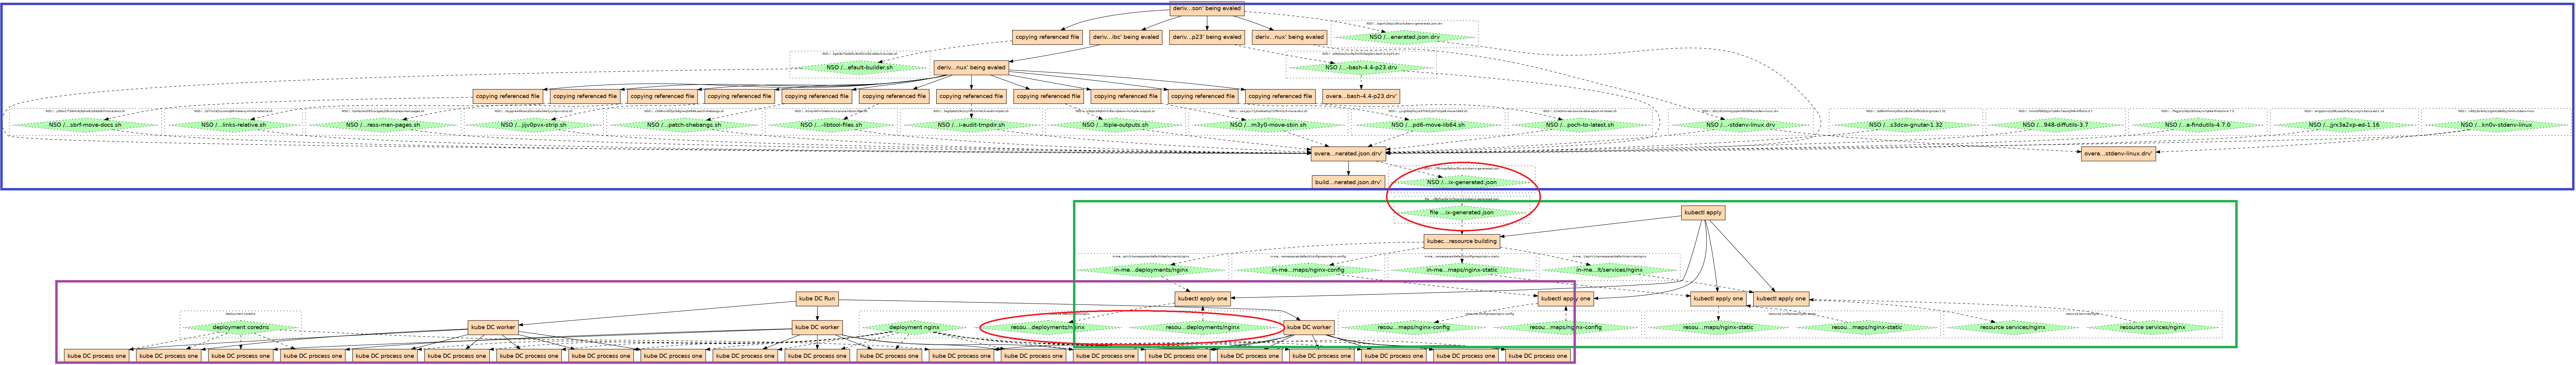
\includegraphics[scale=0.1]{img/huge-graph-3.png}
    \end{sideways}
    \vspace{-1em} 
    \caption{Extract from Tenmo record of a HCPS composed out of Nix / KubeNix, kubectl, and Kubernetes deployment controller.} 
    \label{fig:huge-graph-dot}
\end{figure}

\Cref{fig:huge-graph-dot} represents a Hierarchical Control Plane System composed out of these components and tracked by Tenmo. The top part outlined with indigo color rectangle is an extract from the KubeNix build process for a deployment. The right part outline in light green color is an extract of a record of Kubectl execution (as described in \cref{fig:kubectl}. The bottom part is an extract of a Kubernetes deployments controller performing an intent-based actuation of a deployment resource (as described in \cref{sec:k8s-depl-controller}). Full Tenmo traces would not be possible to visualize in a thesis using existing Graphviz-based tooling.

The Kubnix build and Kubectl execution are related via the file \texttt{kubenix-generated.json} built by Kubenix and consumed by Kubectl. Kubectl and Kuberentes deployments controller are linked via the deployment resource representation submitted to Kubernetes by Kubectl tool. These are marked in red circles in \cref{fig:huge-graph-dot}.

This shows that Tenmo is able to track activity and trace provenance of objects across multiple levels of a hierarchical system. Although this is a simplified example, covers the peculiarities of HCPS systems described in \fullref{sec:intro}.






\begin{comment}

\section{Solution scalability}
%% GP: Czy możemy to w ogóle wywalić? To miało omawiać na ile rozwiązanie się skaluje z kodem, z ludźmi, z systemem, etc?

\subsection{Performance}
%% GP: Czy możemy to pominąć? Wyniki nie będą oszałamiające, a czasu już nie ma.

Rudimentary performance testing has been performed of Nix builds with and without producing JSON logs.

\begin{itemize}
	\item As an extra sanity check, basic performance numbers, not a proper benchmark, maybe show trend with 2x more data.
    \begin{itemize}
    	\item E.g. k8s deployment at size X and 10X, requests still are fast enough
    \end{itemize}
\end{itemize}

TODO: Time to process as events per seconds.


\end{comment}




\begin{comment}
NOTATKI:
\begin{itemize}
\item Uzasadnić dlaczego narzędzie się skaluje lepiej, niż człowiek
\item Skalowanie z linijkami kodu, modułów, zespołów, równolegle wystawianych do produkcji, etc.
\item Wspomnieć o gitops, scaling with repo size, scaling with infrastructure as code, etc.
\end{itemize}
\end{comment}

\newpage
\chapter{Concluding remarks}\label{sec:conclusion}

As shown in~\cref{sec:results}, Tenmo can be applied to a variety of software packages. Tenmo has been shown to be suitable for debugging of build systems, cluster deployment tooling, and cluster orchestration services. We believe that these use cases are representative of a hierarchical control plane system employing intent-based actuation.

\section{System comparison}\label{sec:system-comparison}

Below, we provide a comparison between Tenmo, Dapper~\cite{dapper2010} and ProTracer~\cite{protracer-ma2016}. Dapper and ProTracer are two systems, which we believe are the closest match to our use case. The~\Cref{tbl:comparison} on \cpageref{tbl:comparison} presents a comparison of these systems. As can be seen, they occupy distinct points, in the design space for debuggability solutions.

Section ``HCSP support'' 
%
%MP: odwolanie przez \ref{}
%GP: Tu chodzi o sekcje tabelki, do której odwołuje się 2 słowa dalej. Nie widzę sensu używać \ref tu
%
of~\cref{tbl:comparison} summarizes how these systems compare to the requirements defined in~\cref{sec:reqs}.  We have shown that Tenmo satisfies requirements for a debuggability solution for hierarchical control plane systems employing intent-based actuation.
%%MG: wytłumaczyć co oznacza "--" w tabelce

%%MG: Opisać co to jest kreska w tabeli
\begin{table}[pht]
\centering
\begin{tabular}[t]{  p{5cm}  p{3cm}  p{3cm}  p{3cm}  }
\toprule
&Dapper&ProTracer&Tenmo\\
\midrule
Focus use case&Distributed serving systems&Advanced Persistent Threat&Control plane systems\\
\hline
\multicolumn{4}{c}{Model} \\
\hline
Execution tracing&Yes&Yes&Yes\\
Object tracking&No&Yes&Yes\\
Object versioning&--~$^{1}$&No&Yes\\
Interaction tracking&No~$^{2}$&Yes&Yes\\
\hline
\multicolumn{4}{c}{HCSP support} \\
\hline
Coalescing effects support&--&Yes&Yes\\
Support for abstract entities&--&No&Yes\\
Support for composite entities&--&Yes&Yes\\
Low storage overhead&Yes&No&Yes\\
Full coverage&No&Yes&Yes\\
Gradual fidelity execution tracing&Yes&No&Yes\\
Gradual fidelity provenance tracking&--&Yes&Yes\\
Minimal mental burden&Yes&No&Yes\\
Cross-host tracking&Yes&Yes&Yes\\
Multi-layer systems support&Yes&No&Yes\\
Asynchronous data intake&No&No&Yes\\
Event-based data production&Yes&No&Yes\\
Flexible control flow support&Yes&Yes&Yes\\
\hline
\multicolumn{4}{c}{Application} \\
\hline
Mode&RPC Instrumentation&Auto&Opt-in\\
Trust&Trusted&Untrusted&Trusted\\
\hline
\multicolumn{4}{c}{Other} \\
\hline
Trace sampling&Yes&No&No\\
Maturity&Production&Academic&Academic\\
\bottomrule
\hline
\multicolumn{4}{l}{$^{1}$\footnotesize{Not applicable due to lack of capabilities to track objects.}} \\
\multicolumn{4}{l}{$^{2}$\footnotesize{Dapper does record RPCs, but they are not a first class citizen of the Dapper model.}} \\
\end{tabular}
\caption{Summary system comparison.}
\label{tbl:comparison}
\end{table}%

\section{Model comparison}

Below we discuss how the PEDST model compares to the OpenTracing and to the OpenProvenance models. These comparisons are not meant to be comprehensive, and have introductory nature. However, they provide some birds-eye overview which cna be of value to the reader. Specifically, we show that the Tenmo model is a ``middle-ground'' between the practicality of the OpenTracing, and the high complexity of the OpenProvenance model. Our model is an extension of the OpenTracing model, and can be reduced to a subset of the PROV data model.

\subsection{OpenTracing model}

In the OpenTracing model the main concept is a trace tree, which is a tree of spans, which represent units of work. Edges in the tree indicate a parent-child relationship between spans. An individual ``span is also a log of timestamped records, which encode the span’s start and end time, any RPC timing data, and zero or more application-specific annotations''~\cite[p.3]{dapper2010}.

The main difference of our model is that our model allows not only for the execution tree to be represented, but also allows us to relate execution trees to each other, whenever they interact with each other via read and write operations on entities in the system. Additionally, interactions between executions are modeled more explicitly and independently of the execution of the parent-child relationship. This allows us to recover more than just a trace tree, out of recorded data, but also a causality graph, interaction graph, effects graph and provenance graph (see \fullref{sec:global-graphs} below for definitions).

In implementations of the OpenTracing model, all RPC messages are recorded as payload in annotations, but RPC interactions are not explicitly part of the model. Our model explicitly records messages, since they are often used as a vehicle for propagating information and, hence, are relevant from the perspective of provenance tracking (see~\cref{sec:model-extensions} for details on how messages relate to provenance tracking in PEDST model).

Data for a single OpenTracing span is populated by two processes -- both RPC client and server. In the PEDST model, each side is represented by an \textit{execution}, and their RPC exchange is represented as a single interaction with an appropriate number of messages (usually two for a single synchronous RPC call).

On top of execution tracing, PEDST model enables capturing interactions with objects, in a system, via \textit{operations} and \textit{incarnation}, allowing it to handle coalescing effects and, henceforth, control plane systems with the intent-based actuation.

In this work we have shown that PEDST model is a superset of OpenTracing model, capable of implementing OpenTracing activity tracing and more. Major difference between Tenmo -- as an implementation of the PEDST model -- and all implementations of OpenTracing is lack of sampling, which allows OpenTracing implementations to scale to ultra-large online serving systems at the cost of tracing coverage. Tenmo -- being focused on control plane systems -- is built to provide full coverage of all -- usually mutating -- activities.

% OpenTracing is typically used via tight integration with core libraries, e.g. RPC libraries. Google’s Dapper main strength is ubiquitous availability to all engineers via its deep integration with Google’s infrastructure.

\begin{comment}
BRAK CZASU
\todo{IMAGE: Translation of an example from OpenTracing to Tenmo}
\todo{TABLE: Maybe add translation table}
\end{comment}

\subsection{OpenProvenance}

The OpenProvenance’s PROV data model is a very elaborate model to track provenance, accommodating three different uses of provenance -- agent-centered provenance, object-centered provenance, and process-centered provenance. Our provenance-enhanced distributed systems tracing model has the most similarities with the process-centered provenance. An example of the difference is that our model does not allow to record provenance of an object without capturing a process, which transforms an input object into a given object.

PEDST incarnations can be represented by PROV entities. In PROV, the result of each revision of a thing, in a system, is a new entity. PEDST \textit{entity concept} can be translated to PROV's \textit{specialization concept}. Alternatively PEDST entity concept can  or by marking a group of PROV entities with a description that one was a revision of another. 
%powyzej zdanie -- sprawdzic czy ma sens
The PROV model allows to explicitly track ``wasDerivedFrom'', relationship between its entities, while PEDST model treats this relationship to be implicit, whenever an execution reads one incarnation and writes another. PEDST's sub-incarnations can be represented with PROV’s collections.

PEDST’s executions can be represented by PROV activities. PROV \textit{Start} and \textit{End} can represent beginning and end of an execution. Hierarchical nature of PEDST executions can be represented by meticulous use of PROV ``wasStartedBy''  and ``wasEndedBy''  relationships, between activities. PEDST’s processes can be represented as PROV Plans.

PEDST’s interaction can be represented by PROV Communication concept. PROV has no concept which can represent PEDST messages, but those could be, with some loss of information, be packed into attributes of ``wasInformedBy'' relation.

PEDST’s read and write operations can be represented as PROV Usage and Generation concepts, which ties up the PEDST to PROV translation.

PROV contains many other concepts, like agents, responsibility, influence, delegation, bundles, alternate, collections, etc., which are not representable in the Tenmo model. We have not found these concepts to be particularly useful for our use case~(\cref{sec:use-case}).




%ponizej nie robic

\begin{comment}
BRAK CZASU

\todo{IMAGE: Translation of an example from Tenmo to PROV}
\todo{TABLE: Maybe add translation table}
\end{comment}


\section{Outside of the scope of the work}
%% Podzielić na "Outside of the scope" i na "Future development"

Debuggability of software systems is a vast research area. While working on this thesis we have identified a set of related topics, which we did not pursue as part of this research. We will briefly discuss the relation, why we have not addressed these areas and, in some cases. We'll discuss future development in a next section.

\subsection{Automated provenance gathering}

Although the PEDST model is suitable for use in automated provenance gathering mechanisms, via compiler instrumentation, syscall interception, etc., we believe that automated provenance gathering, if applied to HCPS, will not be successful. Signal-to-noise ratio, in the gathered data, will suffer due to the mismatch between low-level objects, typically suitable for automated provenance gathering, and high-level entities, which HCPS typically operate on. Additionally, it is not obvious how automated provenance gathering will deal with identifying long-living entities and processes, as identifying both is rather subjective, and heavily dependent on the use cases. Moreover, an explosion of data gathered by the system will require additional work to scale the PEDST architecture and the Tenmo framework. 

An alternative research avenue, for automated provenance gathering, is through database instrumentation, which would allow us to track how objects evolve over time, in a system. Kubernetes ecosystem could be suitable for such research, but it is not yet clear how database-based provenance gathering would work in a system using \texttt{etcd} (a NoSQL database). Traditional database provenance research, typically, focuses on relational databases, with built-in query engines, and NoSQL database systems typically do not have these properties.

\subsection{Tamper-resistance}

Tamper-resistance is a non-goal of this work. Control plane systems are typically owned and operated by a single entity, a cloud provider. Hence, there is a reasonable trust for individuals operating the system. These enterprise deployments would, typically, have other mechanisms to ensure safety, privacy and security of any internal systems (e.g. access control, audit logging, etc).

\subsection{Audit logging}

Although there is a large overlap between what audit logging and provenance\hyp{}enhanced distributed tracing are aiming to record, the user experience and requirements towards security of the systems are vastly different. Audit logging research often focuses on security and tamper-resistance of the gathered information.

\subsection{Blockchain provenance}

Blockchain provenance is inherent in the construction of most blockchain systems. Additionally recent blockchain-based systems employing smart contracts have some properties similar to the control plane systems (e.g. interleaving of execution- and object-based interactions). Blockchain systems are inherently based on tracking relationships between blocks -- a property very similar to provenance tracking. This typically happens at a coarse grain of whole blocks. Granular fidelity data provenance tracking could be useful to trace things at smart contract evaluation level, including sub-block data granularity.

\section{Future development}

This work was focused on proving that a proposed model works and is viable for HCPS. The included implementation is a proof-of-concept. Additional work is necessary both to extend the applicability area for PEDST model and to improve its implementation.

\subsection{Implementation scalability}

We exclude the problem of large-scale deployments, be it sampling, ingestion, processing and querying of the data generated by the tracing system. We expect that a Dapper-inspired implementation, to deal with the volume of generated data, to be sufficient. Additional work is going to be necessary to analyze effects of sampling on the provenance tracking aspects of Tenmo. Given a more expressive data model, additional work is necessary to understand  more complex graph-based, and potentially recursive, queries over the data. Additional implementation-specific limitations (e.g. annotation payload size limit) would be necessary for Tenmo framework to scale to large-scale systems.

\subsection{Library-level instrumentation}

The Tenmo model is suitable for the library-level instrumentation, e.g. in RPC libraries, and context propagation libraries, and should be able to follow distributed control paths, with near-zero intervention from application developers. Similarly, as any OpenTracing implementation, distributed tracing can be provided out of the box to application developers, who use Tenmo-instrumented libraries.

We found that there is no single RPC library, which is adopted widely enough in the open-source ecosystems related to HCPS, which would allow us to implement such library-level instrumentation and analyse results.


\subsection{Security}

We believe that the PEDST model, proposed in this thesis, is suitable as a foundation for Advanced Persistent Threat attack detection and investigation solutions (see,~\cite{apt-daly2009}). This could be, one more, direction for future work. The PEDST architecture would have to be adapted to act in a limited trust environment, and will not be able to depend on the white-box instrumentation approach. Clearly, additional work is required to understand implications of switching to a black-box approach.

\section{Contributions}

The main contribution of this thesis is the development of a provenance-enhanced distributed systems tracing model, which we implemented in the Tenmo tracing system. In this model, we combine industry-standard tracing concepts, with provenance tracking mechanisms, as researched in a wide range of provenance research.

We show that the proposed model is a general solution suitable for debugging modern hierarchical control plane systems, which include heterogeneous components acting both in imperative and declarative paradigm, including use of intent-driven actuation. We show that our model is suitable for implementation and practical usage.

In this thesis, we have researched, designed and proven a useful solution in the debuggability landscape. It occupies a unique point in the design space of debugging systems.

This said, main contributions of this thesis can be summarized as follows:
%
\begin{itemize}
	\item Identified distinguishing characteristics of hierarchical control plane systems (HCPS) with intent-based actuation, making the their debuggability an unsolved problem (\cref{sec:problem}).
	\item Applied provenance research results, in a practical software engineering problem of tracing in HCPS.
	\item Identified necessary properties of a debuggability solution, capable of dealing with HCPS (\cref{sec:reqs}).
	\item Defines a provenance-enhanced distributed systems tracing model, extending the OpenTracing distributed systems tracing model with provenance tracking capabilities (\cref{sec:pedst-model}).
	\item To track provenance, in a way compared to the Dapper model, read and write operations performed by each component in a system have been recorded explicitly and treated as first-class citizens of a model (\cref{sec:model-incarnation}).
	% \item To construct a meaningful provenance graph for a HCPS, it is necessary to track revisions of all mutable objects operated on by a system.  [TBD in text, not yet clearly stated]
	\item Presented an architecture, required to perform provenance-enhanced distributed systems tracing for HCPS (\cref{sec:arch}).
	\item Showed an implementation, capable of reconstructing a full provenance and execution graphs, given the logs are gathered according to the logging protocol (\cref{sec:arch}, \cref{sec:impl}).
	% \item Showed necessity to perform logging in a localized manner in relation to each unit of work to allow the tracing model to scale. It is sufficient to perform logging in a localized manner (\cref{sec:logging-model}).
	\item Showed that if the logging is done according to the protocol, a global view on the provenance graph can be recovered (\cref{sec:logging-model}).
	\item Showed that the proposed provenance-enhanced distributed systems tracing model is practical (\cref{sec:results}). 
	% \item Showed correspondence of individual logging protocol requirements with provenance formalisms. [TBD in text]
	\item Showed that provenance-enhanced distributed systems tracing data can be used to infer additional information through over-approximation mechanisms (\cref{sec:model-extensions}).
\end{itemize}

\bigskip

\section{Discussion}

Tenmo has been shown to be able to model, gather and analyse provenance-enhanced tracing data. We have shown that Tenmo is applicable to a number of software systems, and can answer practical debugging questions.

In its current implementation Tenmo tracing is either fully enabled or disabled. There is no mechanism of granular control over tracing. Such control could be implemented and made to work akin to standard logging verbosity runtime settings. This mechanism would allow to trade-off tracing coverage and fidelity versus performance penalty of tracing. Additional work is required to understand impact of such runtime controls over correctness of execution tracing and provenance tracking.

Given that Tenmo is a white-box tracing solution dependent on instrumentation inside of the system under tracing, adoption costs needs to be considered. In our limited experience implementing Tenmo for Nix and Kubernetes, we have found that the process is mostly straightforward and adding logging statements is obvious and cheap. On the other hand we have found that the following hurdles needs to be overcame.
%
\begin{itemize}[nosep]
    \item Propagation of execution identifiers across layers of a single system. Instrumentation of a Go project which pervasively uses Go's Context would also have been easier.
    \item Propagation of a parent execution identifier from the caller to the callee across technologies. A RPC-level instrumentation would simplify integration of Tenmo into a system. W3C Trace Context could be used for HTTP interactions. 
    \item Entity incarnation versioning is not always obvious, can be hard to added to the system under tracing and be of a can be not important for the system itself. For example reading individual files from disk provides no information about their versioning, besides a modification time. Using it as a incarnation version is possible, but requires use of ``inter-incarnation provenance extension'' extension to maintain provenance relationship.
    \item Identifiers coherence across systems. It has been hard to maintain coherent identifiers for executions and incarnations across the systems. This should be doable in a single organization via a policy, but is harder to achieve across organizations and/or in open source world.
\end{itemize}
%
Additional research is necessary to address these issues.

During work on integration of Tenmo in services, we have found that it is useful to manually add human-inferred data for the needs of analysis. For example, a human can infer from the context that two incarnations, produced by two different systems, each with unique identifier, are actually provenance-related. It might be useful to allow a human to ``assert'' such relationships into a ``observed universe'', constructed based on a given dataset. Such assertion, for example, could be structured as an imaginary execution, with read-write operations pair similarly as ``inter-incarnation provenance extension'' (\cref{sec:model-extensions} to make sure that provenance relationship is maintained. This would help developers to manually ``connect the dots'', during interactive development sessions in presence of instrumentation imperfections in the traced system.

Concepts of entities, processes, sub-incarnations and sub-executions allow to aggregate data in various ways. Various data aggregations, in the global model, can be useful to visualize the data to a user in abstracted form, while preserving correctness and improving usefulness. These aggregations should help navigating large provenance and execution graph,s generated in the PEDST model. We expect these to be especially useful for exploratory debugging by software developers, not yet knowledgeable about a system under tracing. Provenance segmentation research~\cite{provenance-segmentation-abreu2016} provides additional avenues for improving signal-to-noise ratio levels of gathered data.

Another aspect of this system, which has not been investigated, and seems to have potential value, is temporal analysis of Tenmo traces. An example is ability to compute a difference between two (or more) historical executions of the same complex process, at different times, in somehow different contexts. This could address a practical problem of ``why did it suddenly stop working today although it was working yesterday?''. Additional research is necessary to formulate this problem in a clear manner, and propose a solution.

Moreover the graph data model, obtained during work on this problem, closely resembles the Resource Description Framework (RDF) triples~\cite{rdf-auer2007dbpedia}. We believe that the existing extensive research on knowledge extraction and data retrieval, in the area of RDF and Semantic Web~\cite{rdf-shadbolt2006semantic}, could be used here to drive further usability of the solution~\cite{rdf-powers2003practical}.

\section{Conclusion}

This research aimed at proposing a debugging solution, applicable to hierarchical control plane system employing intent-based actuation. Based on requirements analysis, use case modelling, sketch of model formalization, and empirical usage prototypes, of the proposed solution in a software stack, representative of hierarchical control plane systems deployed at cloud providers, it can be concluded that the proposed solution is successfully applicable to the focus use case of this work. The results indicate that a large scale debuggability solution, for hierarchical cloud control plane systems, is possible and practical.

Based on these conclusions, practitioners should consider looking into provenance and provenance tracking research to adopt ideas for the next generation of observability solutions.

To better understand the usability of data gathered using the proposed solution, future studies could address problem of efficient knowledge retrieval from the large amounts of data the proposed system would acquire. Further research is needed to determine the best ways to query the data for visualizations in debugging tooling, interactively explore the data, annotate the data manually and, overall, help software engineers use the proposed solution to reason about the distributed systems they own.

Existing debuggability solutions used in industry, and proposed in academia, do not address the specific use case of hierarchical control plane systems. This research addresses this gap, by combining two areas of research: distributed systems tracing and provenance tracking.

\hfill$\blacksquare$

% ------------------------------- BIBLIOGRAPHY ---------------------------

\cleardoublepage % Zaczynamy od nieparzystej strony
\printbibliography[heading=bibintoc]

% \pagenumbering{gobble}
\thispagestyle{empty}


% ----------------------------  LIST OF FIGURES --------------------------------
\clearpage %or \cleardoublepage
\listoffigures
\thispagestyle{empty}

% -----------------------------  LIST OF APPENDICES ---------------------------
\renewcommand{\cftchapaftersnum}{}%
\renewcommand{\cftsecaftersnum}{}% 
\renewcommand{\cftsubsecaftersnum}{}%

% \begin{appendices}
\chapter*{Appendicies}
\addcontentsline{toc}{chapter}{Appendicies}
%\appendix
\section*{Appendix A}
\addcontentsline{toc}{section}{Appendix A}\label{appendix:tenmo-sql-queries-impl}

\textbf{get\_all\_paths\_from} function.

\begin{minted}[fontsize=\scriptsize]{plpgsql}
  CREATE OR REPLACE FUNCTION get_all_paths_from(start text)
  RETURNS TABLE(depth integer, verbs text[], path text[]) AS $$
  BEGIN
  RETURN QUERY

  WITH RECURSIVE search_step(id, link, verb, depth, route, verbs, cycle) AS (
    SELECT r.source, r.target, r.verb, 1,
           ARRAY[r.source],
           ARRAY[r.verb]::text[],
           false
      FROM graph r where r.source=start

     UNION ALL

    SELECT r.source, r.target, r.verb, sp.depth+1,
           sp.route || r.source,
           sp.verbs || r.verb,
           r.source = ANY(route)
      FROM graph r, search_step sp
     WHERE r.source = sp.link AND NOT cycle
  )
  SELECT sp.depth, array_append(sp.verbs, '<end>') AS verbs, sp.route || sp.link AS path
  FROM search_step AS sp
  WHERE NOT cycle
  ORDER BY depth ASC;
\end{minted}

\textbf{get\_all\_paths\_from\_by\_verbs} function.

\begin{minted}[fontsize=\scriptsize]{plpgsql}
  CREATE OR REPLACE FUNCTION get_all_paths_from_by_verbs(start text, crawl_verbs text[])
  RETURNS TABLE(depth integer, verbs text[], path text[]) AS $$
  BEGIN
  RETURN QUERY

  WITH RECURSIVE search_step(id, link, verb, depth, route, verbs, cycle) AS (
    SELECT r.source, r.target, r.verb, 1,
           ARRAY[r.source],
           ARRAY[r.verb]::text[],
           false
      FROM graph r where r.source=start and r.verb = ANY(crawl_verbs)

     UNION ALL

    SELECT r.source, r.target, r.verb, sp.depth+1,
           sp.route || r.source,
           sp.verbs || r.verb,
           r.source = ANY(route)
      FROM graph r, search_step sp
     WHERE r.source = sp.link AND NOT cycle and r.verb = ANY(crawl_verbs)
  )
  SELECT sp.depth, array_append(sp.verbs, '<end>') AS verbs, sp.route || sp.link AS path
  FROM search_step AS sp
  WHERE NOT cycle
  ORDER BY depth ASC;
\end{minted}

\textbf{get\_closure\_from} function.

\begin{minted}[fontsize=\scriptsize]{plpgsql}
  create or replace function get_closure_from(start text)
  returns table(depth integer, obj text) as $$
  begin
  return query
  select t.depth, t.path[array_upper(t.path,1)] from get_all_paths_from(start) as t;
  end;
  $$ language plpgsql;
\end{minted}

\textbf{get\_closure\_from\_filtered} function.

\begin{minted}[fontsize=\scriptsize, breaklines]{plpgsql}
  create or replace function get_closure_from_filtered(start text, filter_verbs text[])
  returns table(depth integer, obj text) as $$
  begin
  return query
  select t.depth, t.path[array_upper(t.path,1)] from get_all_paths_from(start) as t where t.verbs[array_upper(t.verbs,1)-1] = ANY(filter_verbs);
  end;
  $$ language plpgsql;
\end{minted}

\textbf{get\_closure\_from\_by\_verbs} function.

\begin{minted}[fontsize=\scriptsize]{plpgsql}
  CREATE OR REPLACE FUNCTION get_closure_from_by_verbs(start text, crawl_verbs text[])
  RETURNS TABLE(depth integer, obj text) AS $$
  BEGIN
  RETURN QUERY
  select t.depth, t.path[array_upper(t.path,1)] from get_all_paths_from_by_verbs(start, crawl_verbs) as t;
  END;
  $$ LANGUAGE plpgsql;
\end{minted}

\textbf{get\_closure\_from\_by\_verbs\_filtered} function.

\begin{minted}[fontsize=\scriptsize, breaklines]{plpgsql}
  CREATE OR REPLACE FUNCTION get_closure_from_by_verbs_filtered(start text, crawl_verbs text[], filter_verbs text[])
  RETURNS TABLE(depth integer, obj text) AS $$
  BEGIN
  RETURN QUERY
  select t.depth, t.path[array_upper(t.path,1)] from get_all_paths_from_by_verbs(start, crawl_verbs) as t where t.verbs[array_upper(t.verbs,1)-1] = ANY(filter_verbs);
  END;
  $$ LANGUAGE plpgsql;
\end{minted}

\textbf{provenance\_set} function.

\begin{minted}[fontsize=\scriptsize, breaklines]{plpgsql}
 CREATE OR REPLACE FUNCTION provenance_set(start text)
 RETURNS TABLE(depth integer, obj text) AS $$
 BEGIN
 RETURN QUERY
 select * from get_closure_from_by_verbs_filtered(start, ARRAY['written_by','reads']::text[], '{reads}'::text[]) as t where t.depth <= 2;
 END;
 $$ LANGUAGE plpgsql;
\end{minted}

\textbf{provenance\_set\_indirect} function.

\begin{minted}[fontsize=\scriptsize, breaklines]{plpgsql}
 CREATE OR REPLACE FUNCTION provenance_set_indirect(start text)
 RETURNS TABLE(depth integer, obj text) AS $$
 BEGIN
 RETURN QUERY
 select * from get_closure_from_by_verbs_filtered(start, ARRAY['written_by','reads']::text[], '{reads}'::text[]) as t;
 END;
 $$ LANGUAGE plpgsql;
\end{minted}

\textbf{trace} function.

\begin{minted}[fontsize=\scriptsize]{plpgsql}
  CREATE OR REPLACE FUNCTION trace(start text)
  RETURNS TABLE(depth integer, obj text) AS $$
  BEGIN
  RETURN QUERY
  select * from get_closure_from_by_verbs(start, ARRAY['child_of']::text[]) as t;
  END;
  $$ LANGUAGE plpgsql;
\end{minted}
% \end{appendices}
\thispagestyle{empty}


\begin{comment}
==================== COMMENTED OUT BELOW=======================
==================== COMMENTED OUT BELOW=======================
==================== COMMENTED OUT BELOW=======================
==================== COMMENTED OUT BELOW=======================
==================== COMMENTED OUT BELOW=======================

% ----------------------- LIST OF SYMBOLS AND ABBREVIATIONS ------------------
\chapter*{List of Symbols and Abbreviations}
\addcontentsline{toc}{chapter}{List of Symbols and Abbreviations}

\begin{tabular}{cl}
nzw. & nadzwyczajny \\
* & operator gwiazdka \\
$\widetilde{}$ & tylda
\end{tabular}
\\
\thispagestyle{empty}



% -----------------------------  LIST OF TABLES --------------------------------
% \clearpage %or \cleardoublepage
% \listoftables
% \thispagestyle{empty}


\end{comment}

\end{document}
